% LaTeX source for ``Think Stats:
% Probability and Statistics for Programmers''
% Copyright 2011  Allen B. Downey.

% License: Creative Commons Attribution-NonCommercial 3.0 Unported License.
% http://creativecommons.org/licenses/by-nc/3.0/
%

%\documentclass[10pt,b5paper]{book}
\documentclass[12pt]{book}
\usepackage[width=5.5in,height=8.5in,
  hmarginratio=3:2,vmarginratio=1:1]{geometry}
\setlength{\headheight}{15.5pt}

% for some of these packages, you might have to install
% texlive-latex-extra (in Ubuntu)

\usepackage[T1]{fontenc}
\usepackage{textcomp}
\usepackage{mathpazo}

%\usepackage{pslatex}

\usepackage[czech]{babel}
\usepackage[utf8]{inputenc}   % pro unicode UTF-8


\usepackage{url}
\usepackage{fancyhdr}
\usepackage{graphicx}
\usepackage{subfig}
\usepackage{amsmath}
\usepackage{amsthm}
%\usepackage{amssymb}
\usepackage{makeidx}
\usepackage{setspace}
\usepackage{hevea}
\usepackage{upquote}
\usepackage{sectsty}
\usepackage{multicol}

\title{Think Stats}
\author{Allen B. Downey}

\newcommand{\thetitle}{Think Stats: Probability and Statistics for Programmers}
\newcommand{\theversion}{1.6.0}

\usepackage{enumitem}
\setlist[description]{itemindent=0cm,leftmargin=0cm,style=unboxed}

% these styles get translated in CSS for the HTML version
\newstyle{a:link}{color:black;}
\newstyle{p+p}{margin-top:1em;margin-bottom:1em}
\newstyle{img}{border:0px}

% change the arrows in the HTML version
\setlinkstext
  {\imgsrc[ALT="Previous"]{back.png}}
  {\imgsrc[ALT="Up"]{up.png}}
  {\imgsrc[ALT="Next"]{next.png}}

\makeindex

\newif\ifplastex
\plastexfalse

\begin{document}

\frontmatter

\ifplastex
    \newcommand{\dd}{\mathit{d}}
    \newcommand{\e}{\mathit{e}}
    \newcommand{\f}{\mathit{f}}
    \newcommand{\gee}{\mathit{g}}
    \newcommand{\ii}{\mathit{i}}
    \newcommand{\kk}{\mathit{k}}
    \newcommand{\n}{\mathit{n}}
    \newcommand{\m}{\mathit{m}}
    \newcommand{\w}{\mathit{w}}
    \newcommand{\p}{\mathit{p}}
    \newcommand{\s}{\mathit{s}}
    \newcommand{\x}{\mathit{x}}
    \newcommand{\X}{\mathit{X}}
    \newcommand{\y}{\mathit{y}}
    \newcommand{\Y}{\mathit{Y}}
    \newcommand{\z}{\mathit{z}}
    \newcommand{\Z}{\mathit{Z}}
    \newcommand{\E}{\mathit{E}}
    \newcommand{\OO}{\mathit{O}}
    \newcommand{\HH}{\mathit{H}}
    \newcommand{\A}{\mathit{A}}
    \newcommand{\B}{\mathit{B}}
    \newcommand{\D}{\mathit{D}}
    \newcommand{\N}{\mathit{N}}
    \newcommand{\R}{\mathit{R}}
    \newcommand{\Ssq}{$S^2$}
    \newcommand{\Snsq}{$S_{n-1}^2$}
    \newcommand{\mya}{\mathit{a}}
    \newcommand{\myb}{\mathit{b}}
    \newcommand{\Prob}{\mathit{P}}
    \newcommand{\xsubi}{\mathit{x}\sub{i}}
    \newcommand{\psubi}{\mathit{p}\sub{i}}
    \newcommand{\mymu}{\mathit{\mu}}
    \newcommand{\mychi}{\mathit{\chi}}
    \newcommand{\myalpha}{\mathit{\alpha}}
    \newcommand{\mysigma}{\mathit{\sigma}}
    \newcommand{\myrho}{\mathit{\rho}}
    \newcommand{\mylambda}{\mathit{\lambda}}
    \newcommand{\mydelta}{\mathit{\delta}}
    \newcommand{\sigmasq}{\mathit{\sigma}\super{2}}

    \newcommand{\plus}{+}
    \newcommand{\mytimes}{\times}
    \newcommand{\mydivide}{/}
    \newcommand{\mystar}{\lowast}
    \newcommand{\mysim}{\sim}
    \newcommand{\myapprox}{\approx}
    \newcommand{\mynormal}{$\mathcal{N}$}

    \newcommand{\myslope}{\mathit{\beta}}
    \newcommand{\myinter}{\mathit{\alpha}}

    \newcommand{\myeps}{\mathit{\varepsilon}}
    \newcommand{\myxbar}{\uxbar}
    \newcommand{\myybar}{\uybar}
    \newcommand{\mynhat}{$\nhat$}
    \newcommand{\myle}{\ule}
\else
    \newcommand{\dd}{$d$}
    \newcommand{\e}{$e$}
    \newcommand{\f}{$f$}
    \newcommand{\gee}{$g$}
    \newcommand{\ii}{$i$}
    \newcommand{\kk}{$k$}
    \newcommand{\n}{$n$}
    \newcommand{\m}{$m$}
    % \newcommand{\w}{$w$}
    \newcommand{\p}{$p$}
    \newcommand{\s}{$s$}
    \newcommand{\x}{$x$}
    \newcommand{\X}{$X$}
    \newcommand{\y}{$y$}
    \newcommand{\Y}{$Y$}
    \newcommand{\z}{$z$}
    \newcommand{\Z}{$Z$}
    \newcommand{\E}{$E$}
    \newcommand{\OO}{$O$}
    \newcommand{\HH}{$H$}
    \newcommand{\A}{$A$}
    \newcommand{\B}{$B$}
    \newcommand{\D}{$D$}
    \newcommand{\N}{$N$}
    \newcommand{\R}{$R$}
    \newcommand{\Ssq}{$S^2$}
    \newcommand{\Snsq}{$S_{n-1}^2$}
    \newcommand{\mya}{$a$}
    \newcommand{\myb}{$b$}
    \newcommand{\Prob}{$P$}
    \newcommand{\xsubi}{$x_i$}
    \newcommand{\psubi}{$p_i$}
    \newcommand{\mymu}{$\mu$}
    \newcommand{\mychi}{$\chi$}
    \newcommand{\myalpha}{$\alpha$}
    \newcommand{\mysigma}{$\sigma$}
    \newcommand{\myrho}{$\rho$}
    \newcommand{\mylambda}{$\lambda$}
    \newcommand{\mydelta}{$\delta$}
    \newcommand{\sigmasq}{$\sigma^2$}

    \newcommand{\plus}{$+$}
    \renewcommand{\minus}{$-$}
    \newcommand{\mytimes}{$\times$}
    \newcommand{\mydivide}{$/$}

    \newcommand{\sub}[1]{$_{#1}$}
    \newcommand{\super}[1]{$^{#1}$}
    \newcommand{\mystar}{$\star$}
    \newcommand{\mysim}{$\sim$}
    \newcommand{\myapprox}{$\approx$}
    \newcommand{\normal}{\mathcal{N}}
    \newcommand{\mynormal}{$\mathcal{N}$}

    \newcommand{\myslope}{$\beta$}
    \newcommand{\myinter}{$\alpha$}

    \newcommand{\myeps}{$\varepsilon$}

    \newcommand{\myxbar}{$\xbar$}
    \newcommand{\myybar}{$\ybar$}
    \newcommand{\mynhat}{$\nhat$}
    \newcommand{\myle}{$\le$}
    \newcommand{\Eqn}[1]{\quad #1}
\fi

\newcommand{\Erdos}{Erd\H{o}s}
\newcommand{\nhat}{\hat{N}}
\newcommand{\eps}{\varepsilon}
\newcommand{\slope}{\beta}
\newcommand{\inter}{\alpha}
\newcommand{\xbar}{\bar{x}}
\newcommand{\ybar}{\bar{y}}
\newcommand{\PMF}{\mathrm{PMF}}
\newcommand{\PDF}{\mathrm{PDF}}
\newcommand{\CDF}{\mathrm{CDF}}
\newcommand{\ICDF}{\mathrm{ICDF}}

\ifplastex
    \usepackage{localdef}
    \maketitle

\newcount\anchorcnt
\newcommand*{\Anchor}[1]{%
  \@bsphack%
    \Hy@GlobalStepCount\anchorcnt%
    \edef\@currentHref{anchor.\the\anchorcnt}%
    \Hy@raisedlink{\hyper@anchorstart{\@currentHref}\hyper@anchorend}%
    \M@gettitle{}\label{#1}%
    \@esphack%
}


\else

%%% EXERCISE

\newtheoremstyle{exercise}% name of the style to be used
  {\topsep}% measure of space to leave above the theorem. E.g.: 3pt
  {\topsep}% measure of space to leave below the theorem. E.g.: 3pt
  {}% name of font to use in the body of the theorem
  {0pt}% measure of space to indent
  {\bfseries}% name of head font
  {}% punctuation between head and body
  { }% space after theorem head; " " = normal interword space
  {}% Manually specify head

\theoremstyle{exercise}
\newtheorem{exercise}{Cvičení}[chapter]

%\newcounter{exercise}[chapter]
%\newcommand{\nextexercise}{\refstepcounter{exercise}}

%\newenvironment{exercise}{\nextexercise \noindent \textbf{Cvičení \thechapter.\theexercise} \begin{itshape} \noindent}{\end{itshape}}

\sloppy
%\setlength{\topmargin}{-0.375in}
%\setlength{\oddsidemargin}{0.0in}
%\setlength{\evensidemargin}{0.0in}

% Uncomment these to center on 8.5 x 11
%\setlength{\topmargin}{0.625in}
%\setlength{\oddsidemargin}{0.875in}
%\setlength{\evensidemargin}{0.875in}

%\setlength{\textheight}{7.2in}

\setlength{\headsep}{3ex}
\setlength{\parindent}{0.0in}
\setlength{\parskip}{1.7ex plus 0.5ex minus 0.5ex}
\renewcommand{\baselinestretch}{1.02}

% see LaTeX Companion page 62
\setlength{\topsep}{-0.0\parskip}
\setlength{\partopsep}{-0.5\parskip}
\setlength{\itemindent}{0.0in}
\setlength{\listparindent}{0.0in}

% see LaTeX Companion page 26
% these are copied from /usr/local/teTeX/share/texmf/tex/latex/base/book.cls
% all I changed is afterskip

\makeatletter

\renewcommand{\section}{\@startsection 
    {section} {1} {0mm}%
    {-3.5ex \@plus -1ex \@minus -.2ex}%
    {0.7ex \@plus.2ex}%
    {\normalfont\Large\bfseries}}
\renewcommand\subsection{\@startsection {subsection}{2}{0mm}%
    {-3.25ex\@plus -1ex \@minus -.2ex}%
    {0.3ex \@plus .2ex}%
    {\normalfont\large\bfseries}}
\renewcommand\subsubsection{\@startsection {subsubsection}{3}{0mm}%
    {-3.25ex\@plus -1ex \@minus -.2ex}%
    {0.3ex \@plus .2ex}%
    {\normalfont\normalsize\bfseries}}

% The following line adds a little extra space to the column
% in which the Section numbers appear in the table of contents
\renewcommand{\l@section}{\@dottedtocline{1}{1.5em}{3.0em}}
\setcounter{tocdepth}{1}

\makeatother

\newcommand{\beforefig}{\vspace{1.3\parskip}}
\newcommand{\afterfig}{\vspace{-0.2\parskip}}

\newcommand{\beforeverb}{\vspace{0.6\parskip}}
\newcommand{\afterverb}{\vspace{0.6\parskip}}

\newcommand{\adjustpage}[1]{\enlargethispage{#1\baselineskip}}


% Note: the following command seems to cause problems for Acroreader
% on Windows, so for now I am overriding it.
%\newcommand{\clearemptydoublepage}{
%            \newpage{\pagestyle{empty}\cleardoublepage}}
\newcommand{\clearemptydoublepage}{\cleardoublepage}

%\newcommand{\blankpage}{\pagestyle{empty}\vspace*{1in}\newpage}
\newcommand{\blankpage}{\vspace*{1in}\newpage}

% HEADERS

\renewcommand{\chaptermark}[1]{\markboth{#1}{}}
\renewcommand{\sectionmark}[1]{\markright{\thesection\ #1}{}}

\lhead[\fancyplain{}{\bfseries\thepage}]%
      {\fancyplain{}{\bfseries\rightmark}}
\rhead[\fancyplain{}{\bfseries\leftmark}]%
      {\fancyplain{}{\bfseries\thepage}}
\cfoot{}

\pagestyle{fancyplain}


% turn off the rule under the header
%\setlength{\headrulewidth}{0pt}

% the following is a brute-force way to prevent the headers
% from getting transformed into all-caps
\renewcommand\MakeUppercase{}

% Exercise environment
\newtheoremstyle{myex}% name
     {9pt}%      Space above
     {9pt}%      Space below
     {}%         Body font
     {}%         Indent amount (empty = no indent, \parindent = para indent)
     {\bfseries}% Thm head font
     {}%        Punctuation after thm head
     {0.5em}%     Space after thm head: " " = normal interword space;
           %       \newline = linebreak
     {}%         Thm head spec (can be left empty, meaning `normal')

\theoremstyle{myex}


\begin{latexonly}

\renewcommand{\blankpage}{\thispagestyle{empty} \quad \newpage}

%\blankpage
%\blankpage

% TITLE PAGES FOR LATEX VERSION

%-half title--------------------------------------------------
\thispagestyle{empty}

\begin{flushright}
\vspace*{2.0in}

\begin{spacing}{3}
{\huge Think Stats: Pravděpodobnost a statistika pro programátory}\\
{\Large }
\end{spacing}

\vspace{0.25in}

Verze \theversion

\vfill

\end{flushright}

%--verso------------------------------------------------------

\blankpage
\blankpage
%\clearemptydoublepage
%\pagebreak
%\thispagestyle{empty}
%\vspace*{6in}

%--title page--------------------------------------------------
\pagebreak
\thispagestyle{empty}

\begin{flushright}
\vspace*{2.0in}

\begin{spacing}{3}
{\huge Think Stats}\\
{\Large Pravděpodobnost a statistika pro programátory}
\end{spacing}

\vspace{0.25in}

{\Large
Allen B. Downey\\
}



\vspace{1.5in}

Flow \\
Brno, 2014 \\
ISBN XXXXXX \\
Přeloženo z verze \theversion

%\includegraphics[width=1in]{figs/logo1.eps}
\vfill

\end{flushright}


%--copyright--------------------------------------------------
\pagebreak
\thispagestyle{empty}

{\small
Copyright \copyright ~2011 Allen B. Downey. \\
Překlad \copyright ~2014 Jaroslava Žgáničová. \\
Obálka \copyright ~2014 Matěj Málek.

\vspace{0.2in}

\begin{flushleft}
V roce 2014 vydalo nakladatelství Flow, o.s. \\
IČ: 01549316 \\
Adresa: Brno--Líšeň, \\
Hochmanova 2177/13 \\
\end{flushleft}

ISBN XXXXXX

Tento dokument je možné kopírovat, šířit a/nebo upravovat v souladu s podmínkami licence Creative Commons Attribution-NonCommercial 3.0 Unported, jejíž znění je dostupné na \url{http://creativecommons.org/licenses/by-nc/3.0/}.

Originální formou této knihy je zdrojový kód \LaTeX. Kompilací tohoto kódu vzniká zobrazení učebnice, které je nezávislé na konkrétním zařízení a může být převedeno do jiných formátů a vytištěno.

Zdrojový kód \LaTeX\ českého překladu této knihu je dostupný na \url{https://github.com/ThinkStatsCs/ThinkStatsCs}. Zdrojový kód původního textu knihy je dostupný na
\url{http://thinkstats.com}.


\vspace{0.2in}

} % end small

\end{latexonly}


% HTMLONLY

\begin{htmlonly}

% TITLE PAGE FOR HTML VERSION

{\Large \thetitle}

{\large Allen B. Downey}

Version \theversion

\vspace{0.25in}

Copyright 2011 Allen B. Downey

\vspace{0.25in}

Permission is granted to copy, distribute, and/or modify this document
under the terms of the Creative Commons Attribution-NonCommercial 3.0
Unported License, which is available at
\url{http://creativecommons.org/licenses/by-nc/3.0/}.

\setcounter{chapter}{-1}

\end{htmlonly}

\fi
% END OF THE PART WE SKIP FOR PLASTEX

\chapter{Předmluva}
\label{preface}

\section*{Proč jsem napsal tuto knihu}

{\em Think Stats: Pravděpodobnost a statistika pro programátory} je učebnice pro nový typ kurzu poskytující úvod do pravděpodobnosti a statistiky. Důraz je kladen na využití statistických metod při práci s velkými soubory dat. Východiskem je výpočetní přístup, který má hned několik předností:


\begin{itemize}

\item Psaní programů slouží studentům jako nástroj, jak rozvíjet a testovat porozumění probírané látce. Píší například funkce pro výpočet metody nejmenších čtverců, reziduí a determinačního koeficientu. Psaní a testování tohoto kódu se neobejde bez porozumění příslušným konceptům a implicitně také koriguje případné nepochopení.

\item Studenti provádějí experimenty, jejichž cílem je otestovat statistické chování. Například prozkoumávají centrální limitní větu tím, že generují vzorky z různých rozdělení. Ve chvíli, kdy vidí, že součet hodnot z Paretova rozdělení nekonverguje k normálnímu rozdělení, si uvědomí předpoklady, na nichž je centrální limitní věta založena.

\item Některé myšlenky, které je obtížné uchopit matematicky, je snadné pochopit na základě simulace. Provádíme například aproximaci p-hodnot pomocí simulací Monte Carlo, čímž narůstá význam p-hodnoty.

\item Díky použití spojitých rozdělení a výpočtů je možné představit také témata jako například bayesovský odhad, která nejsou běžně součástí úvodních kurzů. V jednom cvičení jsou studenti například požádáni, aby vypočítali aposteriorní rozdělení pro ``problém německého tanku'', což je složité v rámci analytického přístupu, ale překvapivě jednoduché, použijeme-li výpočetní přístup.

\item Vzhledem k tomu, že studenti pracují v univerzálním programovacím jazyku (Python), jsou schopni importovat data téměř z jakéhokoliv zdroje. Nemusí se omezit pouze na data, která byla očištěna a naformátována pro konkrétní statistický nástroj.

\end{itemize}

Kniha je vhodná pro projektový přístup. V mém kurzu pracují studenti na semestrálním projektu, v rámci kterého si mají položit statistickou otázku, najít soubor dat, který jim na ni může dát odpověď, a aplikovat každou z probíraných technik na jejich vlastní data.

Jako ukázka typu analýzy, jaký od svých studentů očekávám, slouží případová studie, která se prolíná celou knihou.  Tato případová studie využívá data ze dvou zdrojů:

\begin{itemize}

\item Národní šetření růstu rodin (National Survey of Family Growth -- NSFG), prováděné Americkými centry pro kontrolu a prevenci nemocí (U. S. Centers for Disease Control and Prevention -- CDC), jehož cílem je shromáždit
  ``informace o rodinném životě, sňatcích a rozvodech, těhotenstvích, neplodnosti, užívání antikoncepce a zdraví mužů a žen''.
  (Viz \url{http://cdc.gov/nchs/nsfg.htm}.)

\item Systém sledování rizikových faktorů chování (Behavioral Risk Factor Surveillance System -- BRFSS),
  prováděný Národním centrem pro prevenci chronických onemocnění a podporu zdraví (National Center for Chronic Disease Prevention and Health Promotion) za účelem ``sledování zdravotních podmínek a rizikového chování ve Spojených státech''.  (Viz \url{http://cdc.gov/BRFSS/}.)

\end{itemize}

V ostatních příkladech jsou využívána data zpřístupněná Daňovou správou USA (IRS), Americkým úřadem pro sčítání lidu a Bostonským maratonem.


\section*{Jak jsem napsal tuto knihu}

Když někdo píše novou učebnici, obvykle začne tím, že přečte stohy starých učebnic. Ve výsledku pak většina učebnic obsahuje stejný materiál v prakticky stejném pořadí. Často se vyskytují fráze a chyby, které se šíří od jedné knihy k další. Stephen Jay Gould upozornil na jeden příklad ve své eseji: ``The Case of
the Creeping Fox Terrier (Případ plíživého foxteriéra)\footnote{Psí plemeno zhruba poloviční velikosti Hyracotheria (viz
  \url{http://wikipedia.org/wiki/Hyracotherium}).}.''

Já jsem takto nepostupoval. Vlastně jsem v průběhu psaní této knihy nepoužil téměř žádné tištěné materiály, a to z několika důvodů:

\begin{itemize}

\item Mým cílem bylo prozkoumat nový přístup k tomuto materiálu, a tak jsem nechtěl být příliš vystaven existujícím přístupům.

\item Protože tuto knihu zpřístupňuji pod volnou licencí, chtěl jsem si být jistý tím, že žádná její část nebude zatížena autorskoprávními omezeními.

\item Mnozí čtenáři mých knih nemají přístup ke knihovnám s tištěnými materiály, a tak jsem se snažil odkazovat na zdroje, které jsou volně dostupné na internetu.

\item Zastánci starých médií si myslí, že výlučné využívání elektronických zdrojů je znakem lenosti a nespolehlivosti. Možná mají pravdu, pokud jde o to první, ale myslím si, že se mýlí v tom druhém bodě, a tak jsem chtěl otestovat svoji teorii.

% http://www.ala.org/ala/mgrps/rts/nmrt/news/footnotes/may2010/in_defense_of_wikipedia_bonnett.cfm

\end{itemize}

Zdroj, který jsem využíval víc než kterýkoliv jiný, je Wikipedie, postrach knihovníků všude na světě. Obecně mohu říci, že články, které jsem si přečetl o statistických tématech, byly velmi dobré (i když jsem v průběhu psaní provedl několik drobných změn). Odkazy na stránky na Wikipedii uvádím na mnoha místech své knihy a doporučuji vám se na tyto odkazy podívat. V řadě případů uvedená stránka na Wikipedii pokračuje tam, kde jsem se svým výkladem skončil. Termíny a způsob zápisu používané v této knize jsou obecně konzistentní s Wikipedií, až na případy, kdy jsem měl dobrý důvod pro odchýlení se.

Další užitečné zdroje, na které jsem narazil, jsou Wolfram MathWorld a (samozřejmě)
Google. Také jsem použil dvě knihy, dílo Davida MacKaye {\em Information
  Theory, Inference, and Learning Algorithms}, což je kniha, která mě přivedla k bayesovské statistice, a dále dílo Press et al. {\em
  Numerical Recipes in C}. Obě knihy jsou ale dostupné také online,
a tak jsem bez obav.

Allen B. Downey \\*
Needham MA \\*

Allen B. Downey je profesorem počítačové vědy na Franklin W. Olin College of Engineering.




%\section*{Acknowledgements}



\section*{Seznam přispěvatelů}

Máte-li nějakou připomínku nebo návrh na opravu, kontaktujte mě prosím prostřednictvím e-mailu
{\tt downey@allendowney.com}. Jestliže na základě vaší zpětné vazby provedu nějakou změnu, přidám vaše jméno na seznam přispěvatelů (pokud mě nepožádáte, abych vaše jméno neuváděl).
\index{přispěvatelé}

Když ve zprávě uvedete alespoň část věty, ve které se chyba objevuje, usnadníte mi tím hledání. Číslo strany a oddílu jsou také dobré, ale nepracuje se s nimi tak snadno.
Díky!

\small

\begin{itemize}

\item Lisa Downey a June Downey si přečetly počáteční verzi a provedly řadu oprav a poskytly mi spoustu připomínek.

\item Steven Zhang objevil několik chyb.

\item Andy Pethan a Molly Farison mi pomohli odladit některá řešení a Molly si všimla několika překlepů.

\item Andrew Heine našel chybu v mé chybové funkci.

\item Dr. Nikolas Akerblom ví, jak velké je Hyracotherium.

\item Alex Morrow vyjasnil jeden z příkladů kódu.

\item Jonathan Street zachytil chybu právě včas.

\item G\'{a}bor Lipt\'{a}k našel překlep v knize a řešení štafetového zápasu.

\item Velké díky patří Kevinu Smithovi a Timu Arnoldovi za jejich práci na plasTeXu, který jsem použil ke konverzi této knihy na DocBook.

\item George Caplan mi poslal několik návrhů pro lepší srozumitelnost.

\item Julian Ceipek našel chybu a několik překlepů.

\item Stijn Debrouwere, Leo Marihart III, Jonathan Hammler a Kent Johnson
našli chyby v prvním tištěném vydání.

\item Dan Kearney našel překlep.

\item Jeff Pickhardt našel nefunkční odkaz a překlep.

\item J\"{o}rg Beyer našel v knize překlepy a provedl řadu oprav v dokumentačních řetězcích (docstrings) doprovodného kódu.

\item Tommie Gannert poslal opravný soubor s řadou oprav.

\item Alexander Gryzlov navrhl objasnění v jednom cvičení.

\item Martin Veillette mi nahlásil chybu v jednom ze vzorců pro Pearsonovu korelaci.

\item Christoph Lendenmann mě upozornil na několik tiskových chyb.

% ENDCONTRIB

\end{itemize}

\normalsize

\clearemptydoublepage

% TABLE OF CONTENTS
\begin{latexonly}

\tableofcontents

\clearemptydoublepage

\end{latexonly}

% START THE BOOK
\mainmatter


\chapter{Statistické myšlení pro programátory}
\label{intro}

Tato kniha se zabývá tím, jak přetavit data ve znalosti.  Data jsou levná (tedy alespoň relativně). Znalosti se získávají obtížněji.

Představím zde tři oblasti, které spolu souvisejí:

\begin{description}

\item[Pravděpodobnost] zkoumá náhodné jevy.  Většina lidí intuitivně rozumí tomu, co jsou stupně
  pravděpodobnosti, a proto můžeme používat slova jako "pravděpodobně" a "nepravděpodobný", aniž bychom prošli speciální přípravou. My však budeme mluvit o tom, jak tyto stupně kvantitativně vyjádřit.
\index{pravděpodobnost}

\item[Statistika] je obor, který na základě vzorků dat vyvozuje určitá tvrzení o populacích.  Většina statistických analýz vychází z pravděpodobnosti, a tak jsou tyto dvě oblasti obvykle prezentovány společně.
\index{statistika}

\item[Výpočty] jsou vhodným nástrojem pro kvantitativní analýzu, ke zpracování statistických údajů se přitom často využívají počítače. Výpočetní experimenty jsou také užitečné při zkoumání konceptů v oblasti pravděpodobnosti a statistiky.
\index{výpočty}

\end{description}

Tato kniha vychází z teze, že pokud umíte programovat, můžete této dovednosti využít k pochopení pravděpodobnosti a statistiky. Tato témata jsou často prezentována z pohledu matematiky a tento postup některým lidem vyhovuje. S některými důležitými myšlenkami v této oblasti je obtížné pracovat matematicky, ale je poměrně snadné uchopit je výpočetně.

Zbytek této kapitoly je věnován případové studii motivované otázkou, kterou jsem zaslechl, když jsme s mojí ženou čekali naše první dítě, a sice: Rodí se prvorozené děti se zpožděním?
\index{prvorozené děti}

\section{\protect\raggedright Rodí se prvorozené děti se zpožděním?}

Když zadáte tento dotaz do Googlu, najdete spoustu diskusí na toto téma. Někteří lidé tvrdí, že je to pravda, jiní zase, že je to mýtus, a někteří tvrdí, že je to naopak: že se prvorozené děti rodí předčasně.

V těchto diskusích se také lidé snaží podepřít svoje tvrzení daty. Našel jsem spoustu takovýchto příkladů:

\begin{quote}

``Dvě mé kamarádky, které nedávno porodily své první dítě, OBĚ téměř 2 týdny přenášely, než u nich začaly porodní bolesti nebo jim je doktoři vyvolali.''

``Moje první dítě se narodilo o 2 týdny později. Teď to ale vypadá, že se druhé narodí o dva týdny před termínem!!''

``Nemyslím si, že by to mohla být pravda, protože moje sestra, která je prvorozená, se mé matce narodila předčasně a stejně tomu bylo i u mnoha mých bratranců a sestřenic. ''

\end{quote}

Takovéto zprávy se označují jako {\bf anekdotické důkazy}, protože se zakládají na údajích, které jsou nepublikované a obvykle mají osobní charakter.  Na takovýchto historkách není nic špatného, pokud se objevují v běžné konverzaci, a tak se nechci do lidí, které jsem tady citoval, nijak navážet.
\index{anekdotický důkaz}

My bychom ale mohli chtít přesvědčivější důkazy a spolehlivější odpovědi. Tomuto standardu anekdotické důkazy většinou nedostojí, a to z následujících důvodů:

\begin{description}

\item[Malý počet pozorování:] Jestliže těhotenství trvá v případě prvorozených dětí déle, rozdíl bude pravděpodobně malý v porovnání s přirozenou variabilitou. V takovém případě bychom zřejmě museli porovnat velký počet těhotenství, abychom si mohli být jisti, že takový rozdíl opravdu existuje.
\index{rozsah vzorku}

\item[Selektivní zkreslení:] Lidé, kteří se zapojují do diskuse o této otázce, by mohli být zainteresovaní, protože jejich první dítě se narodilo se zpožděním. V takovém případě by výsledky byly zkresleny procesem výběru dat.
\index{selektivní zkreslení}
\index{zkreslení!selektivní}

\item[Konfirmační zkreslení:] U lidí, kteří tomuto tvrzení věří, bychom mohli očekávat větší pravděpodobnost, že přispějí nějakými potvrzujícími příklady. U lidí, kteří o tomto tvrzení pochybují, zase existuje větší pravděpodobnost, že budou uvádět protichůdné příklady.
\index{konfirmační zkreslení}
\index{zkreslení!konfirmační}

\item[Nepřesnost:] Historky jsou často osobní příběhy a jako takové si je lidé často nepřesně pamatují, nepřesně vyprávějí a opakují atd.

\end{description}

Takže jak bychom na to mohli jít lépe?

\section{\protect\raggedright Statistický přístup}

Jako způsob, jak se vypořádat s omezeními historek, použijeme statistické nástroje, mimo jiné:

\begin{description}

\item[Sběr dat:] Použijeme data z velkého národního šetření, které bylo navrženo speciálně s cílem dospět ke statisticky validním závěrům ohledně americké populace.
\index{sběr dat}

\item[Popisná statistika:] Vygenerujeme statistické charakteristiky, které výstižně shrnou data, a vyhodnotíme různé způsoby vizualizace dat.
\index{popisná statistika}

\item[Explorační analýza dat:] Budeme hledat vzory, rozdíly a další znaky, které nám pomohou najít odpovědi na otázky, jež nás zajímají. Zároveň se budeme mít na pozoru před nekonzistentností a budeme si uvědomovat omezení.
\index{explorační analýza dat}

\item[Testování hypotéz:] V případě pozorovaných zjištění, jako například rozdílu mezi dvěma skupinami, vyhodnotíme, zda je takové zjištění skutečné, nebo jestli k němu mohlo dojít náhodně.
\index{testování hypotéz}

\item[Odhad:] Použijeme data z výběrového souboru k odhadu vlastností obecné populace.
\index{odhad}

\end{description}

Provedeme-li tyto kroky pečlivě, tak abychom se vyhnuli různým úskalím, můžeme dospět k závěrům, které jsou mnohem lépe podložené a u kterých existuje větší pravděpodobnost, že jsou správné.


\section{\protect\raggedright Národní šetření růstu rodin}
\label{nsfg}

Od roku 1973 provádějí Americká centra pro kontrolu a prevenci nemocí (U.S. Centers for Disease Control and Prevention -- CDC) Národní šetření růstu rodin (National Survey of Family Growth -- NSFG), jehož cílem je shromáždit ``informace o rodinném životě, sňatcích a rozvodech, těhotenstvích, neplodnosti, užívání antikoncepce a zdraví mužů a žen. Výsledky tohoto šetření se využívají... k plánování zdravotnických služeb a programů zdravotního vzdělávání a také k provádění statistických studií rodin, plodnosti a zdraví.''\footnote{Viz
  \url{http://cdc.gov/nchs/nsfg.htm}.}
\index{Národní šetření růstu rodin -- National Survey of Family Growth}
\index{NSFG}

Data shromážděná v rámci tohoto šetření použijeme k prozkoumání otázky, zda se prvorozené děti opravdu rodí se zpožděním, a dalších otázek. Abychom byli schopni používat tato data efektivně, je nezbytné rozumět designu uvedené studie.

Šetření NSFG představuje {\bf průřezovou} studii, což znamená, že zachycuje stav určité skupiny v konkrétním okamžiku. Nejběžnější alternativou je {\bf longitudinální} studie, která se věnuje pozorování jisté skupiny opakovaně po určitou dobu.
\index{průřezová studie}
\index{studie!průřezová}
\index{longitudinální studie}
\index{studie!longitudinální}

Šetření NSFG bylo provedeno sedmkrát; jednotlivé realizace tohoto šetření se nazývají {\bf cykly}.  My budeme používat data z Cyklu 6, který probíhal od ledna 2002 do března 2003.
\index{cyklus}

Cílem tohoto šetření je vyvodit závěry ohledně konkrétní {\bf populace}; v případě šetření NSFG jsou cílovou populací lidé žijící ve Spojených státech ve věku 15--44 let.
\index{populace}

Lidé účastnící se šetření se nazývají {\bf respondenti};
skupina respondentů, která má společný charakteristický znak (věk, pohlaví, vzdělání atp.), se označuje jako {\bf kohorta}.
Obecně se dá říci, že průřezové studie by měly být {\bf
 reprezentativní}, což znamená, že každý člen cílové populace má stejnou šanci se zúčastnit. Tento ideál je pochopitelně v praxi obtížně realizovatelný, ale lidé provádějící šetření se mu snaží maximálně přiblížit.
\index{respondent}
\index{reprezentativní}

Šetření NSFG není reprezentativní. Určité skupiny jsou v něm záměrně nadreprezentovány ({\bf
oversampled}).  Při přípravě studie byly tři skupiny -- Hispánci, Afroameričané a teenageři -- zastoupeny více, než jaké je jejich zastoupení v populaci USA.
Důvodem pro takovéto nadreprezentování (oversampling) bylo zajistit, aby počet respondentů z každé z těchto skupin byl dostatečně velký pro vyvození validních statistických závěrů.
\index{nadreprezentování}

Nevýhodou nadreprezentování pochopitelně je, že na základě statistických údajů zjištěných v rámci šetření již není tak snadné činit závěry o obecné populaci. K tomuto se ještě vrátíme později.

\begin{exercise}

Přestože bylo šetření NSFG provedeno sedmkrát, nejedná se o longitudinální studii. Na toto téma si přečtěte stránky na Wikipedii
\url{http://wikipedia.org/wiki/Cross-sectional_study}
a
\url{http://wikipedia.org/wiki/Longitudinal_study}, abyste se ujistili, že rozumíte, proč tomu tak je.

\end{exercise}

\begin{exercise}

V tomto cvičení si stáhnete data z NSFG. Tato data budeme využívat v celé knize.
\index{Národní šetření růstu rodin -- National Survey of Family Growth}
\index{NSFG}

\begin{enumerate}

\item Běžte na \url{http://thinkstats.com/nsfg.html}.  Přečtěte si podmínky užívání těchto dat a klikněte na ``Souhlasím s těmito podmínkami'' (za předpokladu, že souhlasíte).

\item Stáhněte si soubory s názvem {\tt 2002FemResp.dat.gz} a {\tt
  2002FemPreg.dat.gz}.  První soubor je věnovaný respondentům a obsahuje jeden řádek po každou ze 7 643 respondentek. Druhý soubor obsahuje jeden řádek pro každé těhotenství, o kterém respondentka poskytla údaje.

\item Online documentace šetření je k dispozici na  \url{http://www.icpsr.umich.edu/nsfg6}.
  Projděte si nabídku v levém navigačním panelu, abyste si vytvořili představu o tom, jaká data jsou zahrnuta. Můžete si také přečíst dotazníky na \url{http://cdc.gov/nchs/data/nsfg/nsfg_2002_questionnaires.htm}.

\item Webová stránka věnovaná této knize nabízí kód ke zpracování datových souborů z šetření
 NSFG.  Stáhněte si  \url{http://thinkstats.com/survey.py}
 a spusťte jej ve stejném adresáři, do kterého jste uložili datové soubory. Měl by přečíst datové soubory a zobrazit počet řádků v každém z nich:
 \index{{\tt survey.py}}
%
\begin{verbatim}
Number of respondents 7643
Number of pregnancies 13593
\end{verbatim}

\item Projděte si kód, ať zjistíte, co umí. V následující části se budeme zabývat tím, jak to funguje.

\end{enumerate}

\end{exercise}

\section{\protect\raggedright Tabulky a záznamy}

Básník a filozof Steve Martin jednou řekl:
\index{Martin, Steve}
\index{oeuf}
\index{chapeau}
\index{Francouzi}
%
\begin{quote}
``Oeuf'' znamená vejce, ``chapeau'' znamená klobouk.  Vypadá to, že ti Francouzi mají jiné slovo úplně pro všechno.
\end{quote}
%
Jako Francouzi, také databázoví programátoři mluví trochu jiným jazykem, a protože my také pracujeme s databází, potřebujeme se naučit nějaká slovíčka.
\index{databáze}
\index{záznam (databáze)}
\index{pole (databáze)}
\index{tabulka (databáze)}

Každý řádek v souboru věnovaném respondentům obsahuje údaje o jednom respondentovi. Tyto údaje se nazývají {\bf záznam}.  Proměnné, které tvoří záznam, se označují jako {\bf pole}.  Soubor záznamů se nazývá {\bf tabulka}.
\index{{\tt survey.py}}

Jestliže si přečtete {\tt survey.py}, narazíte na definice tříd pro {\tt
  Record}, což je objekt reprezentující záznam, a {\tt
  Table}, který reprezentuje tabulku.

Existují dvě podtřídy {\tt Record} -- {\tt Respondent} a {\tt Pregnancy} --  a ty obsahují záznamy z tabulek o respondentech a těhotenstvích. Prozatím jsou tyto třídy prázdné. Především nemáme žádnou inicializační metodu (init method) pro inicializaci jejich atributů. Namísto toho použijeme{\tt Table.MakeRecord} ke konverzi řádku textu na objekt {\tt Record}.
\index{init method}
\index{inicializační metoda}
\index{metoda!inicializační}

Máme také dvě podtřídy {\tt Table}: {\tt Respondents}
a {\tt Pregnancies}.  Inicializační metoda (init method) v každé třídě uvádí implicitní název datového souboru a typ záznamu, který má být vytvořen. Každý objekt {\tt Table} má atribut s názvem {\tt records}, což je seznam objeků {\tt Record}.

Metoda {\tt GetFields} vrátí pro každý {\tt Table} seznam entic, které specifikují pole ze záznamu, která budou uložena jako atributy v každém objektu {\tt Record}. (Možná by bylo dobré si poslední větu přečíst dvakrát.)

Například zde je {\tt Pregnancies.GetFields}:
%
\begin{verbatim}
    def GetFields(self):
        return [
            ('caseid', 1, 12, int),
            ('prglength', 275, 276, int),
            ('outcome', 277, 277, int),
            ('birthord', 278, 279, int),
            ('finalwgt', 423, 440, float),
            ]
\end{verbatim}

První entice říká, že pole {\tt caseid} je ve sloupcích 1 až 12 a že se jedná o celé číslo. Každá entice obsahuje následující údaje:

\begin{description}

\item[pole (field):] Název atributu, kde bude uloženo pole. Většinou používám název uvedený v číselníku NSFG převedený na samá malá písmena.

\item[začátek (start):] Index počátečního sloupce pro toto pole. Například index začátku pro {\tt caseid} je 1.
Tyto indexy si můžete vyhledat v číselníku NSFG na \url{http://nsfg.icpsr.umich.edu/cocoon/WebDocs/NSFG/public/index.htm}.

\item[konec (end):] Index konečného sloupce pro toto pole. Například index konce pro {\tt caseid} je 12.
Na rozdíl od Pythonu je zde index konce uváděn {\em včetně}.

\item[konverzní funkce (conversion function):] Funkce, která přijme řetězec a převede jej na vhodný typ. Můžete použít vestavěné funkce, jako například {\tt int} a {\tt float}, nebo funkce definované uživateli. Pokud se konverze nezdaří, obdrží atribut hodnotu řetězce {\tt 'NA'}.  Pokud nechcete provést konverzi pole, můžete zadat identitní funkci nebo použít {\tt str}.

\end{description}

Pro záznamy o těhotenstvích extrahujeme následující proměnné:

\begin{description}

\item[caseid] je celočíselná identifikace respondenta.

\item[prglength] je celočíselná délka těhotenství vyjádřená v týdnech.

\item[outcome] je celočíselný kód vyjadřující výsledek těhotenství. Kód 1 znamená porod živého dítěte.

\item[birthord] je celé číslo vyjadřující pořadí porodu pro každý porod živého dítěte. Například kód pro prvorozené dítě je 1.
V případě jiného výsledku než živě narozené dítě je pole prázdné.

\item[finalwgt] je statistická váha spojená s respondentem. Jedná se o hodnotu s pohyblivou řádovou čárkou, která vyjadřuje počet lidí v americké populaci, který daný respondent zastupuje. Členové nadměrně zastoupených (oversampled) skupin mají nižší váhu.
\index{váha!výběrová}

\end{description}

Pokud si pozorně pročtete knihu obsahující dokumentaci případů (casebook), zjistíte, že většina těchto proměnných je {\bf rekódována (recodes)}, což znamená, že nejsou součástí {\bf surových dat} sebraných během šetření, ale že jsou vypočteny na základě surových dat.
\index{rekódovaná proměnná}
\index{surová data}

Například {\tt prglength} pro porody živých dětí se rovná původní proměnné {\tt wksgest} (počet týdnů těhotenství), pokud je tento údaj dostupný. V ostatních případech je odhadnut
pomocí {\tt mosgest * 4.33} (počet měsíců těhotenství vynásobený průměrným počtem týdnů v měsíci).

Rekódování často vychází z logiky, která hlídá konzistentnost a přesnost dat. Obecně platí, že rekódované proměnné je dobré použít, pokud neexistuje nějaký pádný důvod pro to, abyste surová data zpracovali sami.

Můžete si také všimnout toho, že {\tt Pregnancies} disponuje metodou {\tt Recode}, která provádí dodatečnou kontrolu a rekódování.

\begin{exercise}
V tomto cvičení napíšete program, který prozkoumá data v tabulce Pregnancies.

\begin{enumerate}

\item V adresáři, kam jste si uložili {\tt survey.py} a datové soubory, vytvořte soubor s názvem \verb"first.py" a
napište nebo vložte následující kód:
\index{{\tt survey.py}}
\index{{\tt first.py}}
%
\begin{verbatim}
import survey
table = survey.Pregnancies()
table.ReadRecords()
print 'Number of pregnancies', len(table.records)
\end{verbatim}

Výsledek by měl být 13593 těhotenství.

\item Napište smyčku, která zopakuje \verb"table" a spočítá počet živě narozených dětí. Najděte dokumentaci {\tt outcome} a ujistěte se, že váš výsledek je v souladu se shrnutím v dokumentaci.

\item Upravte smyčku tak, abyste rozdělili porody živých dětí do dvou skupin, jednu pro prvorozené děti a druhou pro ostatní. Opět si přečtěte dokumentaci {\tt birthord}, abyste se ujistili, že jsou vaše výsledky konzistentní.

Když pracujete s novým souborem dat, je taková kontrola užitečná pro identifikaci případných chyb a nekonzistentností v datech, odhalení chyb ve vašem programu a pro kontrolu, že rozumíte tomu, jak jsou tato pole kódována.

\item Vypočtěte průměrnou délku těhotenství (v týdnech) pro prvorozené děti a ostatní. Zjistili jste mezi těmito dvěma skupinami nějaký rozdíl? Jak velký?
\index{délka těhotenství}

\end{enumerate}

Řešení tohoto cvičení si můžete stáhnout na
\url{http://thinkstats.com/first.py}.\index{{\tt first.py}}

\end{exercise}


\section{\protect\raggedright Významnost}

V předchozím cvičení jste porovnali délku těhotenství pro prvorozené děti a ostatní. Pokud vše fungovalo, jak mělo, zjistili jste, že prvorozené děti se, v průměru, rodí přibližně o 13 hodin později.
\index{pozorované zjištění}

Takovýto rozdíl označujeme jako {\bf pozorované zjištění}; tedy jako situaci, kdy se může něco dít, ale nejsme si tím zatím jistí. Stále nám ještě zbývá položit si několik otázek:

\begin{itemize}

\item Jestliže mají obě skupiny odlišné průměry, co ostatní {\bf
 souhrnné statistické charakteristiky}, jako například medián a rozptyl?  Můžeme rozdíl mezi oběma skupinami vyjádřit s větší přesností?
\index{souhrnná statistická charakteristika}

\item Je možné, že rozdíl, který jsme pozorovali, by mohl vzniknout náhodně, i kdyby byly skupiny, které jsme porovnávali, ve skutečnosti stejné? Pokud ano, vyvodili bychom z toho závěr, že zjištění nebylo {\bf statisticky významné}.
\index{statisticky významný}
\index{významnost}


\item Může být pozorované zjištění výsledkem selektivního zkreslení nebo jiné chyby v nastavení experimentu? Pokud ano, pak bychom mohli dospět k závěru, že zjištění je ve skutečnosti {\bf artefakt}, tedy něco, co jsme (náhodně) vytvořili, spíše než zjistili.
\index{artefakt}

\end{itemize}

Zodpovězení těchto otázek nám zabere většinu zbývajícího prostoru této knihy.


\begin{exercise}
Nejlepší způsob, jak se seznámit se statistikou, je pracovat na nějakém projektu, který vás zajímá. Existuje nějaká otázka jako ``Rodí se prvorozené děti se zpožděním?'', kterou byste chtěli prozkoumat?

Přemýšlejte o otázkách, které vám osobně připadají zajímavé, nebo o obecně vžitých názorech, anebo o kontroverzních tématech, která mají politické důsledky, a zjistěte, jestli dokážete formulovat otázku, která by se hodila ke statistickému zkoumání.

Podívejte se po datech, která by vám pomohla vaši otázku zodpovědět. Užitečným zdrojem mohou být vlády, protože data z veřejných výzkumů jsou často volně dostupná\footnote{V den, kdy jsem napsal tento odstavec, rozhodl soud ve Velké Británii, že zákon o svobodném přístupu k informacím (Freedom of Information Act) se vztahuje na data z vědeckých výzkumů.}.

Dalším způsobem, jak najít data, je Wolfram Alpha, což je spravovaná sbírka kvalitních souborů dat dostupná na
\url{http://wolframalpha.com}.
Výsledky z Wolfram Alpha podléhají autorskoprávním omezením. Je dobré si přečíst podmínky, než se k něčemu zavážete.

Google a další vyhledávače vám také mohou pomoci s hledáním dat, ale v tomto případě může být obtížnější vyhodnotit kvalitu zdrojů na webu.

Pokud máte pocit, že někdo už vaši otázku zodpověděl, podívejte se pořádně, jestli je odpověď odůvodněná. Data nebo analýza mohou trpět nějakými nedostatky, v důsledku nichž je závěr nespolehlivý. V takovém případě můžete provést jinou analýzu se stejnými daty, nebo se poohlédnout po lepším zdroji dat.

Jestliže najdete publikovaný článek, který se zabývá vaší otázkou, měli byste být schopni získat nezpracovaná data. Mnoho autorů zveřejňuje svá data na webu, ale pokud jde o citlivé údaje, bude nejspíš potřeba obrátit se na příslušné autory, poskytnout jim informace o tom, k jakému účelu chcete data použít, nebo souhlasit s konkrétními podmínkami užití. Buďte vytrvalí!
\end{exercise}


\section{\protect\raggedright Glosář}
\begin{description}
\raggedright{

\item[anekdotický důkaz (anecdotal evidence):] Důkaz, často osobní povahy, který je získán neformální cestou namísto dobře naplánované studie.
\index{anekdotický důkaz}

\item[populace, základní soubor (population):] Skupina, kterou máme zájem zkoumat, často skupina lidí, ale tento pojem se používá i pro zvířata, rostliny a minerály\footnote{Pokud tuto frázi nepoznáváte, podívejte se na    \url{http://wikipedia.org/wiki/Twenty_Questions}.}.
\index{populace}

\item[průřezová studie (cross-sectional study):] Studie, která shromažďuje data o určité populaci v určitém okamžiku.
\index{průřezová studie}
\index{studie!průřezová}

\item[longitudinální studie (longitudinal study):] Studie, která sleduje určitou populaci v průběhu času. Data jsou tedy opakovaně sbírána od téže skupiny.
\index{longitudinální studie}
\index{studie!longitudinální}

\item[respondent:] Osoba, která se účastní šetření.
\index{respondent}

\item[kohorta (cohort):] Skupina nebo soubor respondentů, kteří mají nějaký společný charakteristický znak – například věk, pohlaví, vzdělání apod.

\index{kohorta}

\item[výběr, vzorek, výběrový soubor (sample):] Podmnožina populace použitá ke sběru dat.
\index{výběr}
\index{vzorek}
\index{výběrový soubor}

\item[reprezentativní (representative):] Vzorek je reprezentativní, jestliže každý člen populace má stejnou šanci být zahrnut do vzorku.
\index{reprezentativní}

\item[nadreprezentování (oversampling):] Technika navýšení zastoupení části populace za účelem eliminace chyb v důsledku malého rozsahu výběru.
\index{nadreprezentování}

\item[záznam (record):] V databázi, soubor informací o jedné osobě nebo jiném objektu zkoumání.
\index{záznam}

\item[pole (field):] V databázi, jedna z pojmenovaných proměnných, která tvoří záznam.
\index{pole}

\item[tabulka (table):] V databázi, soubor záznamů.
\index{tabulka}

\item[surová, nezpracovaná data (raw data):] Hodnoty získané a zaznamenané bez nebo s malou mírou kontroly, výpočtu nebo interpretace.
\index{surová data}

\item[rekódovaná proměnná (recode):] Hodnota, která je vygenerovaná výpočtem nebo jinou logickou operací aplikovanou na surová data.
\index{rekódovaná proměnná}

\item[souhrnná statistická charakteristika (summary statistic):] Výsledek výpočtu, který redukuje soubory dat na jediné číslo (nebo alespoň na malou množinu čísel), které(á) vystihuje(í) nějakou charakteristickou vlastnost dat.
\index{souhrnná statistická charakteristika}

\item[pozorované zjištění, pozorovaný výsledek (apparent effect):] Zjištění nebo souhrnná statistická charakteristika, která naznačuje, že se děje něco zajímavého.
\index{pozorované zjištění}

\item[statisticky významný (statistically significant):] Pozorované zjištění je statisticky významné, jestliže je nepravděpodobné, aby k němu došlo náhodně.
\index{statisticky významný}

\item[artefakt (artifact):] Pozorované zjištění, které je způsobeno zkreslením, chybou měření nebo jiným druhem chyby.
\index{artefakt}
}
\end{description}



\chapter{Popisná statistika}
\label{descriptive}

\section{\protect\raggedright Střední hodnoty a průměry}
\label{mean}

V předchozí kapitole jsem se zmínil o třech souhrnných statistických charakteristikách -- průměru, rozptylu a mediánu --  aniž bych vysvětlil, o co se jedná. Než se tedy pustíme do dalšího výkladu, pojďme se na ně blíže podívat.
\index{průměr}
\index{střední hodnota}
\index{deskriptivní statistika}
\index{souhrnná statistická charakteristika}

Máme-li vzorek \xsubi~  o \n~hodnotách, pak průměr, \mymu, je součet hodnot vydělený počtem hodnot; neboli
%
\[ \mu = \frac{1}{n} \sum_i x_i \]
%

\begin{itemize}

\item Průměr vzorku je souhrnná statistická charakteristika, kterou vypočteme pomocí výše uvedeného vzorce.

\item Střední hodnoty v tomto textu chápeme jako obecné označení pro statistické charakteristiky, které popisují typické hodnoty vzorku, jako je průměr, modus nebo medián. (Ve statistice se pak setkáte se střední hodnotou ve smyslu váženého průměru náhodného rozdělení; rovněž bývá používána jako synonymum pro medián).

\end{itemize}

V některých případech se průměr k popisu souboru hodnot dobře hodí.  Například jablka bývají přibližně stejně velká (alespoň ta v supermarketech). Jestliže si tedy koupím 6 jablek, jejichž celková hmotnost je 3 libry, pak můžu vyvodit přiměřený závěr, že každé z nich váží zhruba půl libry.

\index{váha!dýně}

Naproti tomu u dýní je třeba počítat s větší rozmanitostí.  Předpokládejme, že ve své zahrádce pěstuji několik druhů dýní a jednoho dne sklidím tři okrasné dýně, z nichž každá váží 1 libru, dvě dýně, které se hodí na pečení koláčů, po 3 librách každá a jednu obří dýni odrůdy Atlantic
Giant\textregistered~, která váží 591 liber.  Průměr tohoto vzorku je 100 liber, ale kdybych vám řekl: ``Průměrná dýně v mojí zahradě váží 100 liber,'' nebyl by takový výrok pravdivý, nebo by byl přinejmenším zavádějící.
\index{dýně}

V tomto příkladu neexistuje žádná smysluplná střední hodnota, protože neexistuje žádná typická dýně.

\section{\protect\raggedright Rozptyl}
\index{rozptyl}

Jestliže neexistuje jedno číslo, které by poskytovalo souhrnnou informaci o hmotnostech dýní, mohou nám lépe posloužit čísla dvě: průměr a {\bf rozptyl}.

Stejně jako průměr slouží k popisu centrální tendence, rozptyl slouží k popisu {\bf variability}.
Rozptyl souboru hodnot je definován vzorcem
%
\[ \sigma^2 = \frac{1}{n} \sum_i (x_i - \mu)^2 \]
%
Složka \xsubi-\mymu~se nazývá ``odchylka od průměru'', takže
rozptyl představuje střední kvadratickou odchylku, a proto se označuje jako
\sigmasq.  Druhá odmocnina z rozptylu, \mysigma, se nazývá {\bf
  směrodatná odchylka}.
\index{odchylka}
\index{směrodatná odchylka}

Pokud vezmeme rozptyl jako takový, je obtížně interpretovatelný.  Jedním z problémů je, že pracuje se zvláštními jednotkami. V našem příkladu jsme jako měrnou jednotku použili libru, rozptyl je proto vyjádřen jako druhá mocnina libry. Jako smysluplnější se jeví směrodatná odchylka, jejíž jednotkou jsou v tomto případě libry.

\begin{exercise}
K cvičením v této kapitole si stáhněte materiály dostupné na
\url{http://thinkstats.com/thinkstats.py}, které obsahují univerzální funkce, jež budeme používat při práci s touto knihou.  Dokumentaci k těmto funkcím si můžete přečíst zde:
\url{http://thinkstats.com/thinkstats.html}.
\index{{\tt thinkstats.py}}

Napište funkci s názvem
{\tt Pumpkin}, která využívá funkce z {\tt thinkstats.py} k výpočtu průměru, rozptylu a směrodatné odchylky vah dýní z předešlé části.

\end{exercise}

\begin{exercise}
Znovu použijte kód z {\tt survey.py} a {\tt first.py} a vypočtěte směrodatnou odchylku délky těhotenství pro prvorozené děti a ostatní. Zdá se, že variabilita je pro obě skupiny stejná?
\index{{\tt survey.py}}
\index{{\tt first.py}}

Jak velký je rozdíl mezi průměry v porovnání s těmito směrodatnými odchylkami? Co z tohoto srovnání vyplývá ohledně statistické významnosti daného rozdílu?
\end{exercise}

Pokud už máte nějaké předchozí zkušenosti, možná jste se setkali se vzorcem pro rozptyl, který měl ve jmenovateli výraz \n~\minus~1 , namísto \n.  Tato statistická charakteristika se nazývá ``výběrový rozptyl'' a používá se k odhadu rozptylu v populaci na základě výběrového souboru.
K tomuto se opět vrátíme v Kapitole ~\ref{estimation}.  \index{výběrový rozptyl}

\section{\protect\raggedright Rozdělení}
\label{distributions}
\index{rozdělení}

Souhrnné statistické charakteristiky jsou výstižné, ale skrývají v sobě jisté nebezpečí, protože zastírají data. Alternativou je sledování {\bf rozdělení} dat, které ukazuje, jak často se která hodnota vyskytuje.

Nejběžnějším znázorněním rozdělení je {\bf histogram},
což je graf zobrazující četnost nebo pravděpodobnost každé hodnoty.
\index{histogram}

V tomto kontextu znamená {\bf četnost} (frequency) počet výskytů hodnoty v souboru dat -- nemá to nic společného s výškou zvuku nebo laděním rádiového signálu. {\bf Pravděpodobnost} je četnost vyjádřená jako podíl rozsahu výběru
, \n.
\index{četnost}
\index{pravděpodobnost}
\index{slovník}

Efektivním postupem pro výpočet četností v Pythonu je použití slovníku.
Uvažujme posloupnost hodnot, {\tt t}:
%
\begin{verbatim}
hist = {}
for x in t:
    hist[x] = hist.get(x, 0) + 1
\end{verbatim}

Výsledkem je slovník, kde jsou hodnotám přiřazeny četnosti. Abychom se od četností dostali k pravděpodobnostem, provedeme dělení
\n, které se označuje jako {\bf normalizace}:\index{normalizace}
%
\begin{verbatim}
n = float(len(t))
pmf = {}
for x, freq in hist.items():
    pmf[x] = freq / n
\end{verbatim}

Normalizovaný histogram se označuje jako {\bf PMF} (``probability mass function''), tedy pravděpodobnostní funkce. Jedná se o funkci, kde jsou hodnotám přiřazeny pravděpodobnosti (pojem ``mass''  (hmotnost) objasním v Oddílu~\ref{density}).
\index{PMF}
\index{pravděpodobnostní funkce}

To, že nazýváme slovník v jazyce Python funkcí, může být poněkud matoucí.   V matematice se pojmem funkce označuje zobrazení z jedné množiny hodnot do jiné. V Pythonu {\em obvykle} zobrazujeme matematické funkce prostřednictvím objektů funkcí, avšak v tomto případě používáme slovník
(slovníky se také nazývají ``zobrazení'', jestli vám to pomůže k lepšímu pochopení).\index{zobrazení}


\section{\protect\raggedright Zobrazování histogramů}
\index{histogram}
\index{Hist object}
\index{{\tt pmf.py}@{\tt Pmf.py}}

Vytvořil jsem pythonovský modul s názvem {\tt Pmf.py}, který obsahuje definice tříd pro Hist objekty, které zobrazují histogramy, a Pmf objekty, které zobrazují pravděpodobnostní funkce (PMFs).  Dokumentaci si můžete projít na {\tt
  thinkstats.com/Pmf.html} a kód si stáhnout z {\tt
  thinkstats.com/Pmf.py}.

Funkce {\tt MakeHistFromList} přijme seznam hodnot a vrátí nový Hist objekt.
 Můžete to vyzkoušet v pythonovském interaktivním režimu:
%
\begin{verbatim}
>>> import Pmf
>>> hist = Pmf.MakeHistFromList([1, 2, 2, 3, 5])
>>> print hist
<Pmf.Hist object at 0xb76cf68c>
\end{verbatim}

{\tt Pmf.Hist} znamená, že tento objekt je členem Hist třídy, definované v modulu Pmf.
Obecně platí, že používám velká písmena pro názvy tříd a funkcí a malá písmena pro proměnné.

Hist objekty poskytují metody, jak vyhledat hodnoty a jejich pravděpodobnosti.  {\tt Freq} přijme hodnotu a vrátí její četnost:
%
\begin{verbatim}
>>> hist.Freq(2)
2
\end{verbatim}

Jestliže vyhledáte hodnotu, která se nikdy nevyskytla, pak je četnost 0.
%
\begin{verbatim}
>>> hist.Freq(4)
0
\end{verbatim}

{\tt Values} vrátí nesetříděný seznam hodnot v Hist:
%
\begin{verbatim}
>>> hist.Values()
[1, 5, 3, 2]
\end{verbatim}

Chcete-li si projít setříděné hodnoty, můžete použít zabudovanou funkci
{\tt sorted}:
%
\begin{verbatim}
for val in sorted(hist.Values()):
    print val, hist.Freq(val)
\end{verbatim}

Pokud máte v plánu vyhledat všechny četnosti, pak bude efektivnější použít {\tt Items}, která vrátí nesetříděný seznam párů hodnota-četnost:
%
\begin{verbatim}
for val, freq in hist.Items():
     print val, freq
\end{verbatim}

\begin{exercise}
Modus rozdělení je hodnota s největší četností (viz
\url{http://wikipedia.org/wiki/Mode_(statistics)}). Napište funkci nazvanou
 {\tt Mode}, která přijme Hist objekt a vrátí hodnotu s největší četností.
 \index{modus}

Jako trochu pokročilejší verzi napište funkci s názvem {\tt AllModes}, která přijme objekt Hist a vrátí seznam párů hodnota-četnost v sestupném pořadí četnosti. Nápověda: modul {\tt operator}
nabízí funkci nazvanou {\tt itemgetter}, kterou můžete přenést jako klíč do {\tt sorted}.

\end{exercise}


\section{\protect\raggedright Grafické znázornění histogramů}
\index{grafické znázornění}
\index{{\tt pyplot}}

Existuje celá řada pythonovských balíků k vytváření obrázků a grafů.
My se zde podíváme na  {\tt pyplot}, který je součástí
balíku {\tt matplotlib} dostupného na \url{http://matplotlib.sourceforge.net}.

Tento balík je součástí mnoha instalací Pythonu.  Abyste zjistili, jestli jej máte, spusťte Python překladač a proveďte:
%
\begin{verbatim}
import matplotlib.pyplot as pyplot
pyplot.pie([1,2,3])
pyplot.show()
\end{verbatim}

Jestliže máte {\tt matplotlib}, měl by se vám zobrazit jednoduchý kruhový graf;
v opačném případě jej budete muset nainstalovat.
\index{matplotlib}
\index{sloupcový graf}
\index{graf!sloupcový}

Histogramy a pravděpodobnostní funkce (PMFs) jsou nejčastěji graficky znázorňovány jako sloupcové grafy. Funkce, která se použije v {\tt pyplot} k nakreslení grafu, je {\tt bar}.  Hist
objekty umožňují metodu nazvanou {\tt Render}, která vrátí setříděný seznam hodnot  a seznam příslušných četností, což je formát, který {\tt bar} předpokládá:
%
\begin{verbatim}
>>> vals, freqs = hist.Render()
>>> rectangles = pyplot.bar(vals, freqs)
>>> pyplot.show()
\end{verbatim}

Napsal jsem modul nazvaný {\tt myplot.py}, který poskytuje funkce pro grafické znázornění histogramů, pravděpodobnostních funkcí (PMFs) a dalších objektů, s nimiž se záhy seznámíme.
Související dokumentaci si můžete přečíst na {\tt
  thinkstats.com/myplot.html} a kód si stáhnout z {\tt
  thinkstats.com/myplot.py}.  Nebo můžete použít {\tt pyplot} přímo, dle vlastního uvážení.  V obou případech je dokumentace pro {\tt pyplot} k dispozici na  webu.
\index{{\tt myplot.py}}

Obrázek~\ref{nsfg_hist} ukazuje histogramy délek těhotenství pro prvorozené děti a ostatní.
\index{délka těhotenství}

\begin{figure}
% descriptive.py
\centerline{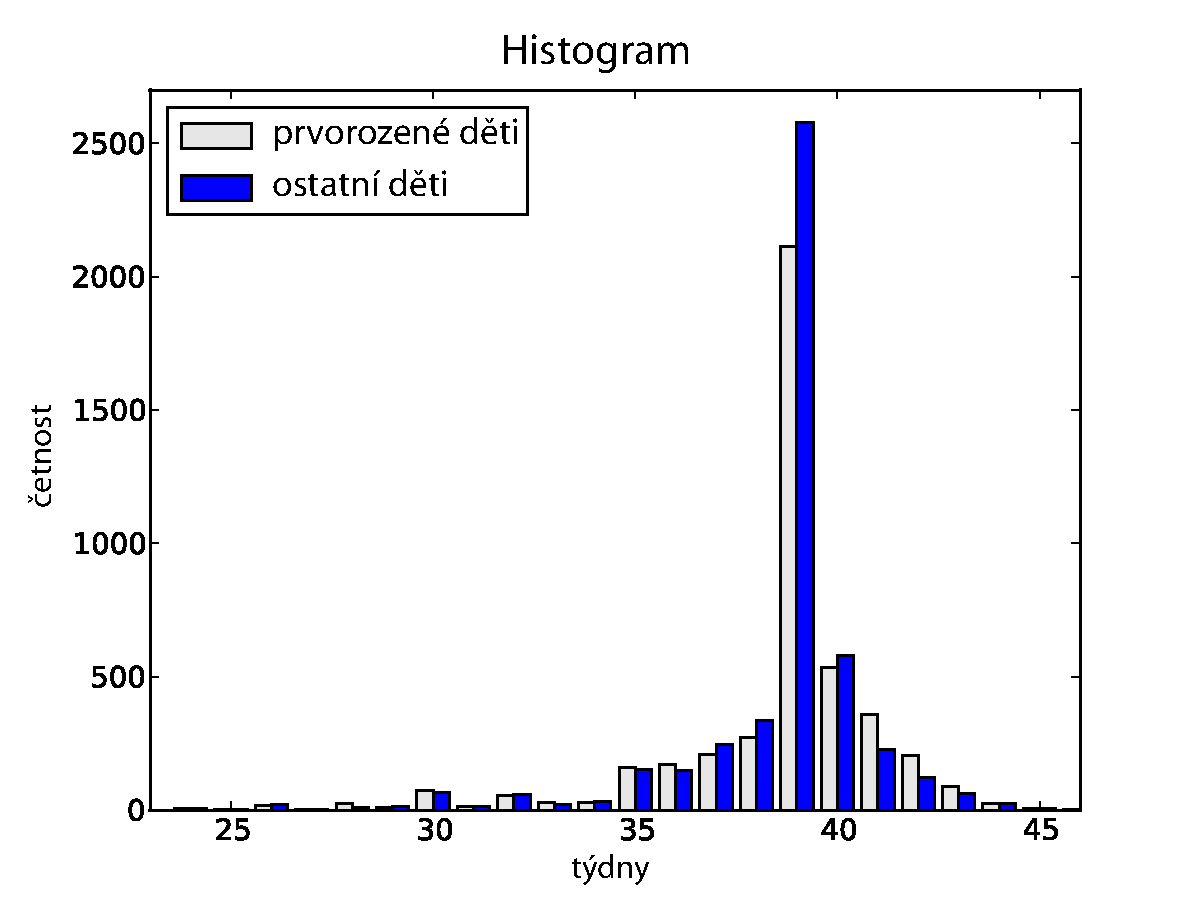
\includegraphics[height=2.5in]{figs/nsfg_hist.pdf}}
\caption{Histogram délek těhotenství.}
\label{nsfg_hist}
\end{figure}

Histogramy jsou užitečné, protože jsou z nich bezprostředně patrné následující vlastnosti:

\begin{description}

\item[Modus:] Nejčastěji se vyskytující hodnota v rozdělení se nazývá
  {\bf modus}.  Na obrázku~\ref{nsfg_hist} je zřejmý modus v 39. týdnu.  V tomto případě je modus souhrnnou statistickou charakteristikou, která nejlépe vystihuje typickou hodnotu.
 \index{modus}

\item[Tvar:] Kolem modu je rozdělení asymetrické; napravo klesá rychle, zatímco nalevo je pokles pomalejší. Z medicínského hlediska to dává smysl. Děti se často narodí předčasně, ale zřídka později než ve 42. týdnu. Pravá strana rozdělení
je však useknutá také kvůli tomu, že doktoři často po 42. týdnu zasáhnou.
  \index{tvar}

\item[Odlehlé hodnoty:] Hodnoty vzdálené od modu se nazývají {\bf odlehlé hodnoty}.
  Některé z nich představují neobvyklé případy, jako například děti narozené v 30. týdnu.
 Mnohé z nich jsou ale způsobeny chybami, k nimž dojde při vykazování nebo zaznamenávání dat.
\index{odlehlá hodnota}

\end{description}

Přestože histogramy ozřejmí některé vlastnosti, obvykle se nedají příliš dobře použít pro
srovnání dvou rozdělení. V tomto příkladu je  méně ``prvorozených'' než ``ostatních'' dětí,
a tak jsou některé zjevné rozdíly v histogramech způsobeny rozsahem výběru. Tento problém můžeme
vyřešit pomocí pravděpodobnostních funkcí (PMFs).


\section{\protect\raggedright Zobrazování pravděpodobnostních funkcí (PMFs)}
\index{Pmf objekt}
\index{{\tt pmf.py}@{\tt Pmf.py}}

{\tt Pmf.py} poskytuje třídu s názvem {\tt Pmf}, která zobrazuje pravděpodobnostní
funkce (PMFs). Její zápis může být matoucí, ale je opravdu takovýto: {\tt Pmf} je název
modulu a také název třídy, takže celý název třídy je {\tt Pmf.Pmf}.  Často používám {\tt pmf} jako název proměnné.
Konečně pak v textu používám zkratku PMF pro označení obecného konceptu pravděpodobnostní
funkce (probability mass function), nezávisle na mém způsobu implementace.

Pro vytvoření Pmf objektu, použijte {\tt MakePmfFromList}, která přijme seznam
hodnot:
%
\begin{verbatim}
>>> import Pmf
>>> pmf = Pmf.MakePmfFromList([1, 2, 2, 3, 5])
>>> print pmf
<Pmf.Pmf object at 0xb76cf68c>
\end{verbatim}

Pmf a Hist objekty si jsou v mnoha ohledech podobné. Metody {\tt
  Values} a {\tt Items} fungují stejně pro oba typy.  Největší rozdíl je v tom, že Hist přiřadí k
  hodnotám počitadla celých čísel, zatímco Pmf přiřadí k hodnotám pravděpodobnosti v režimu pohyblivé řádové čárky.

K vyhledání pravděpodobnosti spojené s konkrétní hodnotou, použijte {\tt Prob}:
%
\begin{verbatim}
>>> pmf.Prob(2)
0.4
\end{verbatim}

Stávající Pmf můžete modifikovat zvýšením pravděpodobnosti spojené s hodnotou:
%
\begin{verbatim}
>>> pmf.Incr(2, 0.2)
>>> pmf.Prob(2)
0.6
\end{verbatim}

Nebo můžete pravděpodobnost vynásobit činitelem:
%
\begin{verbatim}
>>> pmf.Mult(2, 0.5)
>>> pmf.Prob(2)
0.3
\end{verbatim}

Jestliže modifikujete Pmf, výsledek nemusí být normalizovaný, tzn. že pravděpodobnosti již nemusí být v součtu
rovny 1.  Pro kontrolu můžete volat {\tt
  Total}, která vrátí součet pravděpodobností:
%
\begin{verbatim}
>>> pmf.Total()
0.9
\end{verbatim}

Pro renormalizaci volejte {\tt Normalize}:
%
\begin{verbatim}
>>> pmf.Normalize()
>>> pmf.Total()
1.0
\end{verbatim}

Pmf objekty umožňují metodu {\tt Copy}, takže si můžete vytvořit a modifikovat kopii, aniž by tím byl
dotčen originál.

\begin{exercise}
Jak uvádí Wikipedie: ``Analýza přežití je statistická disciplína, která se zabývá smrtí
biologických organismů a selháním mechanických systémů;'' viz \url{http://wikipedia.org/wiki/Survival_analysis}.
\index{analýza přežití}

V rámci analýzy přežití je často užitečné vypočíst např. zůstatkovou životnost mechanické součástky.
Pokud známe rozdělení životností a stáří součástky, jsme schopni spočítat rozdělení zůstatkových životností.

Napište funkci nazvanou {\tt RemainingLifetime}, která přijme Pmf životností a věku a vrátí novou
Pmf, která zobrazuje rozdělení zůstatkových životností.

\end{exercise}


\begin{exercise}
%
\index{průměr}
\index{rozptyl}
\index{PMF}
%
V Oddílu ~\ref{mean} jsme spočítali průměr výběru sečtením prvků a vydělením
 \n.  Jestliže znáte PMF, můžete stále vypočítat průměr, ovšem postup bude trochu jiný:
%
\[ \mu = \sum_i p_i x_i \]
%
kde \xsubi~jsou jedinečné hodnoty v PMF a \psubi=PMF(\xsubi).
Obdobně můžete vypočíst rozptyl pomocí následujícícho vzorce:
%
\[ \sigma^2 = \sum_i p_i (x_i - \mu)^2\]
%
Napište funkce nazvané {\tt PmfMean} a {\tt PmfVar}, které přijmou
Pmf objekt a vypočtou průměr a rozptyl. K otestování těchto metod
zkontrolujte, jestli jsou konzistentní s metodami {\tt Mean} a {\tt
  Var} v {\tt Pmf.py}.
\index{{\tt pmf.py}@{\tt Pmf.py}}

\end{exercise}




\section{\protect\raggedright Grafické znázornění pravděpodobnostních funkcí (PMFs)}
\index{grafické znázornění}
\index{PMF}

Běžně se můžeme setkat se dvěma způsoby grafického znázornění PMFs:

\begin{itemize}

\item Pro znázornění Pmf pomocí sloupcového grafu můžete použít {\tt pyplot.bar}
nebo {\tt myplot.Hist}. Sloupcové grafy se nejlépe hodí, jestliže jsou číslo nebo hodnoty v
Pmf malé.
\index{sloupcový graf}
\index{graf!sloupcový}

\item Pro znázornění Pmf  jako přímky můžete použít {\tt pyplot.plot}
nebo {\tt myplot.Pmf}.  Spojnicové grafy jsou nejvhodnější, jestliže máme velké množství
hodnot a Pmf je vyrovnaná.
\index{spojnicový graf}
\index{graf!spojnicový}

\end{itemize}

\begin{figure}
% descriptive.py
\centerline{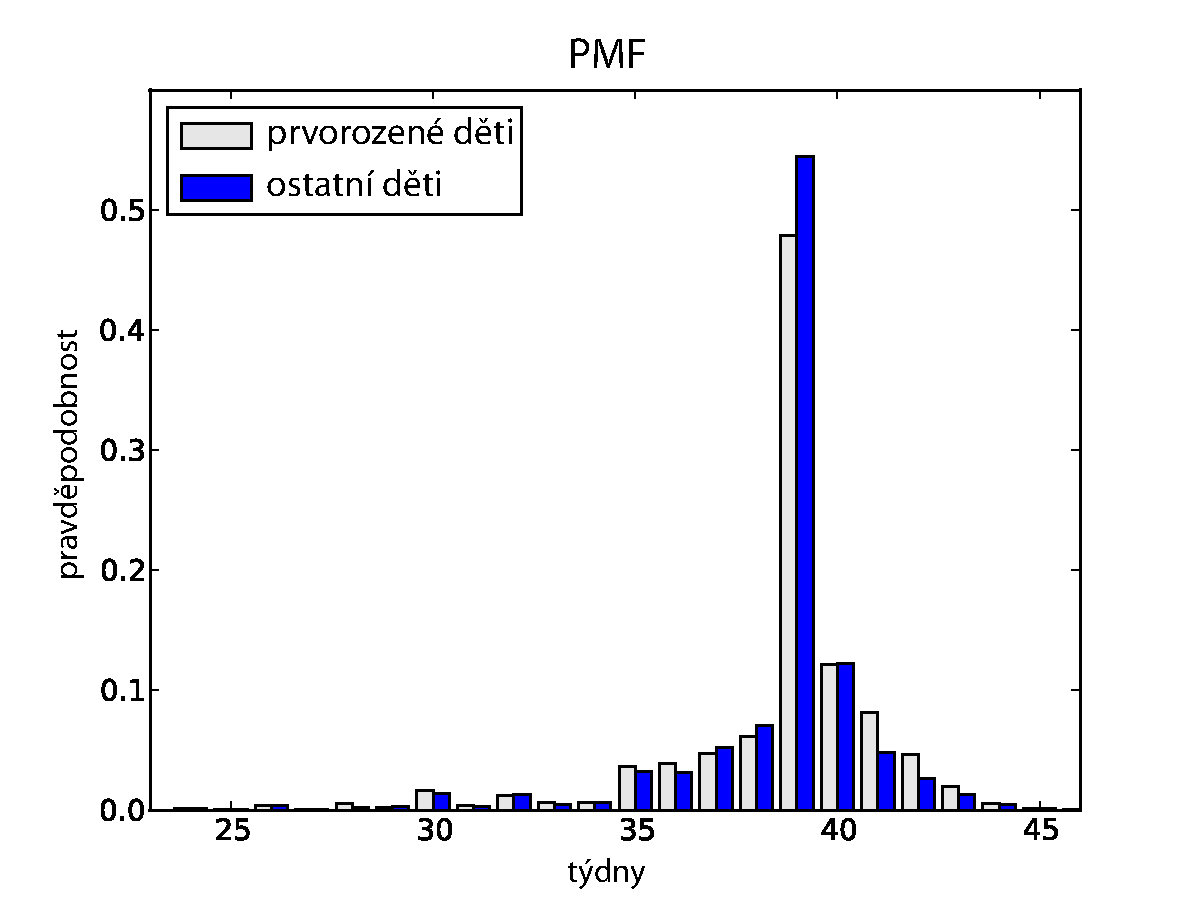
\includegraphics[height=2.5in]{figs/nsfg_pmf.pdf}}
\caption{PMF délek těhotenství.}
\label{nsfg_pmf}
\end{figure}
\index{délka těhotenství}

Obrázek~\ref{nsfg_pmf} ukazuje PMF délek těhotenství jako sloupcový graf.
Prostřednictvím PMF jsme schopni zřetelněji vidět, kde se rozdělení liší.
Zdá se, že u prvorozených dětí je menší pravděpodobnost, že se narodí načas (v 39. týdnu)
a větší pravděpodobnost, že se narodí se zpožděním (v 41. a 42. týdnu).

Kód generující obrázky v této kapitole je dostupný na
\url{http://thinkstats.com/descriptive.py}.  K jeho spuštění budete potřebovat moduly,
které importuje, a data z NSFG (viz
Oddíl~\ref{nsfg}).
\index{Národní šetření růstu rodin -- National Survey of Family Growth}
\index{NSFG}
\index{{\tt descriptive.py}}

Poznámka: {\tt pyplot} umožňuje funkci nazvanou {\tt hist}, která přijme posloupnost
hodnot, spočítá histogram a graficky jej znázorní. Protože používám {\tt Hist} objekty, obvykle
nepoužívám {\tt pyplot.hist}.


\section{\protect\raggedright Odlehlé hodnoty}
\index{odlehlá hodnota}

Odlehlé hodnoty jsou hodnoty, které jsou vzdálené od střední hodnoty.  Odlehlé hodnoty
mohou být způsobeny chybami při sběru nebo zpracování dat, nebo se může jednat o správné ale neobvyklé
výsledky měření. Je vždy rozumné provést kontrolu s ohledem na odlehlé hodnoty a přitom je někdy také užitečné
a vhodné je odstranit.

%weeks  count
%0      1
%4      1
%9      1
%13     1
%17     2
%18     1
%19     1
%20     1
%21     2
%22     7

V seznamu délek těhotenství pro porody živého dítěte je následujících 10 nejnižších
hodnot \{0, 4, 9, 13, 17, 17, 18, 19, 20, 21\}.  Hodnoty pod 20 týdnů
jsou zcela jistě chyby, hodnoty nad 30 týdnů jsou pravděpodobně legitimní.
Avšak hodnoty mezi tím se těžko interpretují.
\index{délka těhotenství}

Naproti tomu nejvyšší hodnoty jsou následující:
%
\begin{verbatim}
weeks  count
43     148
44     46
45     10
46     1
47     1
48     7
50     2
\end{verbatim}

Opět platí, že některé hodnoty jsou téměř jistě chyby, není ale snadné získat
o tom absolutní jistotu. Jednou možností je provést {\bf ořezání} dat
tím, že odstraníme část nejvyšších a nejnižších hodnot (viz
\url{http://wikipedia.org/wiki/Truncated_mean}).
\index{oříznutý průměr}
\index{průměr!oříznutý}
\index{useknutý průměr}
\index{průměr!useknutý}


\section{\protect\raggedright Další vizualizace}
\index{vizualizace}
\index{explorační analýza dat}

Histogramy a pravděpodobnostní funkce (PMFs) se hodí pro explorační analýzu dat; jakmile máte představu o tom, co se děje,
je často užitečné navrhnout vizualizaci, která se zaměří na pozorované zjištění.
\index{pozorované zjištění}

V rámci dat NSFG se největší rozdíly v rozdělení objevují blízko modu.
Má proto smysl přiblížit si tuto část grafu a provést transformaci dat ke zvýraznění rozdílů.
\index{Národní šetření růstu rodin -- National Survey of Family Growth}
\index{NSFG}

Obrázek~\ref{nsfg_diffs} ukazuje rozdíl mezi PMFs pro týdny
35--45.  Provedl jsem násobení 100, abychom získali rozdíly v procentních
bodech.

\begin{figure}
% descriptive.py
\centerline{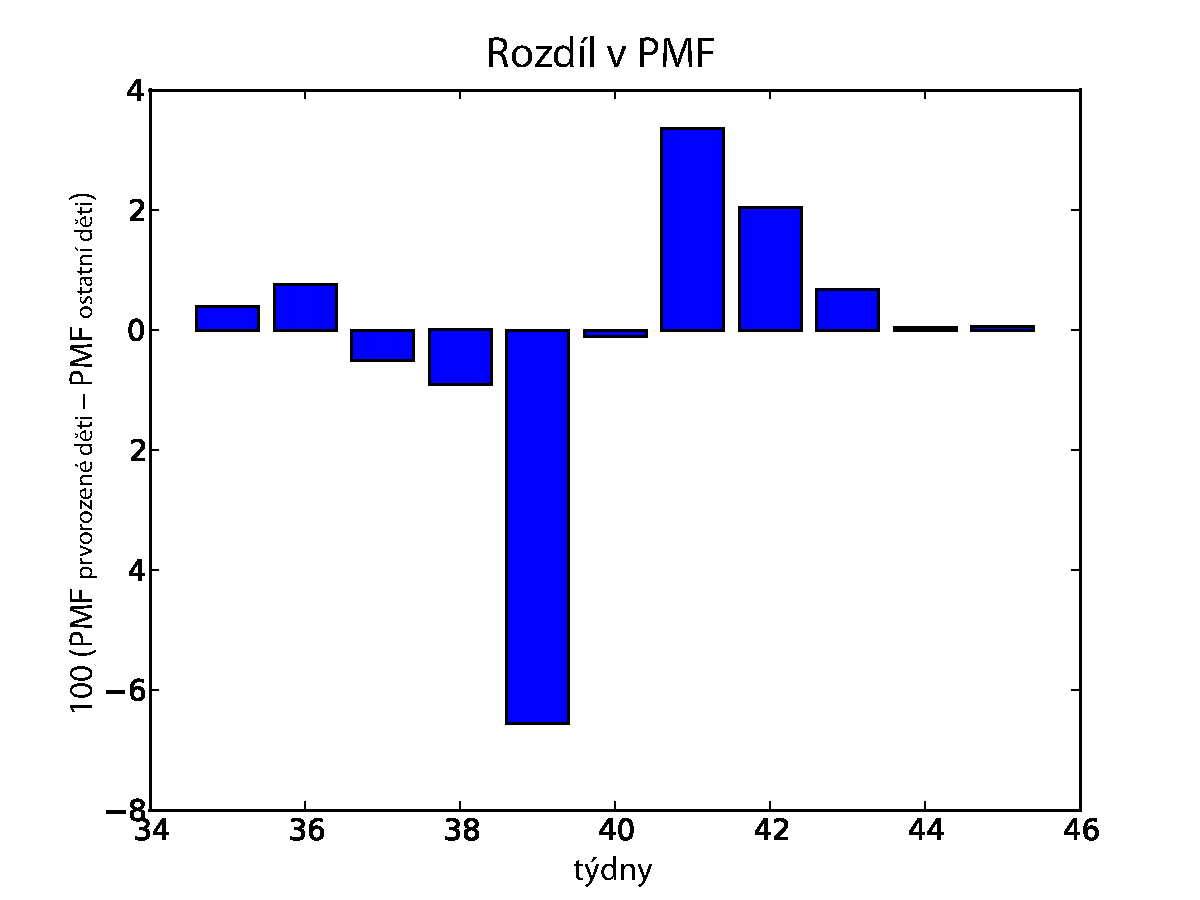
\includegraphics[height=2.5in]{figs/nsfg_diffs.pdf}}
\caption{Rozdíl v procentech, po týdnech.}
\label{nsfg_diffs}
\end{figure}

Na tomto obrázku je dobře patrný vzor: u prvorozených dětí je menší pravděpodobnost, že
se narodí v 39. týdnu, a poněkud větší pravděpodobnost jejich narození v 41. nebo 42. týdnu.


\section{\protect\raggedright Relativní riziko}
\label{relative.risk}
\index{relativní riziko}

Začali jsme otázkou: ``Rodí se prvorozené děti se zpožděním?''  Abychom to trochu upřesnili,
řekněme, že dítě se narodí předčasně, pokud přijde na svět v průběhu 37. týdne nebo dříve, načas, pokud
se narodí v průběhu 38., 39. nebo 40. týdne, a se zpožděním, pokud se narodí v průběhu
41. týdne nebo později. Rozpětí jako tato, která se používají k seskupování dat, se nazývají {\bf třídy}.
\index{třída}
\index{{\tt risk.py}}

\begin{exercise}
Vytvořte soubor s názvem {\tt risk.py}.
Napište funkce nazvané {\tt ProbEarly}, {\tt ProbOnTime} a
{\tt ProbLate}, které přijmou PMF a vypočítají podíl narození, která spadají do jednotlivých tříd. Nápověda:
Napište zobecněnou funkci, kterou tyto funkce volají.

Vytvořte tři PMFs, jednu pro prvorozené děti, jednu pro ostatní a jednu pro všechny
porody živých dětí. Pro každou PMF vypočtěte pravděpodobnost předčasného narození,
narození načas a narození se zpožděním.

Jedním ze způsobů jak sumarizovat takováto data je pomocí {\bf relativního rizika},
které představuje poměr dvou pravděpodobností. Například pravděpodobnost, že se prvorozené
dítě narodí předčasně, je 18,2 \%.  Pro ostatní děti je tato pravděpodobnost
16,8 \% a relativní riziko je tedy 1,08.  To znamená, že u prvorozených dětí je přibližně o 8 \% větší
pravděpodobnost, že se narodí předčasně.

Napište kód, který potvrdí tento výsledek, a poté vypočtěte relativní riziko předčasného narození a
narození se zpožděním. Řešení si můžete stáhnout z \url{http://thinkstats.com/risk.py}.

\end{exercise}


\section{\protect\raggedright Podmíněná pravděpodobnost}
\index{podmíněná pravděpodobnost}
\index{pravděpodobnost!podmíněná}

Představte si, že nějaká vaše známá je těhotná a právě začíná 39. týden jejího těhotenství.
Jaká je šance, že se dítě narodí v následujícím týdnu? Jak se odpověď změní, jestliže se jedná o
první dítě?

Odpověď na tuto otázku můžeme najít prostřednictvím výpočtu {\bf podmíněné pravděpodobnosti}, což je (ehm!) pravděpodobnost, která závisí na podmínce.
V tomto případě je touto podmínkou skutečnost, že víme, že se dítě nenarodilo v 0.--38. týdnu.

Zde je jeden způsob, jak to provést:

\begin{enumerate}

\item Na základě známé PMF vytvořte falešnou kohortu o 1000 těhotenstvích.
Pro každý počet týdnů, \x, je počet těhotenství s délkou \x~
1000 PMF(\x).
\index{kohorta}

\item Z kohorty odstraňte všechna těhotenství, která trvají méně než 39 týdnů.
\index{délka těhotenství}

\item Vypočtěte PMF zbývajících délek; výsledkem je podmíněná PMF.

\item Vypočtěte podmíněnou PMF, jestliže \x~=~39 týdnů.

\end{enumerate}

Tento algoritmus je koncepčně jasný, ale není příliš účinný.
Jednoduchou alternativou je odstranit z rozdělení hodnoty pod 39 a pak provést
renormalizaci.

\begin{exercise}
Napište funkci, která uplatní kterýkoli z těchto algoritmů a vypočte pravděpodobnost, že se dítě
narodí v průběhu 39. týdne, za předpokladu, že se nenarodilo před začátkem 39. týdne.

Zobecněte tuto funkci tak, abyste vypočítali pravděpodobnost, že se dítě narodí během týdne
\x, za předpokladu, že se nenarodilo před začátkem týdne \x, a to pro všechna \x.
Proveďte grafické znázornění této hodnoty jako funkce \x~ pro prvorozené děti a ostatní.

Řešení tohoto úkolu si můžete stáhnout zde:
\url{http://thinkstats.com/conditional.py}.
\index{{\tt conditional.py}}

\end{exercise}


\section{\protect\raggedright Referování o výsledcích}

Dospěli jsme do bodu, kdy jsme prozkoumali data a zaznamenali jsme několik
pozorovaných zjištění.  Pro tuto chvíli předpokládejme, že jsou tato zjištění skutečná (nezapomeňme však, že jde o
předpoklad). Jak bychom měli o těchto výsledcích referovat?

Odpověď by se mohla odvíjet od toho, kdo otázku položil. Například vědec by se mohl zajímat
o jakýkoli (skutečný) výsledek, bez ohledu na jeho velikost. Doktor by se mohl zajímat pouze o ty výsledky,
které jsou {\bf  klinicky významné}; totiž takové, které mají vliv na rozhodnutí o léčbě. Těhotnou ženu by
mohly zajímat výsledky, které jsou pro ni relevantní, jako například podmíněné pravděpodobnosti,
jimiž jsme se zabývali v předchozí části.
\index{klinicky významný}
\index{významnost}

Způsob referování o výsledcích závisí také na vašich cílech. Jestliže se snažíte ukázat
významnost nějakého zjištění, pak byste mohli zvolit souhrnné statistické charakteristiky, jako například
relativní riziko, které zdůrazňují rozdíly. Jestliže je vaším cílem uklidnit pacienta, možná byste raději sáhli po statistických
charakteristikách, které tyto rozdíly zasadí do kontextu.

\begin{exercise}
Na základě výsledků z předešlých cvičení předpokládejte, že vás někdo požádal,
abyste shrnul/a, co jste zjistil/a o tom, jestli se prvorozené děti rodí se zpožděním.

Které souhrnné statistické charakteristiky byste použil/a, pokud byste chtěl/a dostat nějaký příběh do večerních
zpráv? A které byste použil/a, kdybyste chtěl/a uklidnit nervózního pacienta?
\index{Adams, Cecil}
\index{Straight Dope, The}

Na závěr si představte, že jste Cecil Adams, autor {\it The Straight
  Dope} (\url{http://straightdope.com}), a vaším úkolem je odpovědět na otázku: ``Rodí se prvorozené děti se zpožděním?''  Napište odstavec, kterým na tuto otázku odpovíte s pomocí výsledků z této kapitoly jasně, přesně a výstižně.

\end{exercise}



\section{\protect\raggedright Glosář}

\begin{description}

\item[centrální tendence (central tendency):] Charakteristika vzorku populace;
intuitivně se jedná o nejprůměrnější hodnotu.
\index{centrální tendence}

\item[variabilita (spread):] Charakteristika vzorku populace;
intuitivně se jedná o popis velikosti variability.
\index{variabilita}

\item[rozptyl (variance):] Souhrnná statistická charakteristika, která se často používá ke kvantifikaci variability.
\index{rozptyl}

\item[směrodatná odchylka (standard deviation):] Druhá odmocnina z rozptylu, také se používá jako míra variability.
\index{směrodatná odchylka}

\item[četnost (frequency):] Počet výskytů hodnoty ve výběrovém souboru.
\index{četnost}

\item[histogram:] Zobrazení rozložení četností jednotlivých hodnot nebo graf, který toto zobrazení znázorňuje.
\index{histogram}

\item[pravděpodobnost (probability):] Četnost vyjádřená jako podíl rozsahu výběru.
\index{pravděpodobnost}

\item[normalizace (normalization):] Proces dělení četnosti rozsahem výběru za účelem získání pravděpodobnosti.
\index{normalizace}

\item[rozdělení (distribution):] Souhrn hodnot, které se vyskytují ve výběru a četnost, nebo pravděpodobnost,
každé z nich.

\index{rozdělení}

\item[pravděpodobnostní funkce (PMF) (probability mass function):] Zobrazení rozdělení jako funkce, kde jsou hodnotám přiřazeny pravděpodobnosti.
\index{PMF}

\item[modus (mode):] Hodnota s největší četností ve výběru.
\index{modus}

\item[odlehlá hodnota (outlier):] Hodnota vzdálená od střední hodnoty.
\index{odlehlá hodnota}

\item[ořezat (trim):] Odstranit ze souboru dat odlehlé hodnoty.
\index{ořezat}

\item[třída (bin):] Rozpětí používané k seskupování hodnot, které se vyskytují blízko sebe.
\index{třída}

\item[relativní riziko (relative risk):] Poměr dvou pravděpodobností, často používaný k měření rozdílu mezi rozděleními.
\index{relativní riziko}

\item[podmíněná pravděpodobnost (conditional probability):] Pravděpodobnost vypočtená za předpokladu platnosti určité podmínky.
\index{podmíněná pravděpodobnost}

\item[klinicky významný (clinically significant):] Výsledek, jako například rozdíl mezi skupinami, který je relevantní pro praxi.
\index{klinicky významný}

\end{description}


\chapter{Distribuční funkce}
\label{cumulative}

\section{\protect\raggedright Paradox počtu studentů v kurzu}
\index{počet studentů v kurzu}

Na řadě amerických vysokých škol a univerzit je poměr studentů k fakultnímu sboru 10:1.  Studenti jsou však často překvapeni, když zjistí, že průměrný počet studentů v kurzu je větší než 10. Za touto nesrovnalostí stojí dva důvody:

\begin{itemize}

\item Studenti si obvykle zvolí 4--5 kurzů za semestr, ale učitelé často učí pouze 1 nebo 2 kurzy.

\item Není mnoho studentů, kteří by si libovali v kurzech, do kterých je zapsáno málo studentů, ale počet studentů v kurzu, který si zvolí velké množství studentů, je (ehm!) velký.

\end{itemize}

První efekt je zřejmý (minimálně poté, co je na něj poukázáno), zatímco ten druhý
tak evidentní není.  Podívejme se tedy na příklad. Předpokládejme, že vysoká škola nabízí v rámci jednoho semestru 65 kurzů, přičemž jejich rozdělení podle počtu studentů v kurzu (velikosti kurzu) je následující:
%
\begin{verbatim}
 velikost     počet
 5- 9          8
10-14          8
15-19         14
20-24          4
25-29          6
30-34         12
35-39          8
40-44          3
45-49          2
\end{verbatim}

Pokud se zeptáte na průměrný počet studentů v kurzu děkana, bude postupovat tak, že stanoví PMF, vypočte průměr a uvede, že průměrný počet studentů v kurzu je 24.

Pokud se ale budete dotazovat skupiny studentů na to, kolik studentů je v jejich kurzu, a vypočtete průměr, pak dospějete k závěru, že průměrný počet studentů v kurzu je větší.

\begin{exercise}
Určete PMF těchto dat a vypočtěte průměr z pohledu děkana. Vzhledem k tomu, že data byla uspořádána do tříd, můžete použít střed každé třídy.
\index{PMF}

Nyní zjistěte rozdělení počtu studentů v kurzu z pohledu studentů a vypočtěte průměr.

Předpokládejme, že chcete zjistit rozdělení počtu studentů v kurzech na vysoké škole, ale nemůžete získat spolehlivá data od děkana. Alternativou je vybrat náhodný vzorek studentů a zeptat se jich na počet studentů v každém z kurzů, který navštěvují. Pak můžete vypočíst PMF na základě jejich odpovědí.
\index{zkreslení!nadreprezentování}
\index{nadreprezentování}

Výsledek by byl zkreslený nadreprezentováním kurzů s větším počtem studentů, ale skutečné rozdělení počtu studentů v kurzech byste mohli odhadnout na základě vhodné transformace pozorovaného rozdělení.

Napište funkci nazvanou \verb"UnbiasPmf", která přijme PMF pozorovaných hodnot a vrátí nový
Pmf objekt, který vyjadřuje odhad rozdělení počtu studentů v kurzech.

Řešení tohoto problému si můžete stáhnout na
\url{http://thinkstats.com/class_size.py}.
\index{{\tt class\_size.py}}

\end{exercise}


\begin{exercise}
\label{relay}

Ve většině běžeckých závodů startují všichni účastníci zároveň.  Jestliže máte rychlé tempo, pak obvykle na začátku závodu předběhnete spoustu lidí, ale po několika mílích už běží všichni kolem vás zhruba stejnou rychlostí.
\index{štafetový závod}
\index{zkreslení!nadreprezentování}
\index{nadreprezentování}

Když jsem běžel dálkový štafetový závod (209 mílí) poprvé, všiml jsem si zvláštního jevu: Když jsem předběhl jiného běžce, byl jsem obvykle výrazně rychlejší, a když jiný běžec předběhl mě, byl obvykle výrazně rychlejší.

Nejdřív jsem si myslel, že rozdělení rychlostí by mohlo být bimodální, totiž že se závodu účastnilo hodně pomalých běžců a hodně rychlých běžců, ale málo běžců s podobnou rychlostí, jakou běhám já.

Pak jsem si uvědomil, že jsem se stal obětí zkreslení výběru. Závod byl neobvyklý hned ve dvou ohledech: Jednak se startovalo postupně, takže jednotlivé týmy začínaly různě, a jednak byla řada týmů složená z běžců na různé úrovni.
\index{zkreslení!selektivní}
\index{selektivní zkreslení}

Ve výsledku tak byli jednotliví běžci rozptýleni po trati, přičemž mezi jejich rychlostí a místem, kde se nacházeli, nebyl žádný jednoznačný vztah. Když jsem zahájil svůj úsek, představovali běžci kolem mě (do velké míry) náhodný vzorek běžců účastnících se závodu.

Odkud se tedy bere to zkreslení?  V době, kdy běžím na trati závodu, je pravděpodobnost, že předběhnu jiného běžce nebo že on předběhne mě, proporcionální k rozdílu v našich rychlostech. Abyste si uvědomili, proč tomu tak je, zamyslete se nad extrémy. Jestliže jiný běžec běží stejně rychle jako já, pak ani jeden z nás nepředběhne toho druhého. Jestliže někdo běží tak rychle, že za dobu, kdy já běžím, uběhne celou trať závodu, pak je jisté, že mě takový běžec předběhne.

Napište funkci nazvanou {\tt BiasPmf}, která přijme Pmf představující skutečné rozdělení rychlostí běžců a rychlost běžícího pozorovatele a vrátí novou Pmf představující rozdělení rychlostí běžců, jak je vnímá pozorovatel.

K otestování vaší funkce získejte rozdělení rychlostí z normálního běžeckého závodu (ne štafety).
Vytvořil jsem program, který přečte výsledky závodu James Joyce Ramble 10K v Dedhamu ve státě Massachusetts a převede tempo každého běžce na míle za hodinu (MPH). Stáhněte si jej z:
\url{http://thinkstats.com/relay.py}.  Spusťte jej a podívejte se na PMF rychlostí.
\index{{\tt relay.py}}
\index{{\tt relay\_soln.py}}

Nyní vypočtěte rozdělení rychlostí, jaké byste pozoroval/a, pokud byste běžel/a štafetový závod rychlostí
7,5 MPH s touto skupinou běžců.  Řešení si můžete stáhnout na: \url{http://thinkstats.com/relay_soln.py}

\end{exercise}


\section{\protect\raggedright Limity pravděpodobnostních funkcí (PMFs)}
\index{PMF}

Pravděpodobnostní funkce fungují dobře při malém počtu hodnot. Jakmile ale počet hodnot stoupne, pravděpodobnost spojená s každou z hodnot se sníží a narůstá vliv náhodného šumu.

Mohli bychom se například zajímat o rozdělení porodních hmotností.  V rámci souboru dat NSFG je proměnná \verb"totalwgt_oz" záznamem váhy při narození vyjádřené v uncích.
Obrázek~\ref{nsfg_birthwgt_pmf} znázorňuje PMF těchto hodnot pro prvorozené děti a ostatní.
\index{Národní šetření růstu rodin -- National Survey of Family Growth}
\index{NSFG}
\index{porodní hmotnost}
\index{hmotnost!porodní}

\begin{figure}
% cumulative.py
\centerline{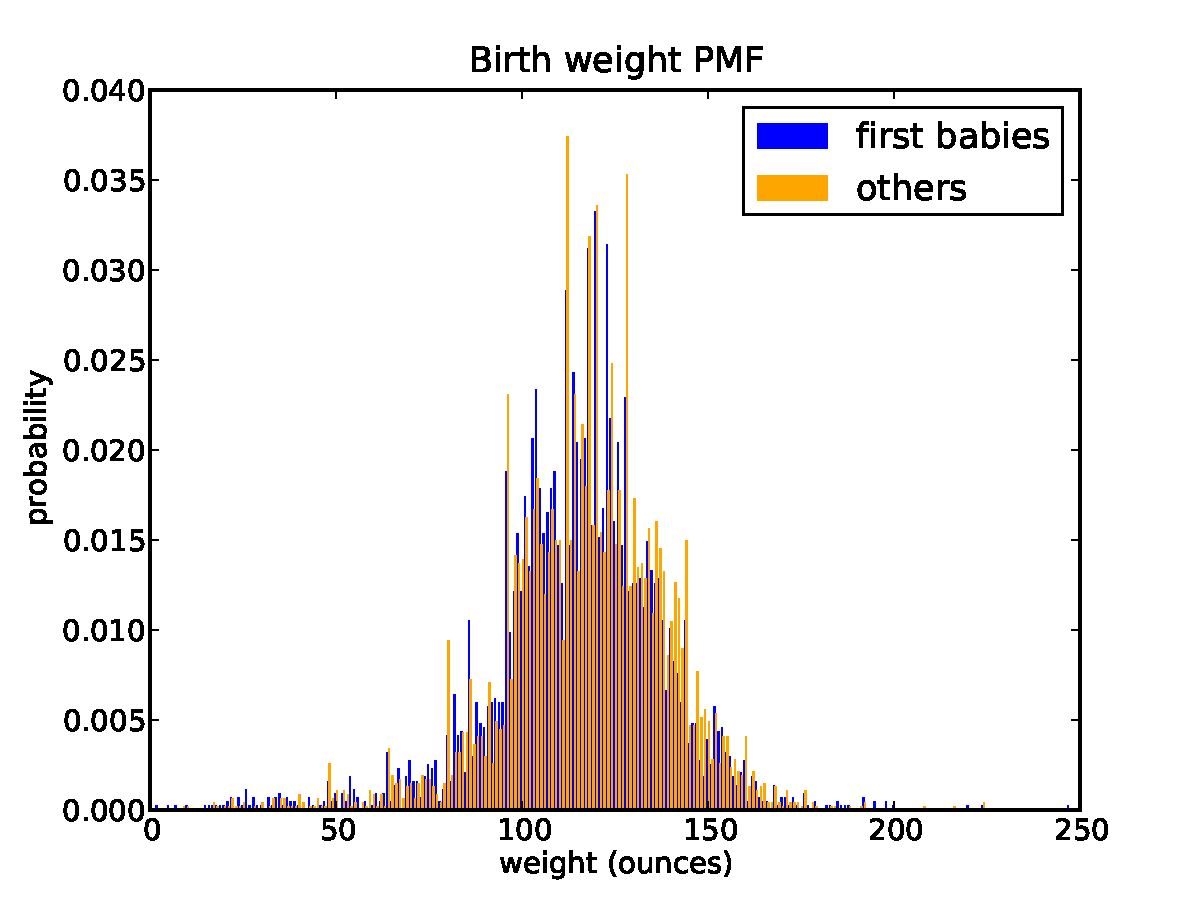
\includegraphics[height=2.5in]{figs/nsfg_birthwgt_pmf.pdf}}
\caption{PMF porodních hmotností.  Tento obrázek znázorňuje omezení PMFs:
obtížně se porovnávají.}
\label{nsfg_birthwgt_pmf}
\end{figure}

Celkově připomínají tato rozdělení známé ``normální rozdělení'' s velkým počtem hodnot blízko průměru a malým počtem hodnot o mnoho výše nebo níže.

Části tohoto grafu se ale obtížně interpretují. Je tam velké množství prudkých vzestupů a propadů a některé zjevné rozdíly mezi rozděleními. Je obtížné určit, které z těchto rysů jsou významné. Také není snadné identifikovat celkové vzory. Například které rozdělení má podle vás vyšší průměr?
\index{rozdělení do tříd}

Tyto problémy je možné zmírnit tím, že data uspořádáme do tříd, tedy rozdělíme oblast hodnot do intervalů, které se vzájemně nepřekrývají, a spočítáme počet hodnot v každé třídě. Rozdělení do tříd může být užitečné, ale není vůbec snadné správně nastavit velikost tříd. Budou-li dostatečně velké, aby odfiltrovaly šum, pak mohou zároveň odfiltrovat také užitečné informace.

Alternativou, která se těmto problémům vyhne, je {\bf distribuční
funkce} označovaná také jako {\bf CDF}.  Než se k ní ale dostaneme, je potřeba se podívat na percentily.
\index{distribuční funkce}
\index{CDF}


\section{\protect\raggedright Percentily}
\index{percentilové pořadí}

Pokud jste vykonali nějaký standardizovaný test, pravděpodobně jste obdrželi výsledky ve formě hrubého skóre a {\bf percentilového pořadí}.
V tomto kontextu představuje percentilové pořadí podíl osob, které dosáhly horšího výsledku než vy (nebo stejného). Takže pokud jste se umístili v ``90. percentilu,'' dosáhli jste stejného nebo lepšího výsledku než 90 \% všech, kdo zkoušku vykonali.


Zde je postup, jak můžete vypočítat percentilové pořadí hodnoty,
\verb"your_score", relativně vůči skóre v rámci řady {\tt
  skóre}:
%
\begin{verbatim}
def PercentileRank(scores, your_score):
    count = 0
    for score in scores:
        if score <= your_score:
            count += 1

    percentile_rank = 100.0 * count / len(scores)
    return percentile_rank
\end{verbatim}
%
% see score_example.py
%
Například jestliže by skóre v řadě byla 55, 66, 77, 88 a 99
a vy byste dosáhl/a výsledku 88, pak by vaše percentilové pořadí bylo {\tt 100 * 4 / 5}, tedy
80.

Jestliže máte hodnotu, pak je snadné zjistit její percentilové pořadí, opačný postup je o něco obtížnější. Znáte-li percentilové pořadí a chcete zjistit odpovídající hodnotu, jednou z možností je uspořádat hodnoty a hledat tu, kterou chcete zjistit:
%
\begin{verbatim}
def Percentile(scores, percentile_rank):
    scores.sort()
    for score in scores:
        if PercentileRank(scores, score) >= percentile_rank:
            return score
\end{verbatim}

Výsledkem tohoto výpočtu je {\bf percentil}.  Například 50. percentil je hodnota s percentilovým pořadím 50. V rozdělení výsledků zkoušky odpovídá 50. percentilu hodnota 77.
\index{percentil}

\begin{exercise}
Tento způsob využití {\tt Percentile} není příliš efektivní.  Lepší postup je použít percentilové pořadí k výpočtu indexu odpovídajícího percentilu. Napište verzi
{\tt Percentile}, která využívá tohoto algoritmu.

Řešení si můžete stáhnout z \url{http://thinkstats.com/score_example.py}.
\index{{\tt score\_example.py}}

\end{exercise}

\begin{exercise}
Volitelné: Pokud chcete vypočíst pouze jeden percentil, pak setřídění skóre příliš nepomůže. Lepší možností je zvolit selekční algoritmus, o kterém si můžete přečíst na
\url{http://wikipedia.org/wiki/Selection_algorithm}.
\index{selekční algoritmus}

Vytvořte (nebo najděte) provedení selekčního algoritmu a použijte jej k napsání efektivní verze {\tt Percentile}.

\end{exercise}


\section{\protect\raggedright Distribuční funkce}
\index{distribuční funkce}
\index{CDF}

Teď, když už rozumíme percentilům, jsme připraveni začít se zabývat distribuční funkcí
(CDF).  Distribuční funkce (CDF) je funkce, která hodnotám přiřazuje jejich percentilové pořadí v rámci rozdělení.

CDF je funkcí \x, kde \x~je jakákoliv hodnota, která se může vyskytnout v rozdělení.
Abychom získali CDF(\x) konkrétní hodnoty \x, vypočteme podíl hodnot ve výběru, které jsou menší (nebo rovné) \x.

Zde je vyjádření téhož jako funkce, která přijme výběr {\tt t} a hodnotu {\tt x}:
%
\begin{verbatim}
def Cdf(t, x):
    count = 0.0
    for value in t:
        if value <= x:
            count += 1.0

    prob = count / len(t)
    return prob
\end{verbatim}

Tato funkce by vám měla připadat povědomá; je téměř identická s {\tt
  PercentileRank}, až na to, že výsledkem je pravděpodobnost v rozpětí 0--1, namísto percentilového pořadí v rozpětí 0--100.

Jako příklad předpokládejme, že výběr je tvořen hodnotami \{1, 2, 2, 3, 5\}.
Zde je několik hodnot z jeho distribuční funkce (CDF):

\Eqn{ CDF(0)~=~0  }

\Eqn{ CDF(1)~=~0,2 }

\Eqn{ CDF(2)~=~0,6 }

\Eqn{ CDF(3)~=~0,8 }

\Eqn{ CDF(4)~=~0,8 }

\Eqn{ CDF(5)~=~1 }

Můžeme vypočítat distribuční funkci pro jakoukoliv hodnotu, kterou může \x~nabývat, nejen hodnoty, které se vyskytují ve výběru.
Jestliže je \x~menší než nejnižší hodnota ve výběru, pak CDF(\x) je 0.
Jestliže je \x~větší než nejvyšší hodnota, pak CDF(\x) je 1.

\begin{figure}
% cumulative.py
\centerline{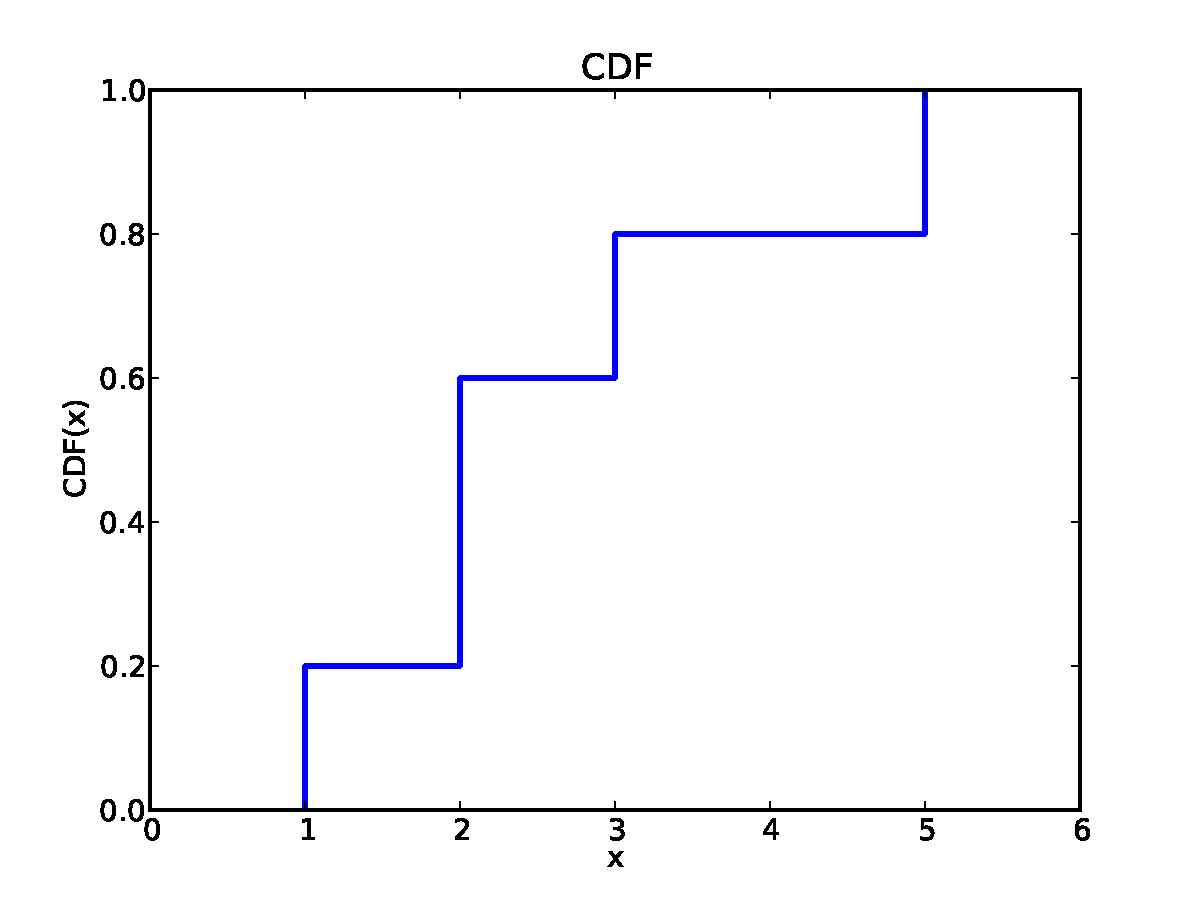
\includegraphics[height=2.5in]{figs/example_cdf.pdf}}
\caption{Příklad CDF.}
\label{example_cdf}
\end{figure}

Obrázek~\ref{example_cdf} je grafickým znázorněním této CDF.
CDF výběru je skoková funkce. V následující kapitole se zaměříme na rozdělení, jejichž distribuční funkce jsou spojité funkce.


\section{\protect\raggedright Zobrazení distribučních funkcí (CDFs)}
\index{{\tt cdf.py}@{\tt Cdf.py}}
\index{Cdf object}

Vytvořil jsem modul nazvaný {\tt Cdf}, který obsahuje třídu s názvem
{\tt Cdf}, která zobrazuje CDFs.  Dokumentaci k tomuto modulu si můžete přečíst na
\url{http://thinkstats.com/Cdf.html} a můžete si ji stáhnout zde:
\url{http://thinkstats.com/Cdf.py}.

Cdfs jsou prováděny se dvěma setříděnými seznamy: {\tt xs}, který obsahuje hodnoty, a
{\tt ps}, který obsahuje pravděpodobnosti. Nejdůležitější metody, které Cdfs nabízejí, jsou následující:

\begin{description}

\item[{\tt Prob(x)}:] Na základě hodnoty \x~vypočte pravděpodobnost \p~=~CDF(\x).

\item[{\tt Value(p)}:] Na základě pravděpodobnosti \p~vypočte odpovídající hodnotu
\x; to znamená inverzní CDF  \p.

\end{description}

Protože {\tt xs} a {\tt ps} jsou setříděné, tyto funkce mohou využít bisekční algoritmus, který je efektivní.  Doba běhu je proporcionální k logaritmu počtu hodnot; viz
 \url{http://wikipedia.org/wiki/Time_complexity}.
\index{bisekční algoritmus}

Cdfs také umožňují funkci {\tt Render}, která vrátí dva seznamy, {\tt xs} a
{\tt ps}, jež jsou vhodné ke grafickému znázornění CDF.  Protože CDF je skoková funkce, tyto seznamy obsahují dva prvky pro každou jedinečnou hodnotu v rámci rozdělení.

Modul Cdf nabízí několik funkcí pro vytváření distribučních funkcí, včetně
{\tt MakeCdfFromList}, která přijme řadu hodnot a vrátí jejich
Cdf.

Konečně pak {\tt myplot.py} skýtá funkce nazvané {\tt Cdf} a
{\tt Cdfs}, které graficky zobrazí distribuční funkce jako přímky.
\index{{\tt myplot.py}}

\begin{exercise}
Stáhněte si {\tt Cdf.py} a \verb"relay.py" (viz
Cvičení~\ref{relay}) a vygenerujte graf, který zobrazí CDF běžeckých rychlostí. Která funkce vám poskytne lepší představu o tvaru rozdělení, PMF nebo CDF? Řešení si můžete stáhnout z \url{http://thinkstats.com/relay_cdf.py}.
\index{{\tt cdf.py}@{\tt Cdf.py}}
\index{{\tt relay\_cdf.py}}

\end{exercise}


\section{\protect\raggedright Zpátky k datům z šetření}
\label{birth_weights}
\index{Národní šetření růstu rodin -- National Survey of Family Growth}
\index{NSFG}
\index{porodní hmotnost}
\index{hmotnost!porodní}

Obrázek~\ref{nsfg_birthwgt_cdf} ukazuje CDFs porodních hmotností pro prvorozené děti a ostatní v souboru dat NSFG.

\begin{figure}
% cumulative.py
\centerline{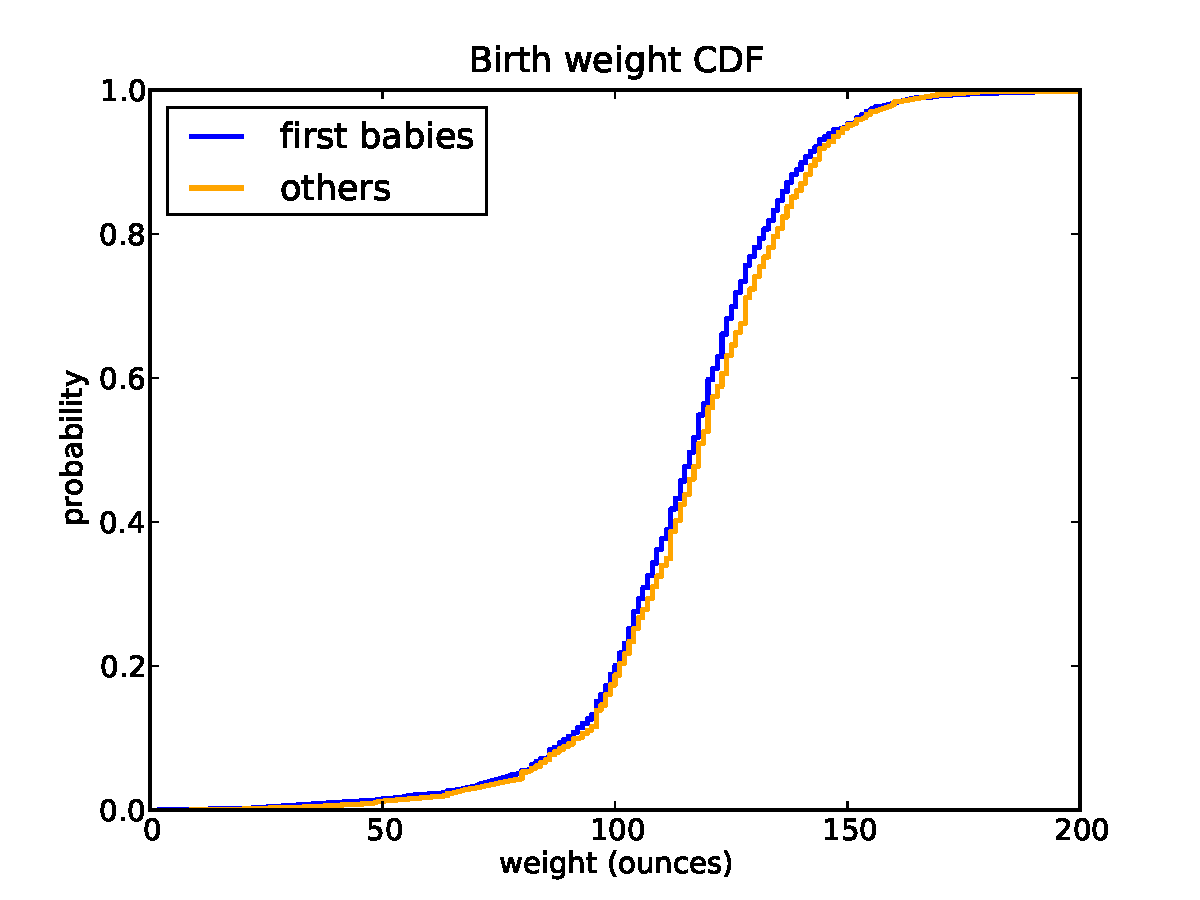
\includegraphics[height=2.5in]{figs/nsfg_birthwgt_cdf.pdf}}
\caption{CDF porodních hmotností.}
\label{nsfg_birthwgt_cdf}
\end{figure}

Díky tomuto obrázku získáme mnohem jasnější představu o tvaru rozdělení a rozdílech mezi nimi.  Je patrné, že prvorozené děti jsou mírně lehčí napříč celým rozdělením, s větší odchylkou nad průměrem.
\index{tvar}

%\begin{exercise}

%Ve výše uvedeném obrázku si můžete všimnout
%posloupnosti hodnot se stejnými rozestupy a vyšší četností než
%jejich sousedé. Zkuste přijít na to, o co jde.
%Nápověda: podívejte se na PMF \verb"birthwgt_oz".

%\end{exercise}

\begin{exercise}
Jaká byla vaše váha při narození? Pokud nevíte, zavolejte svojí matce nebo někomu jinému, kdo to ví. Za použití úhrnných dat (všechny porody živých dětí) vypočtěte rozdělení porodních hmotností a využijte je ke stanovení vašeho percentilového pořadí. Jestliže jste prvorození, zjistěte svoje percentilové pořadí v rozdělení pro prvorozené děti. Jinak použijte rozdělení pro ostatní děti. Jestliže jste v 90. percentilu nebo výše, zavolejte svojí matce a omluvte se jí.

\end{exercise}

\begin{exercise}
Předpokládejte, že spolu se svými spolužáky počítáte percentilové pořadí vašich porodních hmotností, a pak vypočtěte CDF percentilových pořadí. Jak si myslíte, že bude vypadat? Nápověda: Jaká část vaší třídy bude podle vás nad mediánem?
\index{porodní hmotnost}
\index{hmotnost!porodní}

\end{exercise}


\section{\protect\raggedright Podmíněná rozdělení}
\index{podmíněné rozdělení}
\index{rozdělení!podmíněné}

{\bf Podmíněné rozdělení} je rozdělení podmnožiny dat, která je zvolena podle určité podmínky.

Například pokud máte nadprůměrnou váhu, ale zároveň jste výrazně nadprůměrně vysoký/á, pak můžete mít relativně nízkou váhu na svoji výšku. Následuje postup, jak můžete takové tvrzení zpřesnit.

\begin{enumerate}

\item Zvolte kohortu lidí, kteří jsou stejně vysocí jako vy (v rámci určitého rozpětí).
\index{kohorta}

\item Najděte CDF hmotnosti pro tyto lidi.

\item Najděte percentilové pořadí vaší váhy v tomto rozdělení.

\end{enumerate}

Percentilová pořadí jsou užitečná pro porovnání výsledků z různých testů nebo testů použitých pro různé skupiny.
\index{percentilové pořadí}
\index{pořadí!percentilové}

Například lidé účastnící se běžeckých závodů jsou obvykle rozděleni do skupin podle věku a pohlaví. Abyste mohli porovnat osoby z různých skupin, můžete převést časy, za které závod zaběhli, na percentilová pořadí.

\begin{exercise}
Nedávno jsem běžel závod James Joyce Ramble 10K
v Denhamu ve státě Massachusetts.  Výsledky jsou dostupné na
\url{http://coolrunning.com/results/10/ma/Apr25_27thAn_set1.shtml}.
Běžte na uvedené stránky a najděte moje výsledky.  Doběhl jsem 97. mezi 1633 závodníky, takže jaké je moje percentilové pořadí mezi závodníky?
\index{James Joyce Ramble}
\index{výsledný čas závodu}

V rámci mé sekce (M4049 znamená ``muži ve věku mezi 40 a 49 lety'')
jsem doběhl 26. z 256. Jaké je moje percentilové pořadí v mé sekci?

Pokud budu za 10 let stále ještě běhat (a já doufám, že budu), budu zařazen do sekce
M5059.  Za předpokladu, že se mé percentilové pořadí v mé sekci nezmění, jaké zpomalení bych měl očekávat?

Mezi mnou a mou studentkou, která je zařazena do sekce F2039, panuje přátelská rivalita. Jak rychle by musela běžet v dalším závodě 10K, aby mě "porazila", pokud jde o percentilové pořadí?

\end{exercise}


\section{\protect\raggedright Náhodná čísla}
\label{random}
\index{náhodné číslo}

Distribuční funkce se dobře hodí pro generování náhodných čísel na základě známého rozdělení.
Podívejme se, jak se to dělá:

\begin{itemize}

\item Vyberte si náhodnou pravděpodobnost v rozpětí 0--1.

\item Použijte {\tt Cdf.Value} k nalezení hodnoty v rozdělení, jež odpovídá pravděpodobnosti, kterou jste si vybrali.

\end{itemize}

Nemusí být úplně zřejmé, proč toto funguje, ale protože je snazší to provést než vysvětlit, pojďme to zkusit.

\begin{exercise}
Napište funkci s názvem {\tt Sample}, která přijme Cdf a celé číslo \n~a vrátí seznam  \n~hodnot náhodně zvolených z Cdf.  Nápověda: Použijte {\tt random.random}.
Řešení tohoto cvičení najdete v {\tt Cdf.py}.
\index{algoritmus inverzní CDF}
\index{{\tt cdf.py}@{\tt Cdf.py}}

S využitím rozdělení porodních hmotností ze souboru NSFG vytvořte náhodný vzorek o 1000 prvcích.  Vypočtěte CDF vzorku. Sestavte graf, který zobrazuje původní CDF a CDF náhodného vzorku.  Pro velké hodnoty \n~by měla být rozdělení stejná.
\index{porodní hmotnost}
\index{hmotnost!porodní}
\index{Národní šetření růstu rodin -- National Survey of Family Growth}
\index{NSFG}

\end{exercise}

Tento proces generování náhodného vzorku na základě měřeného vzorku se nazývá {\bf resampling}.
\index{resampling}
\index{výběr}
\index{vracení, výběr}

Existují dva způsoby, jak vybrat vzorek ze souboru: s opakování nebo bez opakování. Když si představíte, že taháte koule z urny\footnote{Scénář s taháním koulí z urny představuje standardní model pro procesy náhodného výběru (viz \url{http://wikipedia.org/wiki/Urn_problem}).}, ``opakování (vracení)'' znamená, že koule v průběhu vrátíte (a zamícháte), takže soubor zůstává při každém tahu stejný. ``Bez opakování (vracení)'' znamená, že každá koule může být vytažena pouze jednou, takže zbývající soubor je po každém tahu jiný.

V Pythonu může být výběr s opakováním proveden prostřednictvím
{\tt random.random}, která provede výběr percentilového pořadí, nebo {\tt random.choice}, která slouží k výběru prvku z řady. K výběru bez opakování slouží {\tt random.sample}.
\index{modul random}

\begin{exercise}
Předpokládá se, že čísla vygenerovaná na základě {\tt random.random} budou
rovnoměrně rozdělená mezi 0 a 1, neboli že každá hodnota v rámci tohoto rozpětí bude mít stejnou pravděpodobnost.

Vytvořte 1000 čísel pomocí {\tt random.random} a graficky znázorněte jejich PMF a CDF.  Dokážete říci, jestli jsou rovnoměrně rozdělená?

O rovnoměrném rozdělení si můžete přečíst více na
\url{http://wikipedia.org/wiki/Uniform_distribution_(discrete)}.
\index{rovnoměrné rozdělení}
\index{rozdělení!rovnoměrné}

\end{exercise}


\section{\protect\raggedright Souhrnné statistické charakteristiky podruhé}
\index{souhrnná statistická charakteristika}
\index{mezikvartilové rozpětí}
\index{kvartil}
\index{percentil}
\index{medián}
\index{centrální tendence}
\index{variabilita}

Jakmile jste vypočetli CDF, je snadné vypočíst také ostatní souhrnné statistické charakteristiky. Medián je přesně 50. percentil\footnote{Můžete narazit na jiné definice mediánu. Jde zejména o to, že některé zdroje uvádějí, že jestliže máte sudý počet prvků ve výběru, je medián průměrem prostředních dvou prvků. Toto je ale zvláštní případ, který není nutné znát a který má navíc zvláštní efekt spočívající ve vytvoření hodnoty, jež není ve výběru. Pokud já vím, medián je 50. percentil. Tečka.}.
25. a 75. percentil se často používají k ověření, zda je rozdělení symetrické. Jejich rozdíl, který se nazývá {\bf mezikvartilové rozpětí}, pak měří variabilitu.

\begin{exercise}
Napište funkci s názvem {\tt Median}, která přijme Cdf a vypočte medián, a funkci nazvanou
{\tt Interquartile}, která vypočte mezikvartilové rozpětí.

Vypočtěte 25., 50. a 75. percentil CDF porodních hmotností.  Naznačují tyto hodnoty, že se jedná o symetrickou distribuci?
\index{symetrický}
\index{porodní hmotnost}
\index{hmotnost!porodní}

\end{exercise}


\section{\protect\raggedright Glosář}

\begin{description}

\item[percentilové pořadí (percentile rank):] Procento hodnot v rozdělení, které jsou menší nebo rovné určené hodnotě.
\index{percentilové pořadí}

\item[distribuční funkce (CDF) (cumulative distribution function):] Funkce, která přiděluje hodnotám jejich percentilové pořadí.
\index{CDF}

\item[percentil (percentile):] Hodnota spojená s konkrétním percentilovým pořadím.
\index{percentil}

\item[podmíněné rozdělení (conditional distribution):] Rozdělení vypočtené na základě platnosti určité podmínky.  \index{podmíněné rozdělení}

\item[resampling:] Proces generování náhodného výběru z rozdělení, které bylo vypočteno z výběru.
\index{resampling}

\item[opakování, vracení (replacement):] Při pořizování výběru znamená ``opakování'' to, že soubor je při každém výběru stejný. ``Bez opakování'' znamená, že každý prvek může být vybrán pouze jednou.
\index{opakování}

\item[mezikvartilové rozpětí (interquartile range):] Míra variability, rozdíl mezi 75. a 25. percentilem.
\index{mezikvartilové rozpětí}

\end{description}



\chapter{Spojitá rozdělení}
\label{continuous}
\index{spojité rozdělení}
\index{rozdělení!spojité}
\index{empirické rozdělení}
\index{rozdělení!empirické}

Rozdělení, s nimiž jsme se dosud setkali, se označují jako {\bf
  empirická rozdělení}, protože vychází z empirických pozorování, tedy výběrových souborů, které jsou nevyhnutelně konečné.

Alternativou je {\bf spojité rozdělení}, které se vyznačuje distribuční funkcí (CDF), jež je spojitou funkcí (v protikladu ke skokové funkci). Spojitá rozdělení mohou posloužit k přiblížení celé řady jevů reálného světa.


\section{\protect\raggedright Exponenciální rozdělení}
\index{exponenciální rozdělení}
\index{rozdělení!exponenciální}

Začnu exponenciálním rozdělením, protože se s ním dobře pracuje. V reálném světě narazíme na exponenciální rozdělení, když se podíváme na sled jevů a změříme čas mezi výskytem těchto jevů, který označujeme jako {\bf interarrival time}.
Jestliže pro jevy platí, že se stejnou pravděpodobností mohou nastat kdykoliv, pak rozdělení časových intervalů mezi výskytem jevů má tendenci k exponenciálnímu rozdělení.
\index{interarrival time}

CDF exponenciálního rozdělení je následující:
%
\[ CDF(x) = 1 - e^{-\lambda x} \]
%
Parametr \mylambda~ určuje tvar rozdělení.  Obrázek~\ref{expo_cdf} ukazuje, jak vypadá tato CDF, jestliže
\mylambda~=~2.
\index{parametr}


\begin{figure}
% continuous.py
\centerline{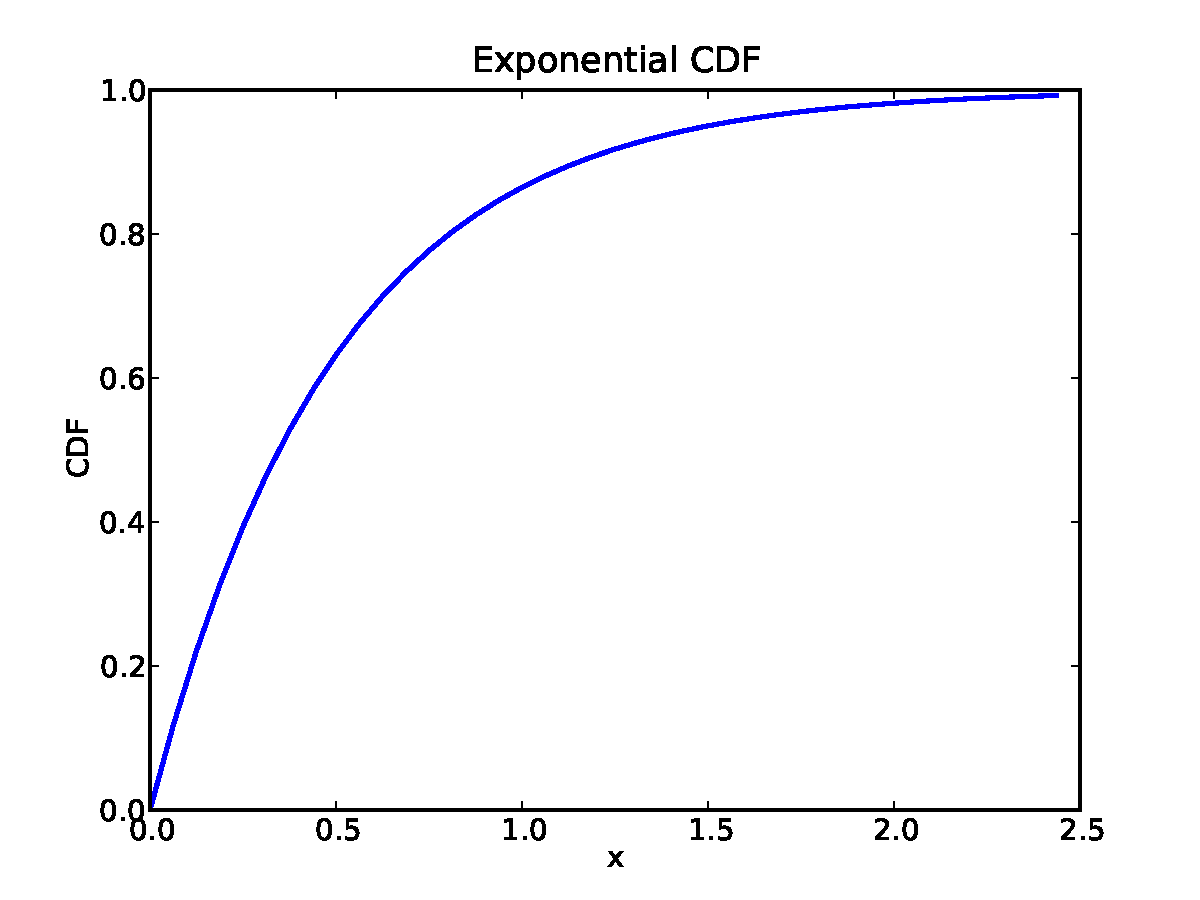
\includegraphics[height=2.5in]{figs/expo_cdf.pdf}}
\caption{CDF exponenciálního rozdělení.}
\label{expo_cdf}
\end{figure}

Obecně platí, že průměr exponenciálního rozdělení je 1\mydivide
\mylambda, takže průměr tohoto rozdělení je 0,5.  Medián je
ln(2)\mydivide\mylambda, což je zhruba 0,35.  \index{průměr}
\index{medián} \index{Austrálie} \index{Brisbane}

Jako příklad rozdělení, které je přibližně exponenciální, se podíváme na časový interval mezi jednotlivými narozeními.
18. prosince 1997 se v porodnici v Brisbane v Austrálii\footnote{Tento příklad vychází z informací a dat uvedených v Dunn, ``A Simple Dataset for Demonstrating Common Distributions,''
  Journal of Statistics Education v.7, n.3 (1999).} narodilo 44 dětí.  Časy narození všech 44 dětí byly zveřejněny v místních novinách. Data si můžete stáhnout z \url{http://thinkstats.com/babyboom.dat}.
\index{čas narození}

Obrázek~\ref{interarrival_cdf} ukazuje CDF časových intervalů mezi narozeními v minutách. Zdá se, že má obecný tvar exponenciálního rozdělení, ale jak toto rozdělení poznáme?
\index{komplementární CDF}
\index{CDF!komplementární}
\index{CCDF}

Jednou z možností je graficky znázornit komplementární CDF, 1~\minus~CDF(\x) pomocí logaritmické stupnice na ose \y.  Pro data z exponenciálního rozdělení je výsledkem přímka. Podívejme se na to, proč toto funguje.

Pokud graficky znázorníte komplementární CDF (CCDF) souboru dat, u kterého předpokládáte exponenciální charakter, pak očekáváte funkci jako:
%
\[ y \approx e^{-\lambda x} \]
%
Jestliže použijeme logaritmickou stupnici na obou stranách, dostaneme:

\Eqn{ log \y~\myapprox~-\mylambda \x }

Takže na logaritmické stupnici na ose \y~je CCDF přímka se sklonem
\minus\mylambda.
\index{logaritmická stupnice}
\index{komplementární CDF}
\index{CDF!komplementární}
\index{CCDF}

\begin{figure}
% babyboom.py
\centerline{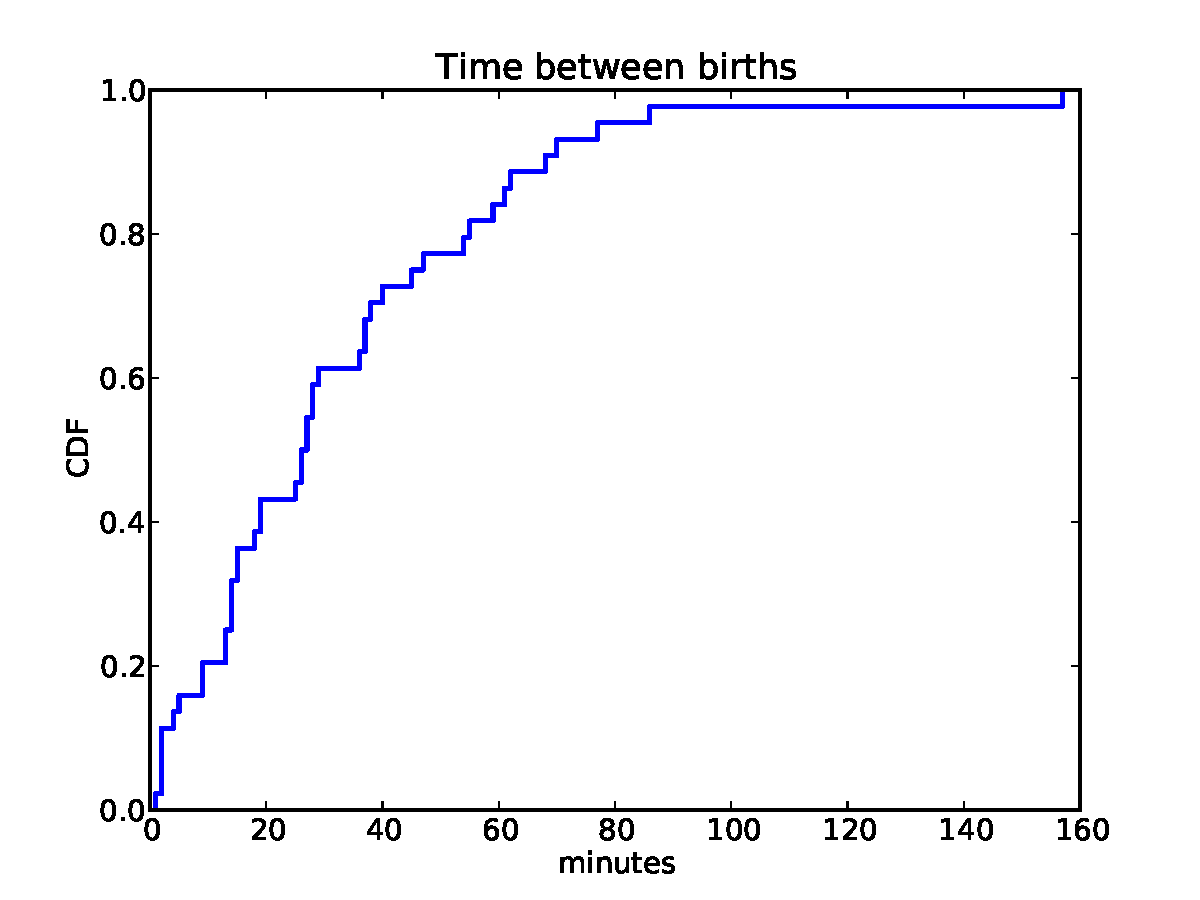
\includegraphics[height=2.5in]{figs/interarrivals.pdf}}
\caption{CDF časových intervalů mezi narozeními.}
\label{interarrival_cdf}
\end{figure}

\begin{figure}
% babyboom.py
\centerline{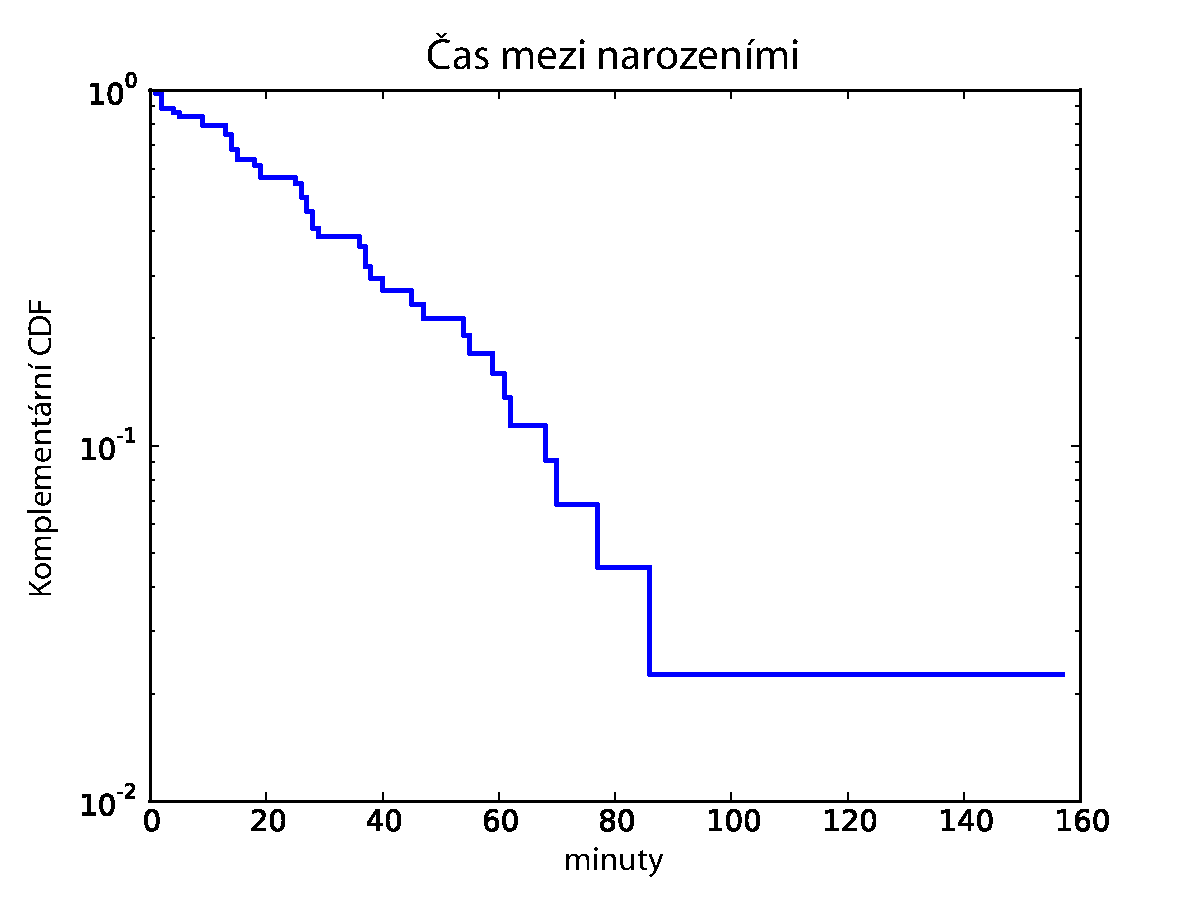
\includegraphics[height=2.5in]{figs/interarrivals_logy.pdf}}
\caption{CCDF časových intervalů mezi narozeními.}
\label{interarrival_ccdf}
\end{figure}

Obrázek~\ref{interarrival_ccdf} ukazuje CCDF časových intervalů mezi narozeními na logaritmické stupnici na ose
\y.  Nejedná se zcela o přímku, což naznačuje, že exponenciální rozdělení je pouhou aproximací.
Předpoklad, ze kterého vycházíme, -- že narození je stejně pravděpodobné v kterýkoliv okamžik dne -- neodpovídá s největší pravděpodobností zcela skutečnosti.

\begin{exercise}
U malých hodnot \n~neočekáváme, že se empirické rozdělení bude přesně shodovat se spojitým rozdělení. Jedním ze způsobů, jak vyhodnotit kvalitu souladu, je vytvořit výběr ze spojitého rozdělení a sledovat, jak dobře odpovídá datům.
\index{empirické rozdělení}
\index{rozdělení!empirické}
\index{modul random}

Funkce {\tt expovariate} v modulu {\tt random} generuje náhodné hodnoty z exponenciálního rozdělení se stanovenou hodnotou \mylambda.  Použijte ji k vygenerování 44 hodnot z exponenciálního rozdělení s průměrem 32,6. Graficky znázorněte CCDF na logaritmické stupnici na ose \y~a porovnejte ji s Obrázkem~\ref{interarrival_ccdf}.
\index{pyplot}

Nápověda: Ke grafickému znázornění pomocí logaritmické stupnice na ose \y~můžete použít funkci {\tt pyplot.yscale}.

% TODO: update this example

Nebo jestliže použijete {\tt myplot}, funkce {\tt Cdf} přijme booleovskou hodnotu parametru {\tt complement}, která určí, zda graficky znázorňovat CDF nebo CCDF, a řetězcové hodnoty parametrů {\tt xscale} a {\tt yscale}, které definují, jak budou osy vypadat. Pro grafické znázornění CCDF pomocí logaritmické stupnice na ose \y:
%
\begin{verbatim}
myplot.Cdf(cdf, complement=True, xscale='linear', yscale='log')
\end{verbatim}


\end{exercise}

\begin{exercise}
Shromážděte údaje o datech narození studentů ve vašem kurzu, setřiďte je a vypočítejte časový interval mezi daty narození ve dnech. Graficky znázorněte CDF časových intervalů mezi daty narození a CCDF na logaritmické stupnici na ose \y.  Vypadá to jako exponenciální rozdělení?
\index{exponenciální rozdělení}
\index{rozdělení!exponenciální}
\index{narozeniny}

\end{exercise}


\section{\protect\raggedright Paretovo rozdělení}
\index{Paretovo rozdělení}
\index{rozdělení!Paretovo}
\index{Pareto, Vilfredo}

Paretovo rozdělení je pojmenováno po ekonomovi Vilfredu Paretovi, který jej použil k popisu rozdělení bohatství (viz
\url{http://wikipedia.org/wiki/Pareto_distribution}).  Od té doby se používá k popisu jevů v přírodních i společenských vědách, včetně velikosti měst a obcí, částic prachu a meteoritů, lesních požárů a zemětřesení.
\index{CDF}

CDF Paretova rozdělení je následující:
%
\[ CDF(x) = 1 - \left( \frac{x}{x_m} \right) ^{-\alpha} \]
%
Parametry \x \sub{m} a \myalpha~určují umístění a tvar rozdělení. \x \sub{m} představuje minimální možnou hodnotu.
Obrázek~\ref{pareto_cdf} ukazuje CDF Paretova rozdělení s parametry \x \sub{m}~=~0,5 a \myalpha~=~1.
\index{parametr}

\begin{figure}
% continuous.py
\centerline{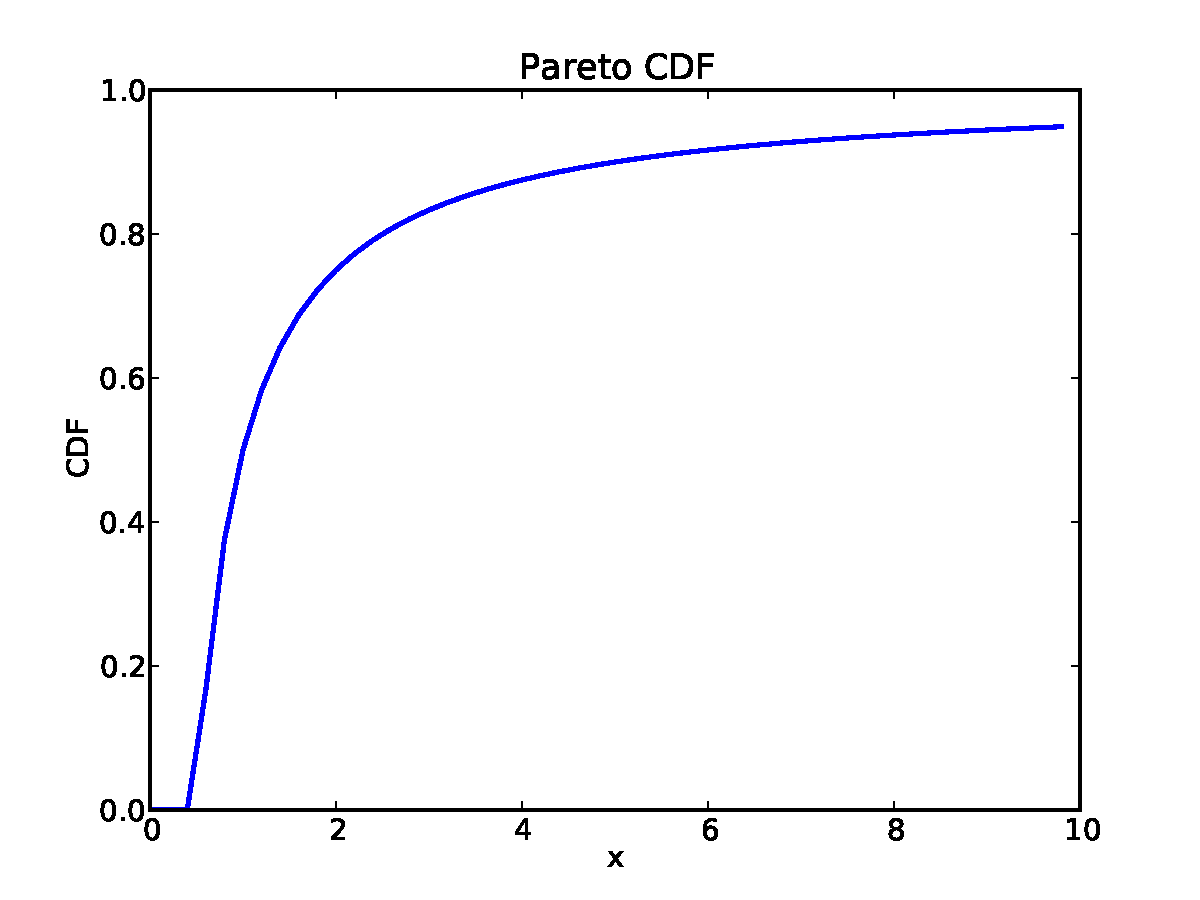
\includegraphics[height=2.5in]{figs/pareto_cdf.pdf}}
\caption{CDF Paretova rozdělení.}
\label{pareto_cdf}
\end{figure}

Medián tohoto rozdělení je $x_m 2^{1/\alpha}$, tedy 1, ale
 95. percentil je 10.  Naproti tomu v případě exponenciálního rozdělení s mediánem 1 má 95. percentil hodnotu pouze 1,5.  \index{exponenciální rozdělení} \index{rozdělení!exponenciální} \index{medián}
\index{logaritmická stupnice}

Existuje jednoduchý vizuální test k určení toho, zda se empirické rozdělení shoduje s Paretovým rozdělením: Pokud pro obě osy použijeme logaritmickou stupnici, CCDF má podobu přímky. Jestliže graficky znázorníte CCDF výběru z Paretova rozdělení na lineární stupnici, očekáváte funkci, která bude vypadat takto:
%
\[ y \approx \left( \frac{x}{x_m} \right) ^{-\alpha} \]
%
Když použijeme logaritmickou stupnici na obou stranách, získáme:

\Eqn{ log y \myapprox \minus\myalpha~(log \x~\minus~log x\sub{m}) }

Jestliže tedy provedete grafické znázornění log \y~versus log \x, výsledkem by měla být přímka se sklonem \minus\myalpha~a konstantou \myalpha~log \x\sub{m}.

\begin{exercise}
Modul {\tt random} nabízí funkci {\tt paretovariate},
která generuje náhodné hodnoty z Paretova rozdělení.  Přijme parametr pro
\myalpha, ale nikoliv \x\sub{m}. Implicitní hodnota
\x\sub{m} je 1; rozdělení s jiným parametrem můžete vygenerovat vynásobením hodnotou \x\sub{m}.
\index{modul random}
\index{Paretovo rozdělení}
\index{rozdělení!Paretovo}

Napište wrapper funkci s názvem {\tt paretovariate}, která přijme
\myalpha~a \x \sub{m} jako parametry použije {\tt
  random.paretovariate} k vygenerování hodnot z dvouparametrického Paretova rozdělení.
\index{parametr}

Použijte svoji funkci k vygenerování výběru z Paretova rozdělení. Vypočtěte
CCDF a graficky ji znázorněte pomocí logaritmické stupnice na obou osách. Je výsledkem přímka? Jaký je sklon?
\index{komplementární CDF}
\index{CDF!komplementární}
\index{CCDF}

\end{exercise}

\begin{exercise}
Abyste získali určitý cit pro Paretova rozdělení, představte si, jak by vypadal svět, pokud by rozdělení výšek lidí mělo podobu Paretova rozdělení. Na základě parametrů \x \sub{m}~=~100 cm a \myalpha~=~1,7 získáme rozdělení s přiměřeným minimem 100 cm a mediánem 150 cm.
\index{výška}

Vygenerujte 6 miliard náhodných hodnot z tohoto rozdělení. Jaký je průměr tohoto vzorku?  Jaká část populace je nižší než průměr? Jakou výšku má nejvyšší člověk ve světě, kterému vládne Paretovo rozdělení?
\index{svět Paretova rozdělení}

\end{exercise}

\begin{exercise}
Zipfův zákon je založen na pozorování četnosti užití různých slov. Nejběžnější slova mají velmi vysokou četnost. Na druhé straně existuje řada neobvyklých slov, jako například ``hapax legomenon'', která se vyskytují jen několikrát. Zipfův zákon předpokládá, že v určitém souboru textů označovaném jako ``korpus'' bude rozdělení četnosti výskytu slov zhruba odpovídat Paretovu rozdělení.
\index{Paretovo rozdělení}
\index{rozdělení!Paretovo}
\index{Zipfův zákon}
\index{hapax legomenon}
\index{korpus}
\index{četnost}
\index{četnost slova}

Najděte velký korpus pro jakýkoliv jazyk, který je dostupný v elektronické podobě. Spočítejte, kolikrát se v něm vyskytují jednotlivá slova. Zjistěte CCDF četnosti výskytu slov a graficky ji znázorněte pomocí logaritmické stupnice na obou osách. Platí Zipfův zákon? Jaká je, přibližně, hodnota \myalpha?
\index{komplementární CDF}
\index{CDF!komplementární}
\index{CCDF}

\end{exercise}

\begin{exercise}
\label{weibull}


Weibullovo rozdělení je zobecněním exponenciálního rozdělení, které se vyskytuje v analýze poruch
(viz \url{http://wikipedia.org/wiki/Weibull_distribution}).  CDF tohoto rozdělení je:
%
\[ CDF(x) = 1 - e^{-(x / \lambda)^k} \]
%
Najdete transformaci, jejíž pomocí získá Weibullovo rozdělení podobu přímky? Co naznačují směrnice a konstantní člen/konstanta přímky?
\index{Weibullovo rozdělení}
\index{rozdělení!Weibullovo}
\index{exponenciální rozdělení}
\index{rozdělení!exponenciální}
\index{modul random}

Použijte {\tt random.weibullvariate} k vygenerování výběru z Weibullova rozdělení a použijte jej k otestování vaší transformace.

\end{exercise}


\section{\protect\raggedright Normální rozdělení}
\label{normal}
\index{normální rozdělení}
\index{rozdělení!normální}
\index{Gaussovo rozdělení}
\index{rozdělení!Gaussovo}

\newcommand{\erf}{\mathrm{erf}}

Normální rozdělení, nazývané také Gaussovo, se používá nejčastěji, protože jeho prostřednictvím lze popsat velké množství jevů, tedy alespoň přibližně. Ukazuje se, že pro jeho všudypřítomnost existuje velmi dobrý důvod, k němuž se dostaneme v Oddílu
~\ref{CLT}.
\index{chybová funkce}
\index{CDF}

Normální rozdělení se vyznačuje řadou vlastností, které jej činí vhodným pro analýzu, ale CDF k nim nepatří.
Na rozdíl od ostatních rozdělení, jimiž jsme se zde zabývali, pro normální distribuční funkci neexistuje žádné vyjádření s uzavřenou formou; nejčastěji využívanou alternativou je její zápis prostřednictvím
 {\bf chybové funkce}, což je speciální funkce zapsaná jako erf(\x):
%
\[ CDF(x) = \frac{1}{2} \left[ 1 +
  \erf \left( \frac{x - \mu}{\sigma \sqrt{2}} \right) \right] \]
%
\[ \erf(x) = \frac{2}{\sqrt{\pi}} \int_{0}^x e^{-t^2} dt \]
%
Parametry \mymu~a \mysigma~určují průměr a směrodatnou odchylku rozdělení.
\index{parametr}
\index{{\tt erf.py}}

Jestli vás z těchto vzorců bolí oči, nezoufejte, protože je snadné je provést v Pythonu\footnote{Od verze Python 3.2 je to dokonce ještě snazší, protože {\tt erf} je obsažena v modulu {\tt math}.}.  Existuje celá řada rychlých a přesných způsobů, jak přiblížit erf(\x).  Jeden z nich si můžete stáhnout na \url{http://thinkstats.com/erf.py}, kde najdete funkce nazvané
{\tt erf} a {\tt NormalCdf}.

Obrázek~\ref{normal_cdf} ukazuje CDF normálního rozdělení s parametry \mymu~=~2,0 a \mysigma~=~0,5.  Signoidní tvar křivky je znakem, podle něhož je možné poznat normální rozdělení.

\begin{figure}
% continuous.py
\centerline{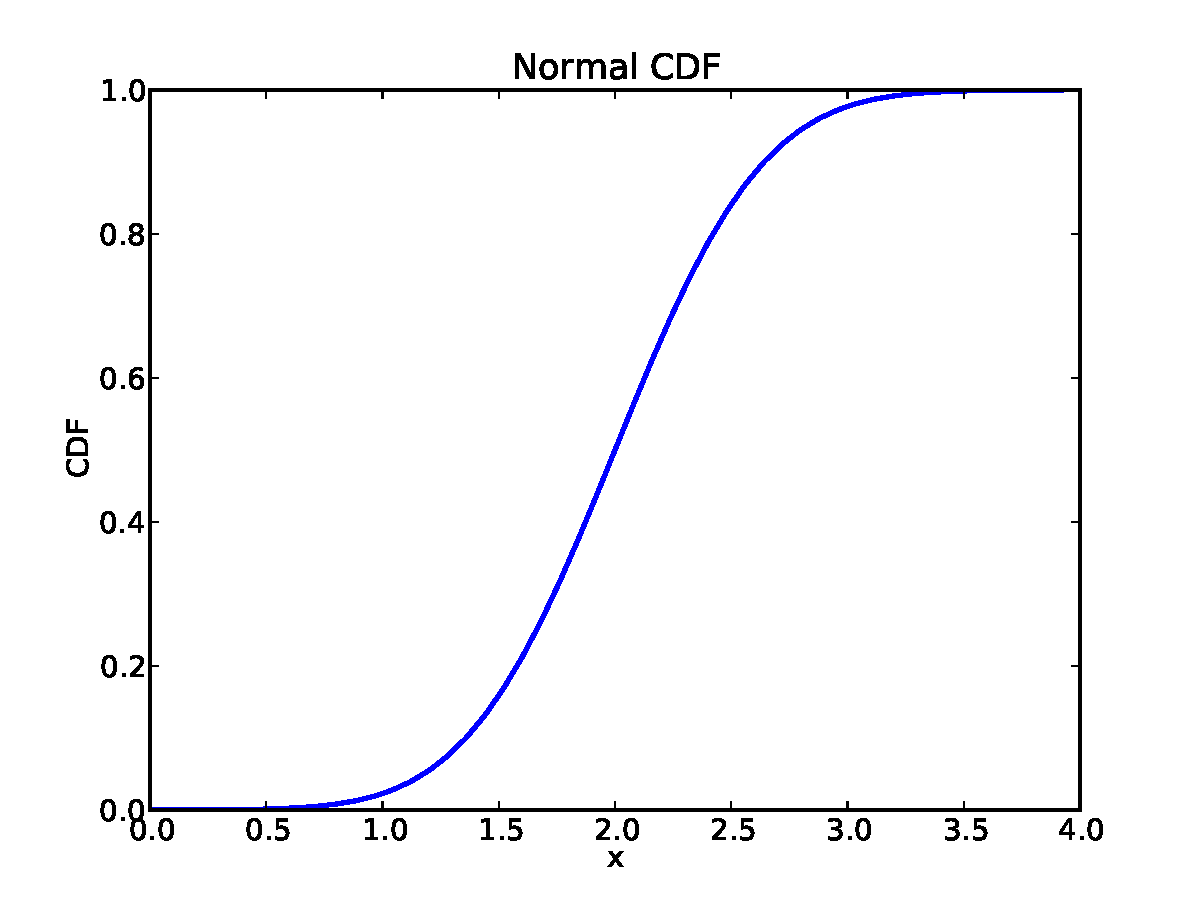
\includegraphics[height=2.5in]{figs/normal_cdf.pdf}}
\caption{CDF normálního rozdělení.}
\label{normal_cdf}
\end{figure}

V předchozí kapitole jsme se zabývali rozdělením porodních hmotností v souboru dat NSFG.
Obrázek~\ref{nsfg_birthwgt_model} ukazuje empirickou
CDF hmotností všech živě narozených dětí a CDF normálního rozdělení se stejným průměrem a rozptylem.
\index{Národní šetření růstu rodin -- National Survey of Family Growth}
\index{NSFG}
\index{porodní hmotnost}
\index{hmotnost!porodní}

\begin{figure}
% continuous.py
\centerline{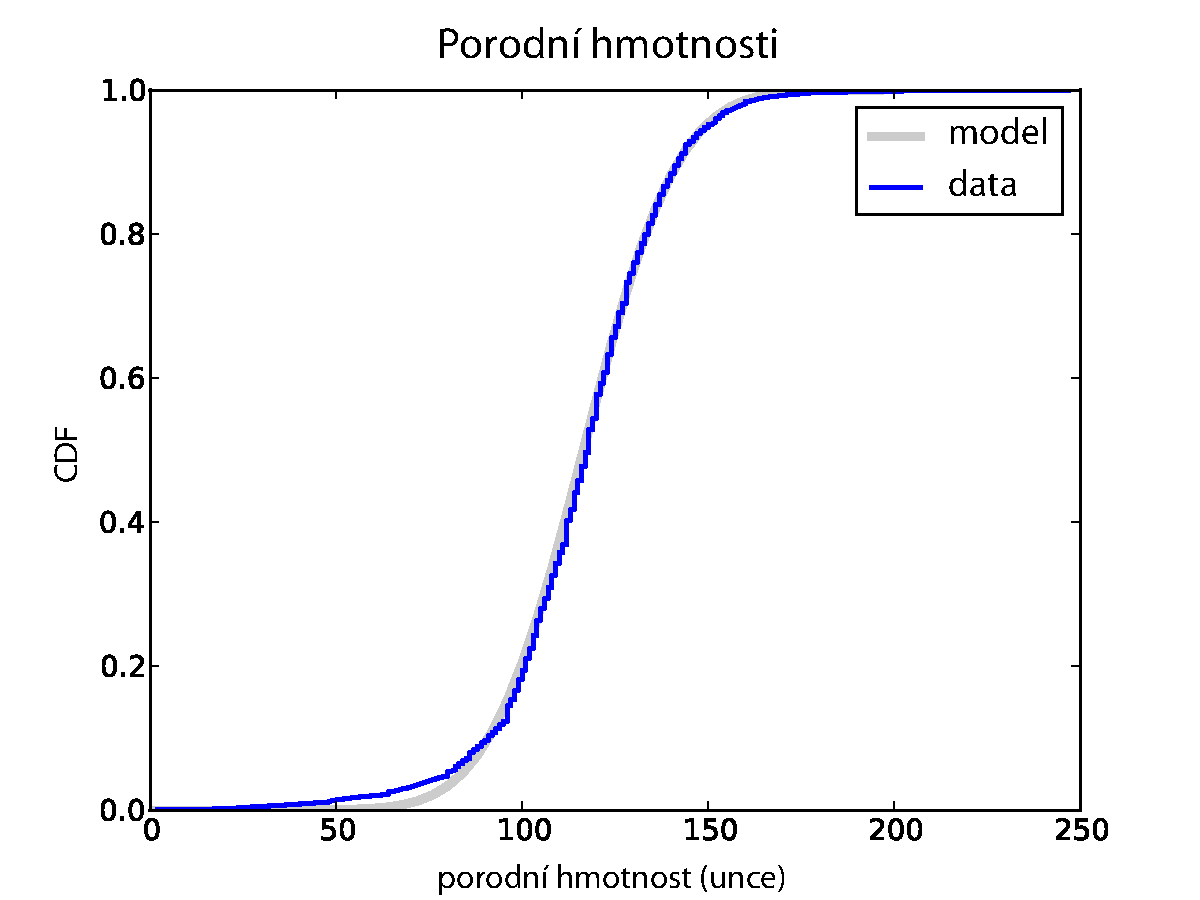
\includegraphics[height=2.5in]{figs/nsfg_birthwgt_model.pdf}}
\caption{CDF porodních hmotností s normálním modelem.}
\label{nsfg_birthwgt_model}
\end{figure}

Normální rozdělení je dobrým modelem pro tento soubor dat.  {\bf
 Model} představuje užitečné zjednodušení.  V tomto případě je užitečný, protože celé rozdělení můžeme shrnout pomocí pouhých dvou čísel \mymu~=~116,5 a \mysigma~=~19,9, přičemž výsledná chyba
(rozdíl mezi modelem a daty) je malá.
\index{model}
\index{percentil}

Pod 10. percentilem dochází k rozporu mezi daty a modelem; je zde více dětí s nízkou hmotností, než bychom očekávali v normálním rozdělení. Pokud chceme studovat předčasně narozené děti, je důležité zachytit tuto část rozdělení správně. Z tohoto důvodu by normální model nemusel být vhodný.

\begin{exercise}
Wechslerova škála inteligence dospělých je test, který je určen k měření inteligence\footnote{Kolem otázky, zda ji opravdu měří či neměří, se vedou fascinující spory, jejichž zkoumání stojí za to věnovat svůj čas.}.  Výsledky jsou transformovány tak, že rozdělení skóre v obecné populaci je normální s \mymu~=~100 a \mysigma~=~15.
\index{Wechslerova škála inteligence dospělých}
\index{škála inteligence dospělých}
\index{WAIS}
\index{IQ}
\index{inteligence}

Použijte {\tt erf.NormalCdf} k prozkoumání četnosti jevů, které se v normálním rozdělení vyskytují řídce. Jaká část populace
má IQ vyšší než průměr? Jaká část má IQ nad 115?  130?  145?

Jev, který můžeme označit jako ``six sigma'', je hodnota přesahující průměr o 6 směrodatných odchylek, takže six sigma IQ je 190.  Kolik předpokládáte, že na světě se 6 miliardami lidí žije jedinců s IQ 190 nebo vyšším\footnote{V souvislosti s tímto tématem by vás mohlo zajímat toto:  \url{http://wikipedia.org/wiki/Christopher_Langan}.}?
\index{Langan, Christopher}
\index{jev!six sigma}

\end{exercise}


\begin{exercise}
Graficky znázorněte CDF délek těhotenství pro všechny živě narozené děti. Má výsledek podobu normálního rozdělení?
\index{délka těhotenství}

Vypočtěte průměr a směrodatnou odchylku výběru a graficky znázorněte normální rozdělení se stejnými parametry. Představuje normální rozdělení dobrý model pro tato data? Pokud byste měli shrnout toto rozdělení dvěma statistickými charakteristikami, které byste zvolili?

\end{exercise}


\section{\protect\raggedright Normální pravděpodobnostní graf}
\index{normální pravděpodobnostní graf}
\index{graf!normální pravděpodobnostní}
\index{exponenciální rozdělení}
\index{rozdělení!exponenciální}
\index{Weibullovo rozdělení}
\index{rozdělení!Weibullovo}
\index{Paretovo rozdělení}
\index{rozdělení!Paretovo}

Pro exponenciální, Paretovo a Weibullovo rozdělení existují jednoduché transformace, které můžeme použít, chceme-li otestovat, jestli spojité rozdělení představuje vhodný model pro konkrétní soubor dat.
\index{model}
\index{normální rozdělení}
\index{rozdělení!normální}
\index{Gaussovo rozdělení}
\index{rozdělení!Gaussovo}

Pro normální rozdělení žádná takováto transformace k dispozici není, ale
existuje alternativní možnost označovaná jako {\bf normální pravděpodobnostní graf}. Ten je založen na
{\bf rankits}: jestliže vygenerujete \n~hodnot z normálního rozdělení a setřídíte je, pak \kk-tý rankit je průměr rozdělení pro
\kk-tou hodnotu.
\index{rankit}

\begin{exercise}
Napište funkci s názvem {\tt Sample}, která vygeneruje 6 vzorků z normálního rozdělení, kde
\mymu~=~0 a \mysigma~=~1.  Setřiďte a vraťte hodnoty.

Napište funkci s názvem {\tt Samples}, která volá {\tt Sample} 1000x a vrátí seznam 1000 seznamů.

Jestliže na tento seznam seznamů aplikujete funkci {\tt zip}, výsledkem bude 6 seznamů, každý o 1000 hodnotách. Vypočtěte průměr každého z těchto seznamů a vytiskněte výsledky. Můj odhad je, že vám vyjde něco jako:

\{\minus1,2672,   \minus0,6418,   \minus0,2016,   0,2016,   0,6418,   1,2672\}

Pokud zvýšíte počet volání funkce {\tt Sample}, výsledky by měly konvergovat k těmto hodnotám.

\end{exercise}

% Algorithms for exact and approximate normal rank stats
% http://download.osgeo.org/grass/grass6_progman/as177_8c_source.html

Přesně vypočíst rankits je mírně obtížné, ale existují numerické metody, jak je přiblížit. A existuje také rychlá a hrubá metoda, kterou je ještě jednodušší použít:
\begin{enumerate}

\item Z normální distribuce, kde \mymu~=~0 a \mysigma~=~1,
vytvořte výběr o stejném rozsahu jako váš soubor dat a setřiďte jej.

\item Setřiďte hodnoty v souboru dat.

\item Graficky znázorněte setříděné hodnoty z vašeho souboru dat versus náhodné hodnoty.

\end{enumerate}

Tato metoda funguje dobře pro velké soubory dat. Pro menší soubory dat je možné ji vylepšit vygenerováním
\m (\n+1)~\minus~1 hodnot z normálního rozdělení, kde \n~ je rozsah souboru dat a
\m~je multiplikátor.  Pak vyberte každý \m-tý prvek, počínaje \m-tým.

%Hint: use the Python slice operator.

Tato metoda funguje také pro další rozdělení za předpokladu, že víte, jak vygenerovat náhodný výběr.

Obrázek~\ref{nsfg_birthwgt_normal} představuje rychlý a hrubý normální pravděpodobnostní graf pro data porodních hmotností.
\index{porodní hmotnost}
\index{hmotnost!porodní}

\begin{figure}
% continuous.py
\centerline{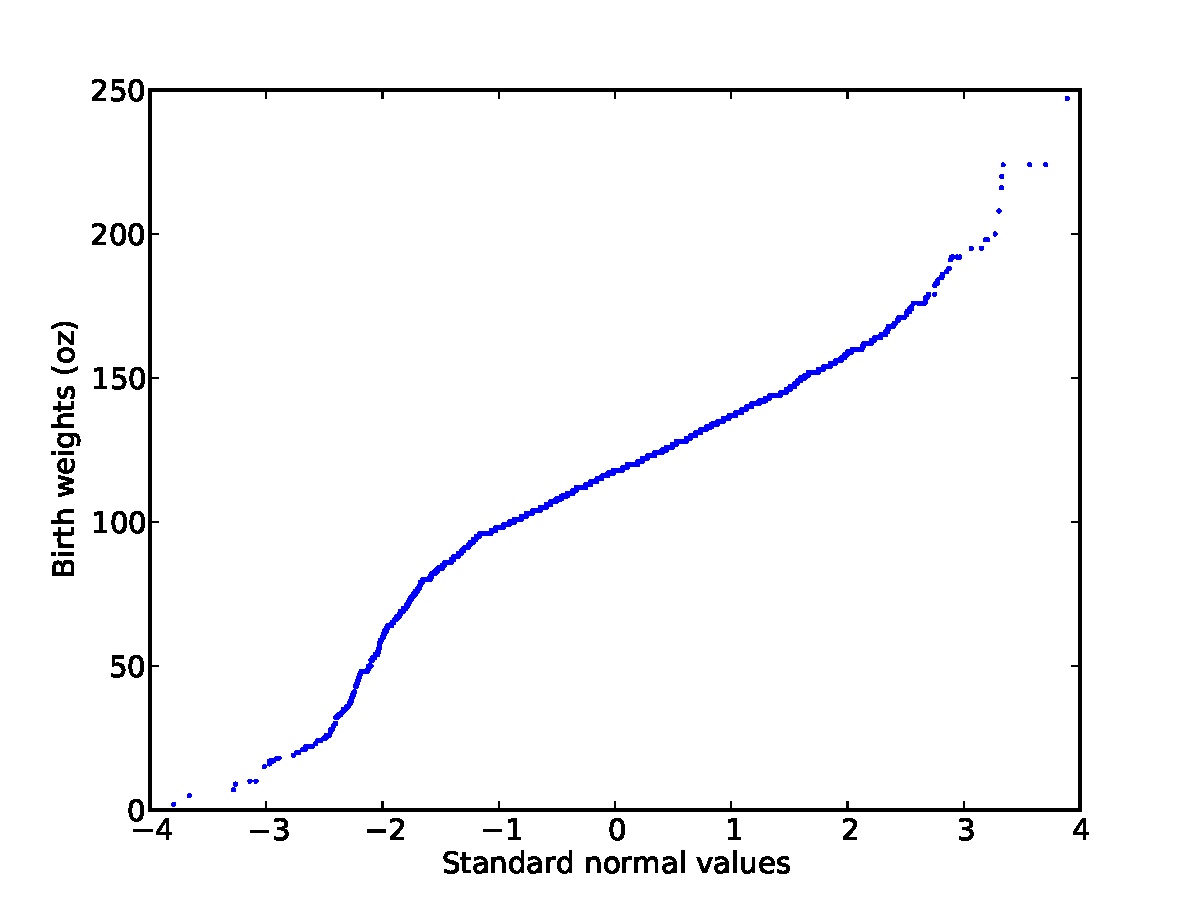
\includegraphics[height=2.5in]{figs/nsfg_birthwgt_normal.pdf}}
\caption{Normální pravděpodobnostní graf porodních hmotností.}
\label{nsfg_birthwgt_normal}
\end{figure}

Zakřivení tohoto grafu naznačuje určité odchylky od normálního rozdělení, ale přesto se jedná o (dostatečně) dobrý model pro celou řadu účelů.
\index{model}

\begin{exercise}
Napište funkci s názvem {\tt NormalPlot}, která přijme řadu hodnot a vygeneruje normální pravděpodobnostní graf. Řešení si můžete stáhnout z \url{http://thinkstats.com/rankit.py}.
\index{normální rozdělení}
\index{rozdělení!normální}
\index{Gaussovo rozdělení}
\index{rozdělení!Gaussovo}
\index{{\tt rankit.py}}
\index{{\tt relay.py}}
\index{{\tt relay\_normal.py}}
\index{štafetový závod}
\index{závod!štafetový}

Použijte běžecké rychlosti z {\tt relay.py} k vygenerování normálního pravděpodobnostního grafu.
Je normální rozdělení dobrým modelem pro tato data? Řešení si můžete stáhnout z
\url{http://thinkstats.com/relay_normal.py}.

\end{exercise}


\section{\protect\raggedright Logaritmicko-normální rozdělení}
\label{lognormal}
\index{logaritmicko-normální rozdělení}
\index{rozdělení!logaritmicko-normální}
\index{CDF}

Jestliže logaritmy množiny hodnot vykazují normální rozdělení, tyto hodnoty mají {\bf logaritmicko-normální} (také {\bf lognormální}) rozdělení.
CDF logaritmicko-normálního rozdělení je stejné jako CDF normálního rozdělení, kde \x~je nahrazeno log \x.

\Eqn{ CDF\sub{lognormal}(\x) = CDF\sub{normal}(log \x) }

Parametry logaritmicko-normálního rozdělení se obvykle označují jako \mymu~a \mysigma.  Nezapomeňte ale, že tyto parametry {\em nejsou} průměr a směrodatná odchylka. Průměr logaritmicko-normálního rozdělení je exp(\mymu~+~\sigmasq/2) a směrodatná odchylka je nepěkná\footnote{Viz \url{http://wikipedia.org/wiki/Log-normal_distribution}.}.
\index{parametr} \index{hmotnost!dospělých} \index{hmotnost dospělých}

Ukazuje se, že rozdělení hmotností dospělých je přibližně logaritmicko-normální
\footnote{Na tuto možnost mě upozornil komentář (bez citace) na
 \url{http://mathworld.wolfram.com/LogNormalDistribution.html}.
  Následně jsem našel článek, ve kterém je navržena logaritmická transformace a také je zde naznačena příčina:
 Penman and Johnson, ``The Changing Shape of the
  Body Mass Index Distribution Curve in the Population,'' Preventing
  Chronic Disease, 2006 July; 3(3): A74.  Online
  at \url{http://www.ncbi.nlm.nih.gov/pmc/articles/PMC1636707}.}.

Národní centrum pro prevenci chronických onemocnění a podporu zdraví (National Center for Chronic Disease
Prevention and Health Promotion) provádí každoroční šetření jako součást Systému sledování rizikových faktorů chování (Behavioral Risk Factor Surveillance System --
BRFSS)\footnote{Centers for Disease Control and Prevention
  (CDC). Behavioral Risk Factor Surveillance System Survey
  Data. Atlanta, Georgia: U.S. Department of Health and Human
  Services, Centers for Disease Control and Prevention, 2008.}.  V roce
2008 se do šetření zapojilo 414 509 respondentů, kteří byli dotázáni na jejich demografické údaje, zdraví a zdravotní rizika.
\index{Systém sledování rizikových faktorů chování -- Behavioral Risk Factor Surveillance System}
\index{BRFSS}


\begin{figure}
% cumulative.py
\centerline{
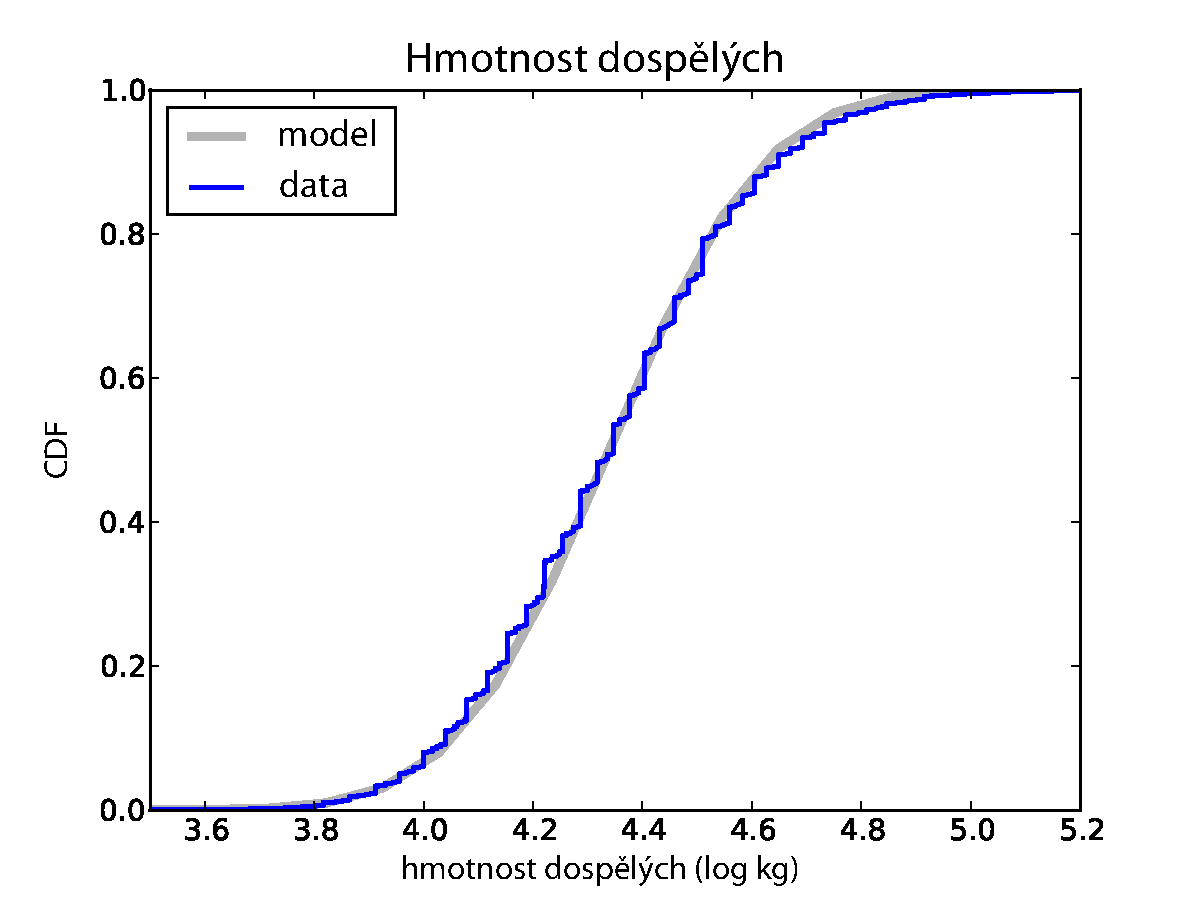
\includegraphics[height=2.5in]{figs/brfss_weight_log.pdf}
}
\caption{CDF hmotností dospělých (logaritmická transformace).}
\label{brfss_weight_log}
\end{figure}

Shromážděná data zahrnují hmotnosti 398 484 respondentů vyjádřené v kilogramech.
Obrázek~\ref{brfss_weight_log} ukazuje rozdělení log \w, kde \w~je hmotnost v kilogramech, spolu s normálním modelem.
\index{respondent}
\index{model}

Normální model vyjadřuje dobrou shodu s daty, přestože nejvyšší hmotnosti přesahují to, co bychom očekávali od normálního modelu dokonce i po provedení logaritmické transformace.  Protože rozdělení log \w~odpovídá normálnímu rozdělení, vede nás to k závěru, že \w~odpovídá logaritmicko-normálnímu rozdělení.
\index{normální rozdělení}
\index{rozdělení!normální}
\index{Gaussovo rozdělení}
\index{rozdělení!Gaussovo}
\index{logaritmicko-normální rozdělení}
\index{rozdělení!logaritmicko-normální}


%Figure~\ref{brfss_weight_model} shows the
%distribution of these weights and a normal model with the same mean
%and variance.

%\begin{figure}
%\centerline{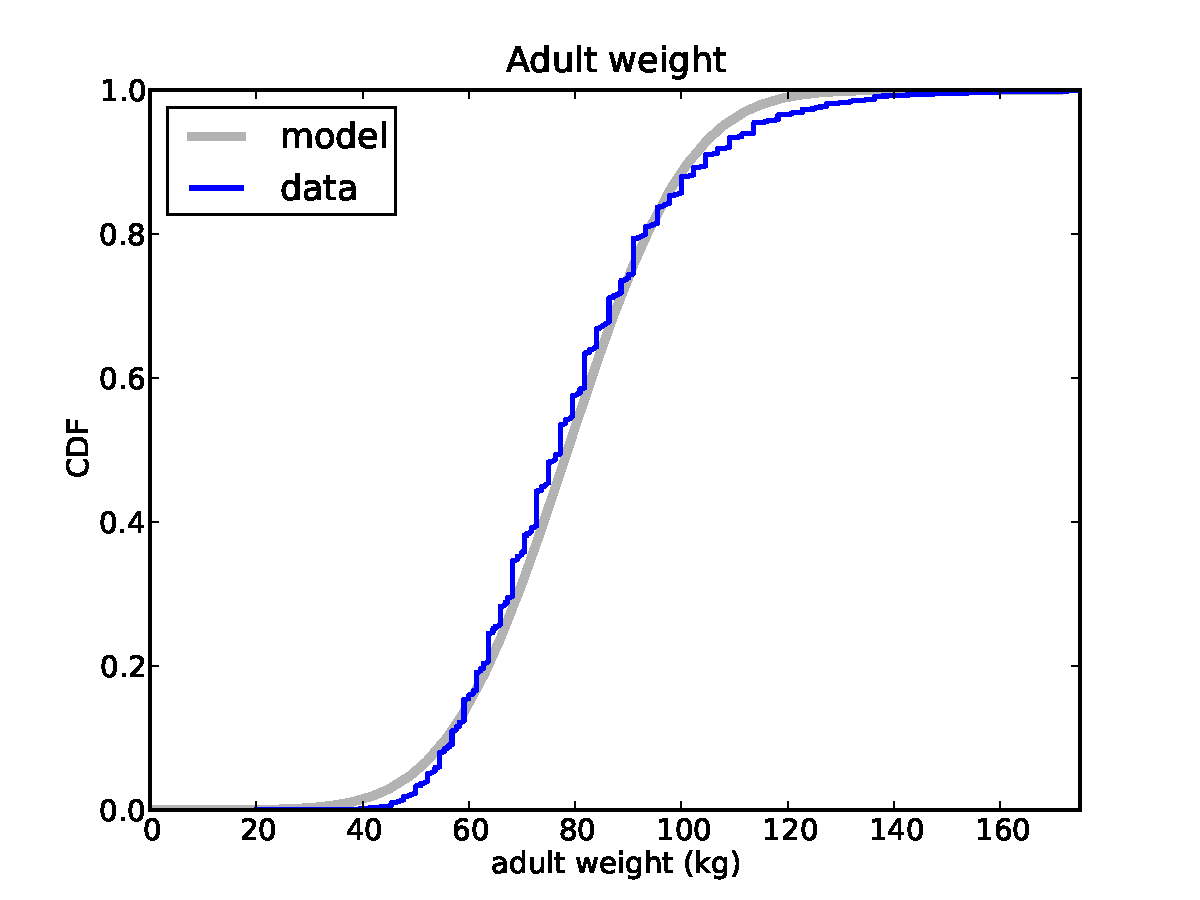
\includegraphics[height=2.5in]{figs/brfss_weight_model.pdf}}
%\caption{CDF of adult weights from the BRFSS.}
%\label{brfss_weight_model}
%\end{figure}

%The agreement between the data and the model might be good enough
%for some purposes, but there are clear discrepancies below the 10th
%and above the 90th percentile.

%\begin{figure}
%\centerline{
%\begin{tabular}{cc}
%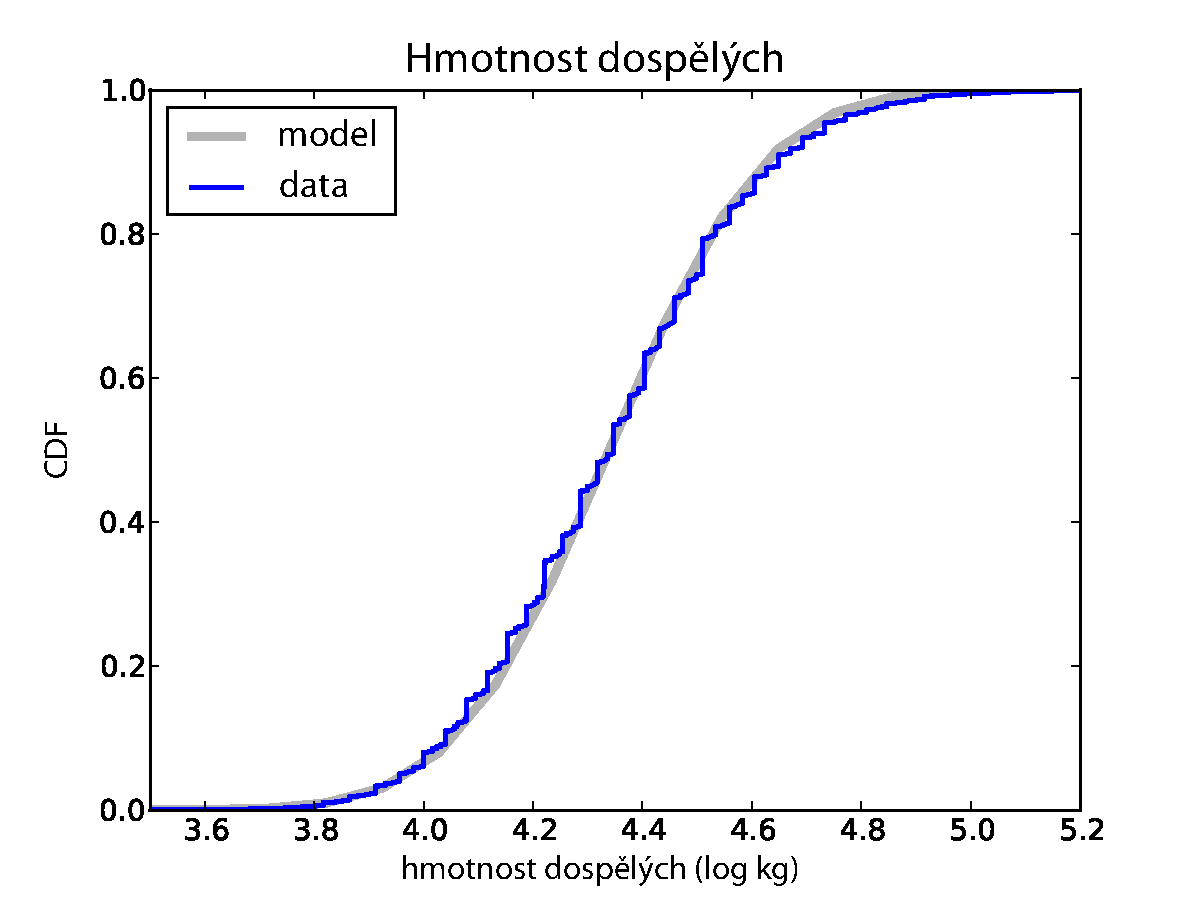
\includegraphics[height=2.3in]{figs/brfss_weight_log.pdf}
%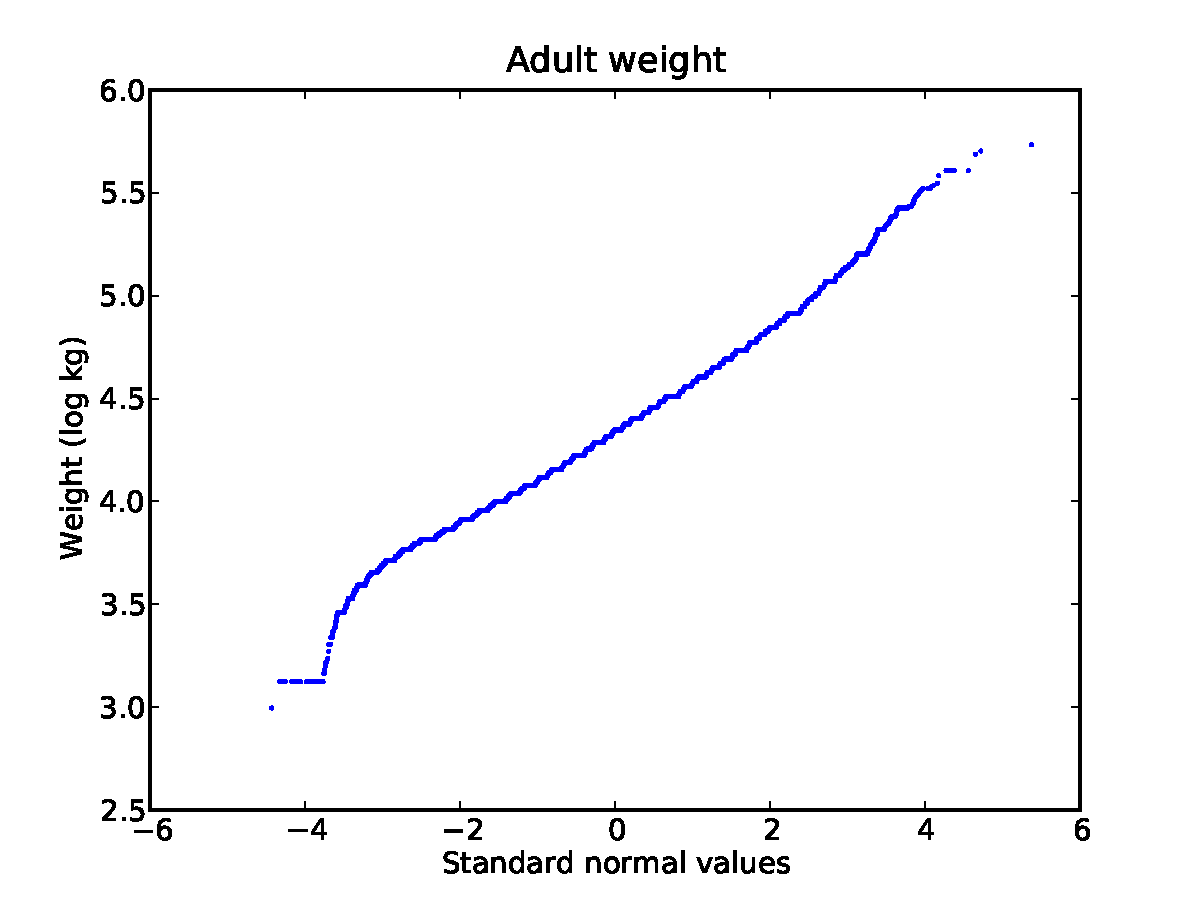
\includegraphics[height=2.3in]{figs/brfss_weight_lognormal.pdf}
%\end{tabular}
%}
%\caption{CDF and normal probability plot for adult weights (log
%  transform).}
%\label{brfss_weight_log}
%\end{figure}

\begin{exercise}
Stáhněte si data z BRFSS na
\url{http://thinkstats.com/CDBRFS08.ASC.gz} a můj kód vytvořený k jejich přečtení na
\url{http://thinkstats.com/brfss.py}.  Spusťte {\tt brfss.py} a potvrďte tisk souhrnných statistických charakteristik pro několik proměnných.
\index{Systém sledování rizikových faktorů chování -- Behavioral Risk Factor Surveillance System}
\index{BRFSS}
\index{{\tt brfss.py}}
\index{{\tt brfss\_figs.py}}
\index{hmotnost!dospělých}
\index{hmotnost dospělých}

Napište program, který přečte hmotnosti dospělých z BRFSS a vygeneruje normální pravděpodobnostní grafy pro
\w~a log \w.  Řešení si můžete stáhnout z
\url{http://thinkstats.com/brfss_figs.py}.

\end{exercise}

\begin{exercise}
Rozdělení počtu obyvatel pro města a obce bylo uvedeno jako příklad jevu z reálného světa, který lze popsat pomocí Paretova rozdělení.
\index{Paretovo rozdělení}
\index{rozdělení!Paretovo}
\index{Americký úřad pro sčítání lidu -- U.S.~Census Bureau}
\index{populace}
\index{velikost města}

Americký úřad pro sčítání lidu (U.S.~Census Bureau) zveřejňuje údaje o počtu obyvatel každého města a obce ve Spojených státech, které má vlastní samosprávu. Vytvořil jsem malý program, který si stáhne tato data a uloží je do souboru. Můžete si jej stáhnout na
 \url{http://thinkstats.com/populations.py}.
\index{{\tt populations.py}}

\begin{enumerate}

\item Pročtěte si tento program, ať víte, co umí. Pak jej spusťte, abyste stáhli a zpracovali data.

\item Napište program, který spočítá a graficky znázorní rozdělení počtu obyvatel 14 593 měst a obcí v souboru dat.

\item Graficky znázorněte CDF na lineární stupnici a logaritmické stupnici na ose \x, tak abyste získali představu o tvaru tohoto rozdělení. Pak graficky znázorněte CCDF na logaritmické stupnici pro obě osy, abyste zjistili, jestli má tvar charakteristický pro Paretovo rozdělení.
\index{komplementární CDF}
\index{CDF!komplementární}
\index{CCDF}

\item Vyzkoušejte ostatní transformace a grafy v této kapitole, abyste zjistili, jestli pro tato data existuje lepší model.

\end{enumerate}

K jakému závěru jste dospěli ohledně rozdělení velikosti měst a obcí? Řešení si můžete stáhnout z
\url{http://thinkstats.com/populations_cdf.py}.
\index{{\tt populations\_cdf.py}}

\end{exercise}


\begin{exercise}
\label{irs}

Daňová správa USA (The Internal Revenue Service of the United States  -- IRS) uvádí data o daních z příjmů na
\url{http://irs.gov/taxstats}.
\index{Daňová správa USA -- Internal Revenue Service}
\index{IRS}
\index{příjem}
\index{daně}

Jeden ze souborů tohoto úřadu obsahující údaje o příjmech fyzických osob za rok 2008 je dostupný na \url{http://thinkstats.com/08in11si.csv}.  Převedl jsem jej do textového formátu označovaného zkratkou CSV, což znamená
``hodnoty oddělené čárkou'' (comma-separated values). Můžete si jej přečíst pomocí modulu {\tt csv}.

Extrahujte rozdělení příjmů z tohoto souboru dat. Představuje některé ze spojitých rozdělení uvedených v této kapitole dobrý model pro tato data? Řešení si můžete stáhnout z \url{http://thinkstats.com/irs.py}.
\index{{\tt irs.py}}

\end{exercise}


\section{\protect\raggedright Proč model?}
\index{model}

Na začátku této kapitoly jsem řekl, že spojitá rozdělení lze použít k modelování mnoha jevů reálného světa.
``Takže,'' mohli byste se zeptat, ``kterých?''
\index{abstrakce}

Stejně jako všechny modely, jsou také spojitá rozdělení abstrakcí, což znamená, že vynechávají určité detaily, jež nejsou považovány za důležité. Například pozorované rozdělení může obsahovat chyby měření nebo zvláštnosti specifické pro daný výběr. Spojité modely přitom tyto idiosynkrazie vyhlazují.
\index{vyrovnání}

Spojité modely jsou zároveň formou komprese dat. Jestliže nějaký model dobře přiléhá k souboru dat, pak je možné pomocí malé množiny parametrů souhrnně popsat velký objem dat.
\index{parametr}
\index{komprese}

Někdy může být skutečnost, že data týkající se určitého přírodního jevu odpovídají spojitému rozdělení, překvapivá, avšak takováto pozorování mohou vést k novým vhledům do fyzických systémů. Někdy jsme schopni vysvětlit, proč pozorované rozdělení má určitou formu. Například Paretovo rozdělení je často výsledkem generativních procesů s kladnou zpětnou vazbou (tzv. procesů preferenčního připojování (preferential attachment processes): viz
\url{http://wikipedia.org/wiki/Preferential_attachment}.).
\index{preferenční připojování}
\index{generativní proces}
\index{Paretovo rozdělení}
\index{rozdělení!Paretovo}
\index{analýza}

Spojitá rozdělení jsou vhodná pro matematickou analýzu, jak si ukážeme v Kapitole~\ref{operations}.


\section{\protect\raggedright Generování náhodných čísel}
\index{exponenciální rozdělení}
\index{rozdělení!exponenciální}
\index{náhodné číslo}
\index{CDF}
\index{algoritmus inverzní CDF}
\index{rovnoměrné rozdělení}
\index{rozdělení!rovnoměrné}

Spojité CDFs jsou také vhodné pro generování náhodných čísel.
Jestliže existuje efektivní způsob, jak vypočíst inverzní CDF, ICDF(\p),
můžeme vygenerovat náhodné hodnoty s vhodným rozdělením na základě výběru z rovnoměrného rozdělení od
0 do 1, a následnou volbou

\Eqn{ \x~=~ICDF(\p) }

Například CDF exponenciálního rozdělení je
%
\[ p = 1 - e^{-\lambda x} \]
%
Řešením pro \x~získáme:

\Eqn{ \x = \minus log (1~\minus~\p) / \mylambda }

V Pythonu tedy můžeme napsat
%
\begin{verbatim}
def expovariate(lam):
    p = random.random()
    x = -math.log(1-p) / lam
    return x
\end{verbatim}

Parametr jsem nazval \verb"lam", protože \verb"lambda" je klíčové slovo v Pythonu.
Většina provedení funkce {\tt random.random} může vrátit 0, ale ne
1, takže 1~\minus~\p~může nabývat hodnotu 1, ale ne 0, což je dobré, protože log 0 není definovaný.
\index{modul random}

\begin{exercise}
Napište funkci s názvem \verb"weibullvariate", která přijme
\verb"lam" a \verb"k" a vrátí náhodnou hodnotu z Weibullova rozdělení s uvedenými parametry.
\index{Weibullovo rozdělení}
\index{rozdělení!Weibullovo}
\index{parametr}

\end{exercise}


\section{\protect\raggedright Glosář}

\begin{description}

\item[empirické rozdělení (empirical distribution):] Rozdělení hodnot ve výběru.
\index{empirické rozdělení}
\index{rozdělení!empirické}

\item[spojité rozdělení (continuous distribution):] Rozdělení popsané prostřednictvím spojité funkce.
\index{spojité rozdělení}
\index{rozdělení!spojité}

\item[časový interval mezi výskytem jevů (interarrival time):] Čas, který uplyne mezi výskytem dvou jevů.
\index{interarrival time}

\item[chybová funkce (error function):] Speciální matematická funkce, jejíž název je odvozen od toho, že se vyskytuje při studiu chyb měření.
\index{chybová funkce}

\item[normální pravděpodobnostní graf (normal probability plot):] Graf setříděných hodnot ve výběru versus očekávaná hodnota každé z nich za předpokladu jejich normálního rozdělení.
\index{normální pravděpodobnostní graf}
\index{graf!normální pravděpodobnostní}

\item[rankit:] Očekávaná hodnota prvku v setříděném seznamu hodnot z normálního rozdělení.
\index{rankit}

\item[model:] Užitečné zjednodušení.  Spojitá rozdělení často představují dobrý model složitějších empirických rozdělení.
\index{model}

\item[korpus (corpus):] Soubor textů sloužící jako vzorek jazyka.
\index{korpus}

\item[hapax legomenon (hapaxlegomenon):] Slovo, které se v korpusu vyskytuje pouze jednou. V této knize má, zatím, dva výskyty.
\index{hapax legomenon}

\end{description}


\chapter{Pravděpodobnost}
\label{probability}
\index{pravděpodobnost}
\index{četnost}
\index{rozsah vzorku}

V kapitole~\ref{descriptive} jsem uvedl, že pravděpodobnost je četnost vyjádřená jako podíl rozsahu výběru.
To je jedna definice pravděpodobnosti, ale není jediná. Vlastně se dá říci, že otázka definování pravděpodobnosti je do jisté míry sporná.

Začneme proto částmi, které nejsou kontroverzní, a postupně se budeme propracovávat dále. Panuje obecná shoda na tom, že pravděpodobnost je reálná hodnota mezi 0 a 1 a že má sloužit jako kvantitativní ukazatel odpovídající kvalitativnímu uchopení skutečnosti, že některé věci jsou pravděpodobnější než jiné.
\index{jev}
\index{pokus}

``Věci'', kterým přidělujeme pravděpodobnosti, se označují jako {\bf jevy}.  Jestliže
\E~představuje určitý jev, pak \Prob(\E) představuje pravděpodobnost výskytu
\E.  Situace, kdy \E~může a nemusí nastat, se nazývá {\bf pokus}.
\index{úspěch}
\index{neúspěch}
\index{kostky}

Jako příklad si představte, že máte standardní kostku o šesti stranách a chcete znát pravděpodobnost toho, že vám padne 6.  Každý hod představuje pokus. Pokaždé, když padne 6, je to považováno za {\bf úspěch}; ostatní pokusy jsou považovány za {\bf neúspěch}.  Tyto pojmy se používají i v situacích, kdy ``úspěch'' je špatný a ``neúspěch'' je dobrý.

Máme-li konečný počet \n~pokusů a zaznamenáme \s~úspěchů, pak pravděpodobnost úspěchu je \s/\n.  Je-li množina pokusů nekonečná, je definování pravděpodobností o něco ošemetnější, ale většina lidí je ochotná akceptovat pravděpodobnostní tvrzení o hypotetické řadě identických pokusů, jako například hod mincí nebo vrh kostkou.
\index{identické pokusy}
\index{jedinečné jevy}

Potíže nastávají ve chvíli, kdy hovoříme o pravděpodobnostech jedinečných jevů. Mohli bychom například chtít znát pravděpodobnost toho, že určitý kandidát zvítězí ve volbách. Každé volby jsou ale jedinečné, a tak neexistuje žádná řada identických pokusů, o kterých bychom mohli uvažovat.
\index{volby}

O takovýchto případech někteří lidé tvrdí, že se na ně pravděpodobnost nevztahuje. Tento postoj se někdy označuje jako {\bf
frekventistický přístup}, protože definuje pravděpodobnost na základě četnosti. Jestliže neexistuje žádná množina identických pokusů, nemůžeme mluvit ani o pravděpodobnosti.
\index{frekventistický přístup}
\index{bayesovský přístup}

Frekventistický přístup je z filozofického hlediska bezpečný, ale zároveň je frustrující, protože omezuje oblast pravděpodobnosti na fyzické systémy, které jsou buď náhodné (jako například rozpad atomů), nebo natolik nepředvídatelné, že je modelujeme jako náhodné (například kutálející se kostka). Cokoliv, co souvisí s lidmi, je do značné míry mimo hru.

Alternativou je {\bf bayesovský přístup}, který pravděpodobnost definuje jako stupeň přesvědčení o tom, že nastane určitý jev. Z této definice vyplývá, že pojem pravděpodobnosti může být aplikován prakticky na jakoukoliv situaci. Určitá potíž s bayesovským pojetím pravděpodobnosti spočívá v tom, že závisí na stavu poznání konkrétního člověka. Lidé s různými informacemi mohou být o stejném jevu přesvědčeni do různé míry. Z tohoto důvodu se mnoho lidí domnívá, že pravděpodobnost v bayesovském pojetí je subjektivnější než pravděpodobnost založená na četnosti.
\index{subjektivní přesvědčení}
\index{přesvědčení}
\index{Thaksin Shinawatra}
\index{Thajsko}
\index{premiér}

Jako příklad si můžeme položit otázku: Jaká je pravděpodobnost, že Thaksin Shinawatra je thajským premiérem? Zastánce frekventistického přístupu by řekl, že pro tento jev neexistuje žádná pravděpodobnost, protože neexistuje žádná množina pokusů. Thaksin buď je, nebo není premiér; není to otázka pravděpodobnosti.

Naproti tomu stoupenec bayesovského přístupu by byl ochoten přiřadit tomuto jevu určitou pravděpodobnost na základě znalostí, kterými disponuje. Například jestliže si vzpomínáte, že v Thajsku došlo roku 2006 k převratu, a jste si téměř jistí, že Thaksin byl v té době premiérem, který byl sesazen, mohli byste přidělit pravděpodobnost např. 0,1, která zohledňuje možnost, že si tuto událost nepamatujete správně, nebo že se Thaksin opět vrátil do funkce.

Pokud se podíváte na Wikipedii, zjistíte, že Thaksin není thajským premiérem (v okamžiku, kdy toto píšu). Na základě těchto informací můžete revidovat svůj odhad pravděpodobnosti na 0,01, který bere do úvahy možnost, že se Wikipedie mýlí.


\section{\protect\raggedright Pravidla pravděpodobnosti}
\index{pravděpodobnost!pravidla}

\newcommand{\AND}{~\mbox{and}~}

V rámci pravděpodobnosti založené na četnosti můžeme odvodit pravidla pro vyjádření vztahu mezi pravděpodobností různých jevů. Zřejmě nejznámější z těchto pravidel je

\Eqn{ \Prob(\A \AND \B) = \Prob(\A) \Prob(\B) \quad Pozor: Ne vždy je to pravda! }

kde \Prob(\A \AND \B) je pravděpodobnost, že nastanou oba jevy, \A~i \B~.  Tento vzorec se snadno pamatuje. Jediný problém je, že {\em ne vždy je to pravda}.  Tento vzorec platí pouze, jestliže \A~a \B~jsou
{\bf nezávislé}, což znamená, že vím-li, že nastal jev \A, nemá to vliv na pravděpodobnost toho, že nastane
\B, a naopak.
\index{nezávislý}
\index{jev!nezávislý}

Například, jestliže \A~je, že mi při hodu mincí padne panna, a \B~je, že mi při vrhu kostkou padne 1, pak \A~a \B~jsou nezávislé jevy, protože hod mincí mi neřekne nic o vrhu kostkou.
\index{kostky}

Jestliže ale vrhnu dvě kostky a \A~je to, že mi padne alespoň jedna šestka, a \B~je to, že mi padnou dvě šestky, pak \A~a \B~nejsou nezávislé jevy, protože vím-li, že nastal jev \A, zvyšuje se pravděpodobnost jevu \B~ a vím-li, že nastal jev \B, pak je pravděpodobnost \A~rovna 1.
\index{podmíněná pravděpodobnost}
\index{pravděpodobnost!podmíněná}

V případě, že \A~a \B~nejsou nezávislé, je často užitečné vypočítat podmíněnou pravděpodobnost, \Prob(\A|\B), což je pravděpodobnost, že nastane \A~za předpokladu, že víme, že nastalo \B:
%
\[ P(A|B) = \frac{P(A \AND B)}{P(B)} \]
%
Z toho můžeme odvodit obecný vztah

\Eqn{ \Prob(\A \AND \B) = \Prob(\A) \Prob(\B|\A) }

Toto už asi nebude tak snadno zapamatovatelné, ale když si to přeložíte do češtiny, tak by to mělo dávat smysl: ``Pravděpodobnost, že nastanou obě věci, je pravděpodobnost, že nastane první z nich a pak druhá, za předpokladu té první.''

Na pořadí jevů nijak zvlášť nezáleží, takže bychom mohli napsat také

\Eqn{ \Prob(\A \AND \B) = \Prob(\B) \Prob(\A|\B) }

Tyto vztahy platí, bez ohledu na to, zda jsou \A~a \B~nezávislé či nikoliv.
Jsou-li nezávislé, pak \Prob(\A|\B)~=~\Prob(\A), čímž se dostáváme tam, kde jsme začali.

Protože všechny pravděpodobnosti se pohybují od 0 do 1, je snadné ukázat, že

\Eqn{ \Prob(\A \AND \B)~\myle~\Prob(\A) }

Pro lepší představu uvažujme, že nějaký klub přijímá pouze osoby, které splní určitý požadavek \A.  Nyní předpokládejme, že přidali nový požadavek na členství, který označíme jako \B.  Zdá se zřejmé, že počet členů klubu se zmenší, nebo zůstane stejný, pokud všichni členové splní podmínku \B.  Přesto ale existují situace, kdy si lidé při tomto typu analýzy vedou překvapivě špatně. Příklady a diskuse ohledně tohoto jevu viz \url{http://wikipedia.org/wiki/Conjunction_fallacy}.
\index{klam konjunkce}
\index{klam!konjunkce}

\begin{exercise}
Jestliže hodím dvě kostky a součet hodnot je 8, jaká je pravděpodobnost, že jeden z hodů je 6?
\index{kostky}

\end{exercise}

\begin{exercise}
Jestliže hodím 100 kostek, jaká je pravděpodobnost, že mi padnou samé šestky? Jaká je pravděpodobnost, že nepadne ani jedna šestka?

\end{exercise}

\begin{exercise}
Následující otázky jsou převzaty z Mlodinow, {\em The Drunkard's
  Walk}.
\index{Mlodinow, Leonard}
\index{Florida, jméno dívky}
\index{dívka jménem Florida}

\begin{enumerate}

\item Jestliže má rodina dvě děti, jaká je pravděpodobnost, že má dvě děvčata?

\item Jestliže má rodina dvě děti a víme, že alespoň jedno z nich je děvče, jaká je pravděpodobnost, že mají dvě děvčata?

\item Jestliže má rodina dvě děti a víme, že starší z nich je děvče, jaká je pravděpodobnost, že mají dvě děvčata?

\item Jestliže má rodina dvě děti a víme, že alespoň jedno z nich je děvče, která se jmenuje Florida, jaká je pravděpodobnost, že mají dvě děvčata?

\end{enumerate}

Můžete předpokládat, že pravděpodobnost toho, že dítě je ženského pohlaví, je 1/2 a že děti v rodině jsou nezávislé pokusy (více než v jednom smyslu). Můžete také předpokládat, že procento děvčat, která se jmenují Florida, je malé.

\end{exercise}


\section{\protect\raggedright Monty Hall}
\index{Monty Hallův problém}

Monty Hallův problém je dobrým adeptem na nejkontroverznější otázku v historii pravděpodobnosti.
Scénář je velmi jednoduchý, ale správná odpověď jde natolik proti přirozené intuici, že ji spousta lidí prostě nedokáže přijmout a mnoho inteligentních lidí si dokonce utrhlo ostudu nejen tím, že to nepochopili, ale ještě na veřejnosti s vervou obhajovali své nesprávné přesvědčení.

Monty Hall je jméno původního moderátora soutěžní show {\em Let's Make a
Deal}.  Monty Hallův problém se zakládá na jedné z pravidelných soutěží, které jsou součástí této televizní show. Pokud byste se účastnili této show, scénář by byl následující:


\begin{itemize}

\item Monty vám ukáže troje zavřené dveře a řekne vám, že za každými z nich je nějaká výhra: jednou z nich je auto a druhé dvě jsou méně hodnotné výhry v podobě arašídového másla a umělých nalepovacích nehtů. Umístění výher za dveřmi je náhodné.

\item Cílem hry je uhodnout, za kterými dveřmi je auto. Když uhodnete, auto je vaše.

\item Takže si vyberete některé dveře, které označíme jako dveře A. Zbylé dveře označíme jako dveře B a C.

\item Před tím, než Monty otevře dveře, které jste si vybrali, rád ještě zvyšuje napětí tím, že otevře buď dveře B, nebo C, podle toho, za kterými není auto. (Pokud je auto za dveřmi A, může Monty s klidem otevřít dveře B nebo C, takže jedny z nich náhodně vybere).

\item Pak vám Monty nabídne možnost, abyste buď zůstali u svojí původní volby, nebo si zvolili druhé dveře, které zůstaly zavřené.

\end{itemize}

Otázka zní, je lepší ponechat si, nebo změnit volbu, nebo je to jedno?
\index{ponechat si}
\index{změnit}
\index{intuice}

Většině lidí jejich intuice velmi důrazně napovídá, že je to jedno. Jejich argumentace je taková, že zbývají dvoje dveře, takže pravděpodobnost, že auto je za dveřmi A, je 50 \%.

To je ale špatně. Ve skutečnosti je vaše šance na výhru, pokud zůstanete u dveří A, pouze 1/3; pokud svoji volbu změníte, vaše šance je 2/3.
Vysvětlím proč, ale neočekávám, že mi budete věřit.

Klíčem k této úloze je uvědomit si, že existují tři možné scénáře:
Auto je za dveřmi A, B, nebo C. Protože jsou výhry rozmístěny náhodně, pravděpodobnost každého ze scénářů je 1/3.

Pokud je vaše strategie ponechat si volbu dveří A, pak vyhrajete pouze ve scénáři A, jehož pravděpodobnost je 1/3.

Pokud zvolíte strategii změny volby, pak vyhrajete buď ve scénáři B, nebo C, takže celková pravděpodobnost výhry je 2/3.

%\index{\Erdos, Paul}

Pokud vás tento argument zcela nepřesvědčil, jste v dobré společnosti. Když můj kamarád představil toto řešení
Paulu \Erdos ovi, jeho reakce byla takováto: ``Ne, to není možné. Neměl by v tom být žádný rozdíl.\footnote{Viz Hoffman, {\em The Man Who Loved
Only Numbers}, s. 83.}''

Nenechal se přesvědčit žádnými argumenty. Nakonec ho přesvědčila až počítačová simulace.

\begin{exercise}
Napište program, který simuluje Monty Hallův problém a použijte jej k odhadu pravděpodobnosti výhry, jestliže zůstanete u své volby a jestliže ji změníte.

Pak si přečtěte diskusi ohledně tohoto problému na
\url{http://wikipedia.org/wiki/Monty_Hall_problem}.

Co vám připadá víc přesvědčivé, simulace nebo argumentace, a proč?

\end{exercise}


\begin{exercise}
Pro porozumění Monty Hallovu problému je důležité uvědomit si, že tím, že Monty rozhodne, které dveře otevřít, vám dává informace. Abyste si uvědomili, proč na tom záleží, představte si případ, kdy Monty neví, kde je jaká výhra, a tak náhodně vybere dveře B nebo C.
\index{Monty Hall! zmatený}
\index{problém zmateného Montyho}

Pokud otevře dveře, za nimiž se nachází auto, je po hře, vy jste prohrál/a a nedostanete šanci rozhodnout se, jestli si volbu ponecháte nebo ji změníte.

Jinak je ale výhodnější volbu změnit nebo zůstat u té původní?

\end{exercise}



\newcommand{\Poincare}{Poincar\'{e}}

\section{\protect\raggedright \Poincare}
%\index{\Poincare, Henry}

Henri \Poincare~byl francouzský matematik, který učil na Sorbonně kolem roku
1900.  Následující historka o něm je pravděpodobně smyšlená, ale představuje zajímavý pravděpodobnostní problém.
\index{chlebová policie}

\Poincare~údajně podezříval místní pekárnu z toho, že prodává bochníky chleba, které mají ve skutečnosti nižší váhu, než uváděný 1 kg. A tak si každý den v roce koupil bochník chleba, přinesl jej domů a zvážil. Na konci roku graficky znázornil rozdělení svých výsledků a ukázalo se, že odpovídá normálnímu rozdělení s průměrem 950 g a směrodatnou odchylkou 50 g. Svá zjištění předložil chlebové policii, která udělila pekaři výstrahu.
\index{normální rozdělení}
\index{rozdělení!normální}
\index{Gaussovo rozdělení}
\index{rozdělení!Gaussovo}

Další rok \Poincare~pokračoval ve svém každodenním vážení chleba. Na konci roku zjistil, že průměrná váha byla 1 000 g, přesně jak by tomu mělo být, ale opět si stěžoval chlebové policii a ta tentokrát dala pekaři pokutu.
\index{symetrický}

Proč?  Protože tvar rozdělení byl asymetrický. Na rozdíl od normálního rozdělení bylo sešikmené doprava, což potvrzuje hypotézu, že pekař dál pekl bochníky chleba o 950 g, ale \Poincare mu dával záměrně ty těžší.

\begin{exercise}
Napište program, který simuluje pekaře, který vybere \n~bochníků z rozdělení s průměrem 950 g a směrodatnou odchylkou 50 g a dá \Poincare mu ten nejtěžší.  Při jaké hodnotě \n~získáme rozdělení s průměrem 1 000 g?  Jaká je směrodatná odchylka?

Porovnejte toto rozdělení s normálním rozdělením se stejným průměrem a stejnou směrodatnou odchylkou. Je rozdíl ve tvaru rozdělení dostatečně velký na to, aby přesvědčil chlebovou policii?

\end{exercise}


\begin{exercise}
\label{coef_var}
Půjdete-li na taneční zábavu, kde jsou partneři přidělováni náhodně, jaké bude procento párů tvořených tanečníky opačného pohlaví, kde žena je vyšší než muž?
\index{tanec}
\index{výška}
\index{Systém sledování rizikových faktorů chování -- Behavioral Risk Factor Surveillance System}
\index{BRFSS}

V souboru BRFSS (viz Oddíl~\ref{lognormal}) je rozdělení výšek přibližně normální s parametry
\mymu~=~178 cm a \sigmasq~=~59,4 cm u mužů a \mymu~=~163 cm a \sigmasq~=~52,8 cm u žen.
\index{logaritmicko-normální rozdělení}
\index{rozdělení!logaritmicko-normální}


Teď trochu odbočím, ale můžete si také všimnout, že směrodatná odchylka je větší u mužů, a můžete přemýšlet nad tím, jestli je výška mužů více variabilní. K porovnání variability mezi skupinami je vhodné vypočíst {\bf
variační koeficient}, což je směrodatná odchylka jako podíl průměru, \mysigma/\mymu.  Podle tohoto ukazatele vykazuje výška žen o něco větší variabilitu.
\index{koeficient!variační}

% From brfss.py
%    mean          var           std           cv
% 1 178.090966766 59.4275328443 7.70892553112 0.0432864488925
% 2 163.226104443 52.7684723388 7.26419110011 0.0445038563217

\end{exercise}

\section{\protect\raggedright Další pravidlo pravděpodobnosti}
\index{pravděpodobnost!pravidla}
\index{vzájemně se vylučující}

\newcommand{\OR}{~\mbox{or}~}
\newcommand{\NOT}{~\mbox{not}~}

Jestliže se dva jevy {\bf vzájemně vylučují}, znamená to, že může nastat pouze jeden z nich, takže podmíněná pravděpodobnost je 0:

\Eqn{ \Prob(\A|\B) = \Prob(\B|\A) = 0 }

V tomto případě je snadné vypočíst pravděpodobnost kteréhokoliv z jevů:

\Eqn{ \Prob(\A \OR \B) = \Prob(\A)~+~\Prob(\B) \quad Pozor: Ne vždy je to pravda.}

Nezapomeňte ale, že toto platí, jen pokud se oba jevy vzájemně vylučují. Obecně platí, že pravděpodobnost
\A~nebo \B~nebo obou je:

\Eqn{ \Prob(\A \OR \B) = \Prob(\A)~+~\Prob(\B)~\minus~\Prob(\A \AND \B) }

Důvod, proč musíme odečíst \Prob(\A \AND \B), je ten, že bychom ji jinak započítali dvakrát. Například když hodím dvě mince, pravděpodobnost, že mi padne alespoň jednou orel je 1/2~+~1/2~\minus~1/4. Musím odečíst
1/4, protože jinak počítám možnost panna-panna dvakrát.  Problém se ještě více osvětlí, když hodím tři mince.
\index{mince}

\begin{exercise}
Jestliže hodím dvě kostky, jaká je pravděpodobnost, že hodím alespoň jednu 6?
\index{kostky}

% 1/6 + 1/6 - 1/36

\end{exercise}

\begin{exercise}
Jaký je obecný vzorec pro pravděpodobnost \A~nebo \B~ale ne obou?

% P(A XOR B) = P(A) + P(B) - 2 P(A \AND B)

\end{exercise}


\section{\protect\raggedright Binomické rozdělení}
\index{binomické rozdělení}
\index{rozdělení!binomické}

Jestliže hodím 100 kostek, pak je pravděpodobnost, že mi padnou samé šestky
(1/6)\super{100}.  A pravděpodobnost, že mi nepadne ani jedna šestka, je (5/6)\super{100}.

Tyto případy jsou snadné, ale v obecnější rovině by nás mohlo zajímat, jaká je pravděpodobnost, že nám padne \kk~šestek, pro všechny hodnoty \kk~od 0 do 100.  Odpovědí je {\bf binomické rozdělení}, které má následující PMF:
%
\[ \PMF(k) = \binom{n}{k} p^k (1-p)^{n-k}\]
%
kde \n~je počet pokusů, \p~je pravděpodobnost úspěchu a \kk~je počet úspěšných pokusů.
\index{binomický koeficient}
\index{koeficient!binomický}

{\bf Binomický koeficient} se čte ``n nad k'' a lze jej přímo vypočíst takto:
%
\[ \binom{n}{k} = \frac{n!}{k!(n-k)!}  \]
%
Nebo rekurzivně takto:
%
\[ \binom{n}{k} = \binom{n-1}{k} + \binom{n-1}{k-1} \]
%
se dvěma základními případy: jestliže \n~=~0, výsledek je 0; jestliže \kk~=~0, výsledek je 1.
Když si stáhnete \url{http://thinkstats.com/thinkstats.py}, uvidíte funkci s názvem
{\tt Binom}, která je efektivním nástrojem pro vypočet binomického koeficientu.
\index{{\tt thinkstats.py}}

\begin{exercise}
Jestliže hodíte minci 100krát, očekáváte, že vám padne panna zhruba 50krát, jaká je ale pravděpodobnost, že vám padne panna přesně 50krát?
\index{mince}

% 0.079589

\end{exercise}


\section{\protect\raggedright Série a exponovaná místa}
\index{série}
\index{exponovaná místa}
\index{náhodný}

Lidé nemají příliš dobrou intuici, pokud jde o náhodné procesy. Když někoho požádáte o vygenerování ``náhodných'' čísel, výsledkem je obvykle náhodně vypadající řada čísel, která je ale více uspořádaná než skutečné náhodné řady. Naopak, když lidem ukážete skutečné náhodné řady, mají tendenci vidět vzory tam, kde nejsou.

Příkladem druhého jevu je fakt, že mnoho lidí věří na ``série'' ve sportu: o hráči, kterému se v poslední době daří, se říká, že má
``šťastnou ruku,'' zatímco o hráči, kterému se nedaří, se říká, že má
``smolnou sérii.''
\index{šťastná ruka}
\index{smolná série}
\index{sport}

Statistici otestovali tyto hypotézy v řadě sportů a shodně dospěli k závěru, že nic takového jako série neexistuje\footnote{Viz například Gilovich, Vallone and Tversky, ``The
  hot hand in basketball: On the misperception of random sequences,''
  1985.}.  Předpokládáte-li, že každý pokus je nezávislý na těch předešlých, budete moci vypozorovat občasné dlouhé řetězce úspěchů nebo neúspěchů. Tyto pozorované série však nejsou dostatečným důkazem o tom, že mezi po sobě jdoucími pokusy existuje nějaký vztah.
\index{iluze seskupování}
\index{prostorový vzor}

S tím souvisí také iluze seskupování, což je tendence vidět shluky v prostorových vzorech, které jsou ve skutečnosti náhodné (viz \url{http://wikipedia.org/wiki/Clustering_illusion}).
\index{simulace!Monte Carlo}
\index{Monte Carlo}

K otestování pravděpodobnosti toho, že pozorovaný shluk má nějaký význam, můžeme simulovat chování náhodného systému, abychom zjistili, nakolik je pravděpodobné, že vytvoří podobný shluk. Tento proces se nazývá simulace {\bf Monte Carlo}, protože generování náhodných čísel připomíná hry v kasinu (a Monte Carlo se proslavilo právě svými kasiny).

\begin{exercise}
Hraje-li v basketbalovém zápase 10 hráčů a každý z nich vystřelí v průběhu hry 15krát a každý výstřel má 50\% pravděpodobnost, že padne koš, jaká je pravděpodobnost, že v daném zápase uvidíte alespoň jednoho hráče hodit 10 košů v řadě? Sledujete-li sezónu o 82 zápasech, jaká je pravděpodobnost, že uvidíte alespoň jednu sérii 10 vstřelených košů nebo neúspěšných střel?
\index{basketbal}
\index{simulace!Monte Carlo}
\index{Monte Carlo}

Tento problém ukazuje některé silné a slabé stránky simulace Monte
Carlo.  Silnou stránkou je, že je často snadné a rychlé napsat simulaci, aniž by to vyžadovalo nějaké rozsáhlé znalosti pravděpodobnosti. Slabou stránkou je, že odhadnutí pravděpodobnosti vzácných jevů může trvat velmi dlouho! Trochu analýzy nám může ušetřit spoustu počítání.

\end{exercise}


\begin{exercise}
V roce 1941 se Joeovi DiMaggio podařilo alespoň jednou úspěšně odpálit v řadě 56 zápasů za sebou\footnote{Viz
  \url{http://wikipedia.org/wiki/Hitting_streak}.}.  Pro mnohé fanoušky baseballu je tato série tím největším úspěchem v historii sportu vůbec, protože dosažení takového výsledku bylo tolik nepravděpodobné.
\index{baseball}
\index{DiMaggio, Joe}
\index{série odpalů}
\index{simulace!Monte Carlo}
\index{Monte Carlo}

Použijte simulaci Monte Carlo k odhadu pravděpodobnosti, že se v příštím století nějakému hráči v hlavní baseballové lize podaří úspěšně odpálit v 57 nebo více zápasech za sebou.

\end{exercise}


\begin{exercise}
 Centra pro kontrolu nemocí (Centers for Disease Control --CDC) definují zvýšený výskyt rakoviny (cancer cluster)
jako ``větší než očekávaný počet případů rakoviny, které se vyskytnou ve skupině lidí v určité zeměpisné oblasti v určitém časovém období.\footnote{Z \url{http://cdc.gov/nceh/clusters/about.htm}.}''
\index{cluster}
\index{zvýšený výskyt rakoviny}
\index{Gawande, Atul}

Mnoho lidí si zvýšený výskyt rakoviny vysvětluje jako důkaz rizika spojeného s životním prostředím, avšak mnoho vědců a statistiků považuje zkoumání zvýšeného výskytu rakoviny za ztrátu času\footnote{Viz Gawande, ``The Cancer
  Cluster Myth,'' {\em New Yorker}, Feb 8, 1997.}. Proč? Jedním z (několika) důvodů je to, že identifikace zvýšeného výskytu rakoviny je klasický případ situace označované jako klam texaského ostrostřelce (viz
\url{http://wikipedia.org/wiki/Texas_sharpshooter_fallacy}).
\index{klam ostrostřelce}
\index{klam!ostrostřelce}

Nicméně jestliže někdo ohlásí zvýšený výskyt rakoviny, mají CDC povinnost to prověřit. Podle jejich webových stránek:

\begin{quote}

``Vyšetřovatelé vypracují definici `případu', určí příslušné časové období a populaci, která je riziku vystavena. Pak vypočítají očekávaný počet případů a porovnají jej s pozorovaným počtem. Zvýšený výskyt je potvrzen, jestliže poměr pozorovaných případů k očekávaným případům je větší než 1,0 a rozdíl je statisticky významný.''

\end{quote}

\begin{enumerate}

\item Předpokládejme, že konkrétní typ rakoviny má výskyt 1 případ na tisíc obyvatel za rok. Budete-li sledovat konkrétní kohortu 100 lidí po dobu 10 let, budete očekávat přibližně 1 případ. Jestliže byste se setkali se dvěma případy, moc by vás to nepřekvapilo, ale výskyt většího počtu případů než dva už by byl velmi neobvyklý.
\index{kohorta}

  Napište program, který vytvoří simulaci velkého počtu kohort po dobu 10 let a odhadne rozdělení celkového počtu případů.

\item Pozorování je považováno za statisticky významné, jestliže jeho pravděpodobnost založená čistě na náhodě, označovaná jako p-hodnota, je nižší než 5 \%.
  Uvažujeme-li kohortu o 100 osobách během období 10 let, kolik případů by se muselo vyskytnout, aby bylo splněno toto kritérium?

\item Teď si představte, že rozdělíte populaci 10 000 osob do 100
  kohort a sledujete je po dobu 10 let. Jaká je pravděpodobnost, že alespoň jedna z těchto kohort vykáže ``statisticky významný'' zvýšený výskyt? Co se stane, budeme-li požadovat, aby p-hodnota byla 1 \%?

\item Teď si představte, že 10 000 lidí rozdělíte do mřížky 100 \mytimes 100
  a budete je sledovat po dobu 10 let.  Jaká je pravděpodobnost, že se vyskytne alespoň jeden blok 10 \mytimes 10 kdekoliv v mřížce se statisticky významným zvýšeným výskytem?

\item Nakonec si představte, že sledujete mřížku 10 000 lidí po dobu 30 let. Jaká je pravděpodobnost, že se kdykoliv v průběhu tohoto období na libovolném místě mřížky vyskytne 10letý interval s blokem 10 \mytimes 10 se statisticky významným zvýšeným výskytem?

\end{enumerate}

\end{exercise}



\section{\protect\raggedright Bayesova věta}
\index{Bayesova věta}
\index{podmíněná pravděpodobnost}

Bayesova věta vyjadřuje vztah mezi podmíněnými pravděpodobnostmi dvou jevů.  Podmíněná pravděpodobnost, často zapisovaná jako \Prob(\A|\B), je pravděpodobnost výskytu jevu \A, za předpokladu, že víme, že nastal jev \B.  Bayesova věta zní:
%
\[ P(A|B) = \frac{P(B|A)P(A)}{P(B)} \]
%
Abychom se přesvědčili o její pravdivosti, pomůže nám, když zapíšeme \Prob(\A \AND \B), což je pravděpodobnost toho, že nastane A a B

\Eqn{ \Prob(\A \AND \B) = \Prob(\A) \Prob(\B|\A) }

Také ale platí

\Eqn{ \Prob(\A \AND \B) = \Prob(\B) \Prob(\A|\B) }

Takže

\Eqn{ \Prob(\B) \Prob(\A|\B) = \Prob(\A) \Prob(\B|\A) }

Provedeme-li dělení \Prob(\B), dostaneme Bayesovu větu\footnote{Viz
\url{http://wikipedia.org/wiki/Q.E.D.}!}.
\index{Q.E.D.}
\index{důkaz}
\index{hypotéza}

Bayesova věta je často interpretována jako výrok o tom, jak soubor dokladů \E~ovlivňuje pravděpodobnost hypotézy \HH:
%
\[ P(H|E) = P(H) \frac{P(E|H)}{P(E)} \]
%
Vyjádřeno slovy, tato rovnice říká, že pravděpodobnost \HH~poté, co jste zaznamenali
\E, je součinem \Prob(\HH), což je pravděpodobnost \HH~před tím, než jste zaznamenali důkaz, a poměru \Prob(\E|\HH), tedy pravděpodobnosti zaznamenání důkazu za předpokladu, že \HH~je pravdivá, a \Prob(\E), tedy pravděpodobnosti zaznamenání důkazu za jakýchkoli okolností (bez ohledu na to, zda je \HH~pravdivá či nikoliv).
\index{diachronní}

Tento způsob čtení Bayesovy věty se označuje jako ``diachronní''
interpretace, protože popisuje to, jak je pravděpodobnost hypotézy v průběhu času {\bf aktualizována}, obvykle ve světle získaných důkazů. V tomto kontextu se \Prob(\HH)\ označuje jako {\bf apriorní}
pravděpodobnost a \Prob(\HH|\E) se označuje jako {\bf aposteriorní} pravděpodobnost.
\Prob(\E|\HH) představuje {\bf věrohodnost} důkazu a \Prob(\E) je {\bf normalizační konstanta}.
\index{aktualizace}
\index{apriorní pravděpodobnost}
\index{aposteriorní pravděpodobnost}
\index{věrohodnost}
\index{normalizační konstanta}

Klasickým případem užití Bayesovy věty je interpretace klinických testů. Například rutinní testování na užívání nelegálních drog je stále častěji používáno na pracovištích i ve školách (Viz
\url{http://aclu.org/drugpolicy/testing}.).  Společnosti, které provádí tyto testy, uvádí, že tyto testy jsou senzitivní, což znamená, že by měly vykázat pozitivní výsledek v případě, že je ve vzorku přítomna droga (nebo metabolity), a specifické, což znamená, že by měly vykázat negativní výsledek v případě nepřítomnosti drog.
\index{drogové testování}
\index{Journal of the American Medical Association}
\index{JAMA}

Studie v Journal of the American Medical
Association\footnote{Tato čísla jsem získal z Gleason and Barnum,
  ``Predictive Probabilities In Employee Drug-Testing,'' at
  \url{http://piercelaw.edu/risk/vol2/winter/gleason.htm}.} odhadují, že senzitivita v případě běžných drogových testů je kolem 60 \% a specificita se pohybuje kolem 99 \%.

Teď předpokládejte, že jsou tyto testy použity na pracovní kolektiv, kde je skutečná míra užívání drog 5 \%.  Kolik ze zaměstnanců, kterým vyšel pozitivní test, opravdu užívá drogy?

V Bayesovském pojetí chceme vypočítat pravděpodobnost užívání drog v případě pozitivního testu, \Prob(\D|\E).  Použijeme-li Bayesovu větu:
%
\[ P(D|E) = P(D) \frac{P(E|D)}{P(E)} \]
%
Apriorní pravděpodobnost, \Prob(\D), je pravděpodobnost užívání drog před tím, než se dozvíme výsledek testu, což je 5 \%.
Věrohodnost, \Prob(\E|\D), je pravděpodobnost pozitivního testu za předpokladu užívání drog, což představuje senzitivitu.

Normalizační konstanta, \Prob(\E), se počítá o poznání obtížněji. Musíme vzít do úvahy dvě možnosti, \Prob(\E|\D) a \Prob(\E|\N), kde \N~je hypotéza, že subjekt testování neužívá drogy:

\Eqn{ \Prob(\E) = \Prob(\D) \Prob(\E|\D)~+~\Prob(\N) \Prob(\E|\N) }

Pravděpodobnost falešně pozitivního výsledku, \Prob(\E|\N), je doplněním specificity, neboli 1 \%.
\index{falešně pozitivní}

Když to dáme všechno dohromady, dostaneme
%
\[ P(D|E) = \frac{P(D) P(E|D)}{P(D) P(E|D) + P(N) P(E|N)}\]
%
Dosazením příslušných hodnot získáme \Prob(\D|\E)~=~0,76, což znamená, že z lidí, kterým vyjde pozitivní test, je přibližně 1 ze 4 nevinný.

\begin{exercise}
Napište program, který přijme skutečnou míru užívání drog a senzitivitu a specificitu testu a použije Bayesovu větu k výpočtu \Prob(\D|\E).

Předpokládejme, že stejný test je použit na populaci, kde je skutečná míra užívání drog 1 \%.  Jaká je pravděpodobnost, že člověk s pozitivním testem opravdu užívá drogy?

\end{exercise}


\begin{exercise}
Toto cvičení je z \url{http://wikipedia.org/wiki/Bayesian_inference}.

\begin{quote}

``Předpokládejme, že máme dvě misky se sušenkami. Miska č. 1 obsahuje 10 sušenek s čokoládovými kousky a 30 obyčejných sušenek, zatímco miska č. 2 obsahuje 20 kusů od každého druhu. Náš přítel Fred vybere náhodně jednu misku a z ní vybere náhodně sušenku. Ukáže se, že sušenka je obyčejná. Jaká je pravděpodobnost toho, že ji Fred vzal z misky č. 1?''

\end{quote}
\index{sušenka}

\end{exercise}

\begin{exercise}

Bonbony modré barvy se staly součástí balíčku M\&Ms  v roce 1995.  Do té doby byl mix barev v balíčku čokoládových
M\&Ms následující: 30 \% hnědá, 20 \% žlutá, 20 \% červená, 10 \%
zelená, 10 \% oranžová, 10 \% světle hnědá.  Následně bylo složení takovéto: 24 \% modrá, 20 \%
zelená, 16 \% oranžová, 14 \% žlutá, 13 \% červená, 13 \% hnědá.

%\index{M\&M}

Můj kamarád má dva balíčky M\&Ms a řekl mi, že jeden je z roku 1994 a druhý z roku 1996.  Neprozradí mi, který je který, ale dá mi jeden bonbon M\&M z každého balíčku.  Jeden je žlutý a druhý zelený. Jaká je pravděpodobnost, že žlutá M\&M je z balíčku z roku 1994?

\end{exercise}

\begin{exercise}
Toto cvičení je převzato z MacKay, {\em Information
  Theory, Inference, and Learning Algorithms}:
\index{MacKay, David}
\index{Presley, Elvis}
\index{dvojče}

Elvis Presley měl bratra-dvojče, který zemřel při porodu.  Podle článku na Wikipedii o dvojčatech:

\begin{quote}
``Podle odhadu tvoří dvojčata přibližně 1,9 \% světové populace, jednovaječná dvojčata přitom tvoří
0,2 \% celkové populace a 8 \% všech dvojčat.''
\end{quote}

Jaká je pravděpodobnost, že Elvis byl z jednovaječných dvojčat?

\end{exercise}


\section{\protect\raggedright Glosář}

\begin{description}

\item[jev (event):] Něco, co může a nemusí nastat, s určitou pravděpodobností.
\index{jev}

\item[pokus (trial):] Jedna z řady příležitostí, kdy může nastat určitý jev.
\index{pokus}

\item[úspěch (success):] Pokus, při němž nastane určitý jev.
\index{úspěch}

\item[neúspěch (failure):] Pokus, při němž jev nenastane.
\index{neúspěch}

\item[frekventistický přístup (frequentism):] Striktní interpretace pravděpodobnosti, která se vztahuje pouze na řadu identických pokusů.
\index{frekventistický přístup}

\item[bayesovský přístup (Bayesianism):] Obecnější interpretace, která využívá pravděpodobnost k vyjádření subjektivního stupně přesvědčení.
\index{subjektivní přesvědčení}
\index{přesvědčení}
\index{bayesovský přístup}

\item[nezávislé (independent):] Dva jevy jsou nezávislé, jestliže výskyt jednoho nemá vliv na pravděpodobnost toho druhého.
\index{nezávislý}

\item[variační koeficient (coefficient of variation):] Statistický ukazatel, který měří variabilitu, normalizovanou střední hodnotou, a slouží k porovnání mezi rozděleními s různými průměry.
\index{koeficient!variační}

\item[simulace Monte Carlo (Monte Carlo simulation):] Metoda výpočtu pravděpodobností na základě simulace náhodných procesů (viz
  \url{http://wikipedia.org/wiki/Monte_Carlo_method}).
\index{simulace!Monte Carlo}
\index{Monte Carlo}

\item[aktualizace (update):] Proces využívání dat k revidování pravděpodobnosti.
\index{aktualizace}

\item[apriorní pravděpodobnost (prior):] Pravděpodobnost před bayesovskou aktualizací.
\index{apriorní}

\item[aposteriorní pravděpodobnost (posterior):] Pravděpodobnost vypočtená na základě bayesovské aktualizace.
\index{aposteriorní}

\item[věrohodnost důkazu (likelihood of evidence):] Jeden z pojmů Bayesovy věty, pravděpodobnost důkazu podmíněná hypotézou.
\index{věrohodnost}
\index{důkaz}

\item[normalizační konstanta (normalizing constant):] Jmenovatel Bayesovy věty používaný k normalizaci výsledku tak, aby vyjadřoval pravděpodobnost.
\index{normalizační konstanta}

\end{description}



\chapter{Operace s rozděleními}
\label{operations}
\index{operace s rozděleními}
\index{rozdělení!operace}

\section{\protect\raggedright Šikmost}
\index{šikmost}

{\bf Šikmost} je statistický ukazatel, který měří asymetrii rozdělení. Máme-li řadu hodnot \xsubi, šikmost výběrového souboru je:
%
\[ g_1 = {m_3} / {m_2^{3/2}}\]
%
\[ m_2 = \frac{1}{n} \sum_i (x_i - \mu)^2 \]
%
\[ m_3 = \frac{1}{n} \sum_i (x_i - \mu)^3 \]
%
V \m\sub{2} můžete poznat střední kvadratickou odchylku (známou také jako rozptyl
); \m\sub{3} je pak třetí mocnina odchylky od průměru.
\index{odchylka}
\index{rozptyl}

Záporná šikmost znamená, že rozdělení je ``zešikmeno doleva;'' tedy, že je vychýlené víc doleva než doprava.
Kladná šikmost značí to, že rozdělení je zešikmeno doprava.

V praxi není vypočítání šikmosti výběrového souboru obvykle dobrý nápad.  Vyskytují-li se totiž v souboru odlehlé hodnoty, mají disproporční vliv na \gee \sub{1}.
\index{odlehlá hodnota}

Dalším způsobem, jak vyhodnotit asymetrii rozdělení, je podívat se na vztah mezi průměrem a mediánem. Extrémní hodnoty mají větší vliv na průměr než na medián, takže v rozdělení, které je zešikmeno doleva, je průměr menší než medián.
\index{symetrie}
\index{koeficient Pearsonovy míry šikmosti}
\index{koeficient!šikmosti}

{\bf Pearsonova míra šikmosti} je alternativní ukazatel šikmosti, který explicitně zachycuje vztah mezi průměrem,
\mymu, a mediánem, \mymu \sub{1/2}:
%
\[ g_p = 3 (\mu - \mu_{1/2}) / \sigma \]
%
Tuto statistickou charakteristiku můžeme označit za {\bf robustní}, což znamená, že méně podléhá vlivu odlehlých hodnot.
\index{robustní}

\begin{exercise}
Napište funkci s názvem {\tt Skewness}, která vypočte \gee \sub{1} pro výběrový soubor.

Vypočtěte šikmost pro rozdělení délky těhotenství a porodní hmotnosti. Jsou výsledky konzistentní s tvarem těchto rozdělení?
\index{porodní hmotnost}
\index{hmotnost!porodní}
\index{délka těhotenství}

Napište funkci s názvem {\tt PearsonSkewness}, která vypočítá \gee \sub{p}
pro tato rozdělení.  Jak vypadá \gee \sub{p} v porovnání s \gee \sub{1}?

\end{exercise}


\begin{exercise}
``Efekt jezera Wobegon'' je humorná přezdívka\footnote{Pokud vám to nic neříká, podívejte se na
 \url{http://wikipedia.org/wiki/Lake_Wobegon}.} pro {\bf
  iluzi nadřazenosti}, což je lidský sklon přeceňovat své schopnosti v porovnání s ostatními. Například podle některých šetření je více než 80 \% respondentů přesvědčeno, že jsou lepší než průměrný řidič (viz
  \url{http://wikipedia.org/wiki/Illusory_superiority}).
\index{průměrný}
\index{efekt jezera Wobegon}
\index{iluze nadřazenosti}
\index{klam!iluze nadřazenosti}

Jestliže interpretujeme ``průměrný'' ve smyslu mediánu, pak je tento výsledek logicky nemožný, ale jestliže ``průměrným'' myslíme průměr, pak je výsledek možný, i když nepravděpodobný.

Jaké procento populace má větší než průměrný počet nohou?

\end{exercise}


\begin{exercise}
Daňová správa USA (The Internal Revenue Service of the United States -- IRS) zpřístupňuje data o daních z příjmů a další statistické ukazatele na adrese \url{http://irs.gov/taxstats}.
Pokud jste udělali cvičení~\ref{irs}, už jste s těmito daty pracovali;
v opačném případě postupujte podle v něm uvedených instrukcí k získání rozdělení příjmů z tohoto souboru dat.
\index{Daňová správa USA -- Internal Revenue Service}
\index{IRS}
\index{příjem}
\index{daně}

Jaká část populace uvádí, že má zdanitelné příjmy nižší než průměr?

Vypočtěte medián, průměr, šikmost a Pearsonovu míru šikmosti dat týkajících se příjmů.  Vzhledem k tomu, že jsou data rozdělena do tříd, budete muset provést určitá přiblížení.
\index{Giniho koeficient}
\index{koeficient!Giniho}

Giniho koeficient slouží jako ukazatel nerovnosti příjmů.  Přečtěte si o něm na \url{http://wikipedia.org/wiki/Gini_coefficient} a napište funkci nazvanou {\tt Gini}, která jej vypočítá pro rozdělení příjmů.
\index{relativní střední diference}

Nápověda: Použijte PMF pro výpočet relativní střední diference (viz \url{http://wikipedia.org/wiki/Mean_difference}).
\index{{\tt gini.py}}

Řešení tohoto cvičení si můžete stáhnout z \url{http://thinkstats.com/gini.py}.

\end{exercise}


\section{\protect\raggedright Náhodné proměnné}
\index{náhodná proměnná}
\index{proměnná!náhodná}

{\bf Náhodná proměnná} představuje proces, který generuje náhodné číslo. Náhodné proměnné se většinou označují velkými písmeny, jako například \X.  Když uvidíte náhodnou proměnnou, měli byste si pomyslet ``hodnota vybraná z rozdělení.''
\index{distribuční funkce}
\index{CDF}

Například formální definice distribuční funkce je:

\Eqn{ CDF\sub{X}(\x) = \Prob(\X~\myle~\x) }

Tomuto zápisu jsem se zatím vyhýbal, protože je tak příšerný, ale tady je jeho vysvětlení: CDF náhodné proměnné \X, vypočtená pro konkrétní hodnotu \x, je definována jako pravděpodobnost, že určitá hodnota vygenerovaná náhodným procesem \X~je menší nebo rovná \x.

Jako informatik považuji za užitečné uvažovat o náhodné proměnné jako o objektu, který poskytuje metodu, kterou nazvu
{\tt generate}, jež využívá náhodný proces ke generování hodnot.

Například zde je definice pro třídu, která představuje náhodné proměnné:
%
\begin{verbatim}
class RandomVariable(object):
    """Parent class for all random variables."""
\end{verbatim}

A zde je náhodná proměnná s exponenciálním rozdělením:
\index{exponenciální rozdělení}
\index{rozdělení!exponenciální}
%
\begin{verbatim}
class Exponential(RandomVariable):
    def __init__(self, lam):
        self.lam = lam

    def generate(self):
        return random.expovariate(self.lam)
\end{verbatim}

Inicializační metoda (init method) přijme parametr \mylambda~a uloží jej jako atribut. Metoda
{\tt generate} vrátí náhodnou hodnotu z exponenciálního rozdělení s uvedeným parametrem.
\index{init method}
\index{inicializační metoda}
\index{metoda!inicializační}

Pokaždé, když vyvoláte {\tt generate}, dostanete jinou hodnotu.  Hodnota, kterou dostanete, se nazývá
{\bf náhodná hodnota (random variate)}, což je důvod, proč řada názvů funkcí v modulu {\tt random} obsahuje slovo ``variate.''
\index{náhodná hodnota}
\index{hodnota!náhodná}

Kdybych generoval pouze exponenciální veličiny, neobtěžoval bych se s definováním nové třídy a použil bych {\tt random.expovariate}.  Ale pro jiná rozdělení by mohlo být užitečné použít objekty RandomVariable.
Například Erlangovo rozdělení je spojité rozdělení s parametry \mylambda~a \kk~(viz
\url{http://wikipedia.org/wiki/Erlang_distribution}).
\index{Erlangovo rozdělení}
\index{rozdělení!Erlangovo}

Jeden ze způsobů generování hodnot z Erlangova rozdělení je provést součet \kk~hodnot z exponenciálního rozdělení se stejným \mylambda.
Zde je provedení:
%
\begin{verbatim}
class Erlang(RandomVariable):
    def __init__(self, lam, k):
        self.lam = lam
        self.k = k
        self.expo = Exponential(lam)

    def generate(self):
        total = 0
        for i in range(self.k):
            total += self.expo.generate()
        return total
\end{verbatim}

Inicializační metoda (init method) vytvoří objekt Exponential s daným parametrem; následně jej použije {\tt generate}.  Obecně platí, že inicializační metoda může přijmout jakoukoliv množinu parametrů a funkce {\tt generate} může provést jakýkoliv náhodný proces.

\begin{exercise}
Napište definici třídy, která představuje náhodnou proměnnou s Gumbelovým rozdělením (viz \url{http://wikipedia.org/wiki/Gumbel_distribution}).
\index{Gumbelovo rozdělení}
\index{rozdělení!Gumbelovo}

\end{exercise}


\section{\protect\raggedright Hustota pravděpodobnosti (PDFs)}
\label{density}
\index{PDF}
\index{hustota pravděpodobnosti}
\index{exponenciální rozdělení}
\index{rozdělení!exponenciální}
\index{normální rozdělení}
\index{rozdělení!normální}
\index{Gaussovo rozdělení}
\index{rozdělení!Gaussovo}
\index{CDF}
\index{derivace}

Derivace CDF se nazývá {\bf hustota pravděpodobnosti},
nebo také PDF.  Například PDF exponenciálního rozdělení je
%
\[ \PDF_{expo}(x) = \lambda e^{-\lambda x}   \]
%
PDF normálního rozdělení je
%
\[ \PDF_{normal}(x) = \frac{1}{\sigma \sqrt{2 \pi}}
                 \exp \left[ -\frac{1}{2}
                 \left( \frac{x - \mu}{\sigma} \right)^2 \right]  \]
%
Vyhodnocení PDF pro konkrétní hodnotu \x~nám většinou příliš nepomůže.
Výsledkem není pravděpodobnost, ale {\em hustota} pravděpodobnosti.
\index{hustota}
\index{hmotnost}

Ve fyzice se pod pojmem hustota rozumí hmotnost na jednotku objemu; abychom získali hmotnost, musíme násobit objemem, nebo, pokud hustota není konstantní, integrovat přes objem.
\index{setrvačnost}
\index{moment setrvačnosti}

Obdobně hustota pravděpodobnosti měří pravděpodobnost na jednotku \x.
K získání hmotnosti pravděpodobnosti\footnote{Posuneme-li analogii o krok dál, pak průměr rozdělení představuje jeho těžiště a rozptyl jeho moment setrvačnosti.} musíme integrovat přes \x.
Například jestliže \x~je náhodná proměnná, jejíž PDF je PDF\sub{X}, můžeme spočítat pravděpodobnost, že hodnota
z \X~se bude nacházet mezi \minus0,5 a 0,5:
%
\[ P(-0.5 \le X < 0.5) = \int_{-0.5}^{0.5} \PDF_{X}(x) dx \]
%
Nebo, protože CDF je integrál PDF, můžeme napsat
%
\[ P(-0.5 \le X < 0.5) = \CDF_{X}(0.5) - \CDF_{X}(-0.5) \]
%
Pro některá rozdělení můžeme CDF vypočítat explicitně, takže bychom použili druhou možnost. Jinak musíme obvykle integrovat PDF numericky.

\begin{exercise}
\label{expo_pdf}

Jaká je pravděpodobnost, že hodnota vybraná z exponenciálního rozdělení s parametrem \mylambda~se bude nacházet mezi 1 a 20?  Svoje řešení vyjádřete jako funkci \mylambda.  Výsledek si nechte někde po ruce, protože s ním budeme dál pracovat v Oddíle~\ref{censored}.
\index{exponenciální rozdělení}
\index{rozdělení!exponenciální}

\end{exercise}


\begin{exercise}
V rámci šetření BRFSS (viz Oddíl~\ref{lognormal}), je rozdělení výšek přibližně normální s parametry
\mymu~=~178 cm a \sigmasq~=~59,4 cm u mužů a \mymu~=~163 cm a \sigmasq~=~52,8 cm u žen.
\index{normální rozdělení}
\index{rozdělení!normální}
\index{výška}
\index{Blue Man Group}
\index{Group, Blue Man}

Abyste se mohli stát členem Blue Man Group, musíte být muž s výškou mezi 5'10''
a 6'1'' (viz \url{http://bluemancasting.com}).  Jaké procento americké populace spadá do tohoto rozpětí? Nápověda: viz Oddíl~\ref{normal}.

\end{exercise}


\section{\protect\raggedright Konvoluce}
\index{konvoluce}
\index{PDF}

Předpokládejme, že máme dvě náhodné proměnné, \X~a \Y,
s rozděleními CDF\sub{X} a CDF\sub{Y}. Jaké je rozdělení součtu \Z~=~\X~+~\Y?
\index{náhodná proměnná}
\index{proměnná!náhodná}
\index{součet}

Jednou možností je napsat objekt RandomVariable, který vygeneruje tento součet:
%
\begin{verbatim}
class Sum(RandomVariable):
    def __init__(X, Y):
        self.X = X
        self.Y = Y

    def generate():
        return X.generate() + Y.generate()
\end{verbatim}

Známe-li RandomVariables, \X~a \Y, můžeme vytvořit objekt Sum, který představuje \Z.  Pak můžeme použít výběr ze \Z~ k aproximování CDF\sub{Z}.

Tento přístup je jednoduchý a univerzální, ale nepříliš efektivní.  K správnému odhadu CDF\sub{Z} je potřeba vygenerovat velký vzorek, a ani tak není odhad přesný.

Jestliže jsou CDF\sub{X} a CDF\sub{Y} vyjádřeny jako funkce, někdy se nám podaří najít CDF\sub{Z} přesně.  Zde je postup:

\newcommand{\infint}{\int_{-\infty}^{\infty}}
\newcommand{\spa}{~}
\newcommand{\given}{~|~}

\begin{enumerate}

\item Na úvod předpokládejme, že konkrétní hodnota \X~je \x.  Pak CDF\sub{Z}(\z) je
%
\[ P(Z \le z \given X = x)  =  P(Y \le z-x) \]
%
Pojďme se na to společně podívat. Levá strana je ``pravděpodobnost, že součet je menší než \z, za předpokladu, že první člen je \x.''  Jestliže je tedy první člen \x~a součet musí být menší než \z, pak druhý člen musí být menší než \z~\minus~\x.

\item Abychom zjistili pravděpodobnost toho, že \Y~je menší než \z~\minus~\x, vypočteme CDF\sub{Y}.
%
\[ P(Y \le z-x) = \CDF_Y(z-x) \]
%
Toto vyplývá z definice CDF.

\item Zatím dobré?  Pojďme dále.  Protože ale neznáme hodnotu \x, musíme vzít do úvahy všechny hodnoty, které by mohlo nabývat, a integrovat přes ně:
%
\[ P(Z \le z) = \infint P(Z \le z \given X = x) \spa \PDF_X(x) \spa dx \]
%
Integrand je ``pravděpodobnost, že \Z~je menší nebo rovno
\z, za předpokladu, že \X~=~\x, krát pravděpodobnost, že \X~=~\x.''

Substitucí z předchozích kroků získáme
%
\[ P(Z \le z) = \infint \CDF_Y(z-x) \spa \PDF_X(x) \spa dx \]
%
Levá strana je definice CDF\sub{Z}, takže vyvodíme závěr:
%
\[ \CDF_Z(z) = \infint \CDF_Y(z-x) \spa \PDF_X(x) \spa dx \]
%

\item K získání PDF\sub{Z} proveďte oboustrannou derivaci vzhledem k \z. Výsledkem je
%
\[ \PDF_Z(z) = \infint \PDF_Y(z-x) \spa \PDF_X(x) \spa dx  \]
%
Pokud jste studovali signály a systémy, možná tento integrál budete znát. Jedná se o {\bf konvoluci} PDF\sub{Y} a PDF\sub{X},
označenou pomocí operátoru \mystar.

\Eqn{ PDF\sub{Z} = PDF\sub{Y} \mystar~PDF\sub{X} }

Rozdělení součtu je tudíž konvoluce rozdělení. Viz \url{http://wiktionary.org/wiki/booyah}!
\index{booyah}
\index{exponenciální rozdělení}
\index{rozdělení!exponenciální}

\end{enumerate}
\index{nezávislý}

Jako příklad uvažujme, že \X~a \Y~jsou náhodné proměnné s exponenciálním rozdělením s parametrem \mylambda.
Rozdělení \Z~=~\X~+~\Y~je:
%
\[ \PDF_Z(z) = \infint \PDF_X(x)~\PDF_Y(z-x) \spa dx =
\infint \lambda e^{-\lambda x}~\lambda e^{-\lambda (z-x)} dx \]
%
Musíme mít na paměti, že $PDF_{expo}$ je 0 pro všechny negativní hodnoty, ale s tím se vypořádáme tak, že přizpůsobíme integrační meze:
%
\[ \PDF_Z(z) = \int_{0}^{z} \lambda e^{-\lambda x}~\lambda e^{-\lambda (z-x)} \spa dx \]
%
Nyní můžeme kombinovat členy a přesunout konstanty mimo integrál:
%
\[ \PDF_Z(z) = \lambda^2 e^{-\lambda z} \int_{0}^{z} dx =
\lambda^2 z \spa e^{-\lambda z} \]
%
Vidíme, že se jedná o PDF Erglangova rozdělení s parametrem \kk~=~2 (viz \url{http://wikipedia.org/wiki/Erlang_distribution}).
Takže konvoluce dvou exponenciálních rozdělení (se stejným parametrem) je Erlangovo rozdělení.
\index{Erlangovo rozdělení}
\index{rozdělení!Erlangovo}

\begin{exercise}
Jestliže \X~má exponenciální rozdělení s parametrem \mylambda~a \Y~má Erlangovo rozdělení s parametry \kk~a \mylambda, jaké je rozdělení součtu \Z~=~\X~+~\Y?
\index{exponenciální rozdělení}
\index{rozdělení!exponenciální}

\end{exercise}

\begin{exercise}
Předpokládejme, že vezmu dvě hodnoty z nějakého rozdělení, jaké je rozdělení větší z hodnot? Vyjádřete svoji odpověď prostřednictvím PDF nebo CDF rozdělení.
\index{maximum}

S narůstajícím počtem hodnot konverguje rozdělení maxima k jednomu z rozdělení extrémních hodnot; viz \url{http://wikipedia.org/wiki/Gumbel_distribution}.
\index{Gumbelovo rozdělení}
\index{rozdělení!Gumbelovo}

\end{exercise}

\begin{exercise}
Znáte-li Pmf objekty, můžete vypočítat rozdělení součtu vyčíslením všech párů hodnot:
\index{Pmf objekt}
%
\begin{verbatim}
for x in pmf_x.Values():
    for y in pmf_y.Values():
        z = x + y
\end{verbatim}

Napište funkci, která přijme PMF\sub{X} a PMF\sub{Y} a vrátí novou Pmf, která představuje rozdělení součtu \Z~=~\X~+~\Y.

Napište obdobnou funkci, která vypočte PMF \Z~=~max(\X, \Y).

\end{exercise}



\section{\protect\raggedright Proč normální?}
\label{why_normal}
\index{normální rozdělení}
\index{rozdělení!normální}
\index{Gaussovo rozdělení}
\index{rozdělení!Gaussovo}

Dříve jsem uvedl, že normální rozdělení se dobře hodí pro analýzu, ale neřekl jsem proč. Jedním z důvodů je fakt, že jsou při lineární transformaci a konvoluci uzavřená. K vysvětlení toho, co to znamená, bude dobré představit určité způsoby zápisu.
\index{analýza}
\index{náhodná proměnná}
\index{proměnná!náhodná}

Jestliže je rozdělení náhodné proměnné \X~normální s parametry
\mymu~a \mysigma, můžete zapsat

\Eqn{ \X~\mysim~\mynormal (\mymu, \mysigma\super{2}) }

kde symbol \mysim~znamená ``je rozděleno'' a psací písmeno \mynormal~značí ``normální.''

%The other continuous distributions in this chapter are sometimes
%written $\mathrm{Exponential}(\lambda)$, $\mathrm{Pareto}(x_m,
%\alpha)$ and, for lognormal, $\mathrm{Log}-\normal (\mu,
%\sigma^2)$.

Lineární transformace \X~je něco jako \X'~=~\mya \X~+~\myb, kde
\mya~a \myb~jsou reálná čísla.\index{lineární transformace}
Množina rozdělení je při lineární transformaci uzavřená, jestliže
\X' je ve stejné množině jako \X.  Normální rozdělení má tuto vlastnost; jestliže \X~\mysim~\mynormal (\mymu,
\sigmasq),

\Eqn{ \X'~\mysim~\mynormal (\mya \mymu~+~\myb, \mya\super{2} \sigmasq) }

Normální rozdělení jsou uzavřená také při konvoluci.
Jestliže \Z~=~\X~+~\Y a
\X~\mysim~\mynormal (\mymu\sub{X}, \mysigma\sub{X}\super{2}) a
\Y~\mysim~\mynormal (\mymu\sub{Y}, \mysigma\sub{Y}\super{2}), pak
%
\[ Z \sim \normal (\mu_X + \mu_Y, \sigma_X^2 + \sigma_Y^2) \]
%
Ostatní rozdělení, s nimiž jsme se zde setkali, tyto vlastnosti nemají.
\index{konvoluce}

\begin{exercise}
Jestliže
\X~\mysim~\mynormal (\mymu\sub{X}, \mysigma\sub{X}\super{2}) a
\Y~\mysim~\mynormal (\mymu\sub{Y}, \mysigma\sub{Y}\super{2}), jaké je rozdělení
\Z~=~\mya\X~+~\myb\Y?

\end{exercise}

\begin{exercise}
Podívejme se, co se stane, když sečteme hodnoty z jiných rozdělení. Vyberte si dvojici rozdělení (jakékoliv dvě z nabídky exponenciálního, normálního, lognormálního a Paretova rozdělení) a vyberte takové parametry, díky nimž budou jejich průměr a rozptyl podobné.
\index{exponenciální rozdělení}
\index{rozdělení!exponenciální}
\index{Paretovo rozdělení}
\index{rozdělení!Paretovo}
\index{logaritmicko-normální rozdělení}
\index{rozdělení!logaritmicko-normální}
\index{součet}

Vygenerujte náhodná čísla z těchto rozdělení a vypočítejte rozdělení jejich součtů. Použijte testy z Kapitoly~\ref{continuous}, abyste zjistili, zda lze součet modelovat pomocí spojitého rozdělení.

\end{exercise}


%\section{\protect\raggedright Chi-square distribution}

%If we draw a sample $X_1 ... X_k$ from $\normal(0,1)$ and compute
%the sum of squares
%
%\[ Q = \sum_i X_i^2 \]
%
%the distribution of $Q$ is called a {\bf chi-squared distribution} with
%\kk~{\bf degrees of freedom}, which is written
%
%\[ Q \sim \chi_k^2 \]
%
%``Degrees of freedom'' is an odd term, but it means the number of
%values that are free to vary.  If some values are constrained, then
%there are fewer degrees of freedom.  For example, if I cut a
%kiwi\footnote{See \url{http://wikipedia.org/wiki/Kiwi}.} into 6 slices and
%measure the percentage of the kiwi in each slice, I will get 6 values,
%but since they are constrained to add up to 100\%, there are only 5
%degrees of freedom.

%The CDF of the chi-squared distribution with \kk~degrees of freedom is
%
%\[ \chi^2(k, x) = P(k/2, x/2) \]
%
%where \p~is the regularized gamma function (see
%\url{http://wikipedia.org/wiki/Regularized_Gamma_function}).

%\begin{exercise}
%\label{chi-squared}

%Write a function to evaluate $\chi^2(k, x)$.  Keep it handy; we will
%need it for Exercise~\ref{expo_ci}.

%\end{exercise}



\section{\protect\raggedright Centrální limitní věta}
\label{CLT}
\index{centrální limitní věta}

Dosud jsme dospěli k následujícím zjištěním:

\begin{itemize}

\item Jestliže sečteme hodnoty vybrané z normálních rozdělení, rozdělení součtu je normální.
\index{součet}
\index{normální}
\index{rozdělení!normální}
\index{Gaussovo rozdělení}
\index{rozdělení!Gaussovo}

\item Jestliže sečteme hodnoty vybrané z jiných rozdělení, součet obecně nevykazuje jedno ze spojitých rozdělení, která jsme zde popsali.
\end{itemize}

Ukazuje se ale, že pokud provedeme součet velkého počtu hodnot z téměř jakéhokoliv rozdělení, rozdělení součtu konverguje k normálnímu.

Konkrétněji pak lze říci, že jestliže rozdělení hodnot má průměr a směrodatnou odchylku \mymu~a \mysigma, je rozdělení součtu přibližně \mynormal(\n \mymu, \n \sigmasq).

Toto se označuje jako {\bf centrální limitní věta}. Je to jeden z nejužitečnějších nástrojů statistické analýzy, ale má také určitá omezení:

\begin{itemize}

\item Hodnoty musí být vybrány nezávisle.
\index{nezávislý}

\item Hodnoty musí pocházet ze stejného rozdělení (ačkoliv tento požadavek může být zmírněn).
\index{identický}

\item Hodnoty musí být zvoleny z rozdělení s konečným průměrem a rozptylem, takže většina Paretových rozdělení nepřichází v úvahu.
\index{průměr}
\index{rozptyl}
\index{Paretovo rozdělení}
\index{rozdělení!Paretovo}
\index{exponenciální rozdělení}
\index{rozdělení!exponenciální}

\item Počet hodnot potřebný k tomu, aby nastala konvergence, závisí na šikmosti rozdělení. Součty z exponenciálního rozdělení konvergují v případě malých rozsahů výběru. U součtů z lognormálního rozdělení tomu tak není.
\index{logaritmicko-normální rozdělení}
\index{rozdělení!logaritmicko-normální}

\end{itemize}

%To see why the values have to be independent, consider the kiwi I
%mentioned in the previous section.  If I choose the size of each slice
%from a random distribution, but the slices have to add up to 100\%,
%they are not independent.  And since the sum is always

Centrální limitní věta vysvětluje, alespoň částečně, převahu normálních rozdělení v přírodním světě. Většina vlastností zvířat a ostatních forem života je ovlivněna velkým počtem genetických faktorů a faktorů spojených s životním prostředím, jejichž působení je aditivní. Vlastnosti, které měříme, jsou součtem velkého počtu malých vlivů, takže jejich rozdělení má tendenci být normální.
\index{normální rozdělení}
\index{rozdělení!normální}
\index{Gaussovo rozdělení}
\index{rozdělení!Gaussovo}

\begin{exercise}
Jestliže vyberu vzorek, \x\sub{1} .. \x\sub{n}, a sice nezávisle z rozdělení s konečným průměrem
\mymu~a rozptylem \sigmasq, jaké je rozdělení průměru vzorku:
%
\[ \xbar = \frac{1}{n} \sum x_i \]
%
Jak se \n~zvyšuje, co se stane s rozptylem průměru vzorku?
Nápověda: Znovu si projděte Oddíl~\ref{why_normal}.

\end{exercise}

\begin{exercise}
Vyberte si rozdělení (exponenciální, lognormální nebo Paretovo) a zvolte hodnoty pro parametr(y). Vygenerujte výběrové soubory o rozsahu 2, 4, 8 atd. a vypočtěte rozdělení jejich součtů. Použijte normální pravděpodobnostní graf, abyste zjistili, jestli je rozdělení přibližně normální. Kolik členů budete muset sečíst, abyste dosáhli konvergence?
\index{exponenciální rozdělení}
\index{rozdělení!exponenciální}
\index{Paretovo rozdělení}
\index{rozdělení!Paretovo}
\index{logaritmicko-normální rozdělení}
\index{rozdělení!logaritmicko-normální}
\index{konvergence}

\end{exercise}


\begin{exercise}
Místo rozdělení součtů vypočítejte rozdělení součinů. Co se stane, když se počet členů zvýší?
Nápověda: Podívejte se na rozdělení logaritmů součinů.
\index{logaritmus}
\index{součin}

\end{exercise}

\section{\protect\raggedright Struktura rozdělení}
\index{struktura rozdělení}
\index{struktura, rozdělení}

\begin{figure}
\centerline{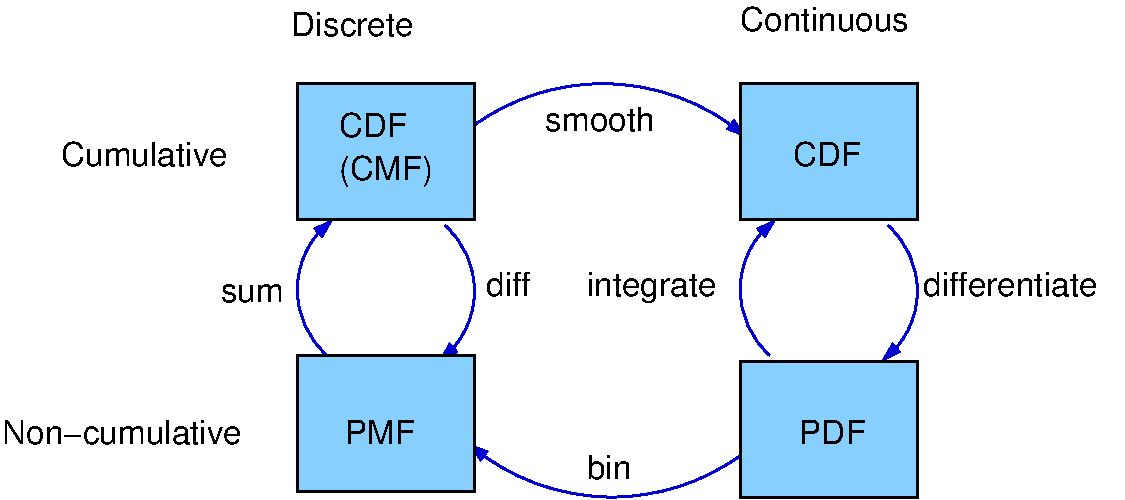
\includegraphics[height=2.2in]{figs/distribution_functions.pdf}}
\caption{Struktura vzájemných souvislostí distribučních funkcí.}
\label{dist_framework}
\end{figure}

Dosud jsme se setkali s PMFs, CDFs a PDFs; pojďme si je krátce připomenout.
Obrázek~\ref{dist_framework} ukazuje, jaké jsou mezi těmito funkcemi vzájemné vztahy.
\index{PMF}

Začali jsme pravděpodobnostními funkcemi (PMFs), které znázorňují pravděpodobnosti pro množinu diskrétních hodnot. Abychom se od PMF propracovali k distribuční funkci (CDF), vypočítali jsme kumulativní součet. Abychom byli konzistentní, diskrétní CDF by se měla nazývat kumulativní funkce (cumulative mass
function -- CMF), ale pokud je mi známo, tak tento pojem nikdo nepoužívá.
\index{CDF}

Abyste se dostali od CDF k hustotě pravděpodobnosti (PMF), můžete vypočítat rozdíly v kumulativních pravděpodobnostech.
\index{PDF}

Podobně pak PDF je derivací spojité CDF; nebo ekvivalentně CDF je integrálem PDF.
Nezapomeňte ale, že PDF přiděluje hodnotám hustoty pravděpodobnosti. Abyste získali pravděpodobnost, musíte integrovat.
\index{diskrétní}
\index{spojitý}

Abyste se od diskrétního rozdělení dostali ke spojitému, můžete provést různé druhy vyrovnání dat. Jednou z forem vyrovnání dat je předpokládat, že data pocházejí z analytického spojitého rozdělení (jako je exponenciální nebo normální rozdělení) a odhadnout parametry takového rozdělení. Přesně tomu se věnuje Kapitola~\ref{estimation}.
\index{exponenciální rozdělení}
\index{rozdělení!exponenciální}
\index{normální rozdělení}
\index{rozdělení!normální}
\index{Gaussovo rozdělení}
\index{rozdělení!Gaussovo}
\index{třída}

Jestliže rozdělíte PDF do souboru tříd, můžete vygenerovat PMF, která je alespoň aproximací PDF. Tuto techniku používáme v Kapitole~\ref{estimation} k získání bayesovského odhadu.
\index{bayesovský odhad}
\index{odhad!bayesovský}

\begin{exercise}
Napište funkci s názvem {\tt MakePmfFromCdf}, která přijme objekt Cdf a vrátí odpovídající objekt Pmf.

Řešení tohoto cvičení najdete v {\tt thinkstats.com/Pmf.py}.
\index{{\tt pmf.py}@{\tt Pmf.py}}

\end{exercise}

\section{\protect\raggedright Glosář}

\begin{description}

\item[šikmost (skewness):] Vlastnost rozdělení; intuitivně, se jedná míru asymetričnosti rozdělení.
\index{šikmost}

\item[robustní (robust):] Statistická charakteristika je robustní, jestliže je relativně imunní vůči působení odlehlých hodnot.
\index{robustní}

\item[iluze nadřazenosti (illusory superiority):] Lidský sklon představovat si, že jsem lepší než průměr.
\index{iluze nadřazenosti}
\index{klam!iluze nadřazenosti}

\item[náhodná proměnná (random variable):] Objekt, který představuje náhodný proces.
\index{náhodná proměnná}
\index{proměnná!náhodná}

\item[náhodná hodnota (random variate):] Hodnota vygenerovaná náhodným procesem.
\index{náhodná hodnota}
\index{hodnota!náhodná}

\item[hustota pravděpodobnosti (PDF) (probability density function):] Hustota pravděpodobnosti je derivátem spojité CDF.
\index{PDF}
\index{hustota pravděpodobnosti}

\item[konvoluce (convolution):] Operace, která vypočítá rozdělení součtu hodnot ze dvou rozdělení.
\index{konvoluce}

%\item[Chi-squared distribution:] The distribution of the sum of squared
%values from a normal distribution.

%\item[Degrees of freedom:] The number of values in a sample that are
%free to vary.

\item[centrální limitní věta (Central Limit Theorem):] ``Nejvyšší zákon Chaosu'', podle Sira Francise Galtona, průkopníka statistiky.
\index{centrální limitní věta}
\index{Galton, Francis}
\index{nejvyšší zákon chaosu}

\end{description}


\chapter{Testování hypotéz}
\label{testing}
\index{testování hypotéz}
\index{pozorované zjištění}

Při průzkumu dat ze souboru NSFG jsme narazili na řadu ``pozorovaných zjištění'',
včetně několika rozdílů mezi prvorozenými a ostatními dětmi. Tato zjištění jsme dosud brali za bernou minci,
v této kapitole je ale, konečně, podrobíme zkoušce.
\index{Národní šetření růstu rodin -- National Survey of Family Growth}
\index{NSFG}

Základní otázkou, na kterou chceme najít odpověď, je, zda jsou tato zjištění skutečná. Například jestliže vypozorujeme
rozdíl v průměrné délce těhotenství u prvorozených a ostatních dětí, chceme zjistit, jestli je daný rozdíl skutečný, nebo jestli k němu došlo náhodně.
\index{délka těhotenství}

Ukazuje se, že tuto otázku není lehké zodpovědět přímo, a tak budeme postupovat
ve dvou krocích. Nejprve otestujeme, zda je dané zjištění {\bf
  významné}, a poté se pokusíme výsledek interpretovat jako odpověď na naši původní otázku.
 \index{významný}

V kontextu statistiky se pojem ``významný'' používá v technickém významu, který se liší od způsobu užití tohoto slova v běžném jazyce.
Jak jsme uvedli v dřívější definici, pozorované zjištění je statisticky významné, jestliže je nepravděpodobné, že je dílem náhody.
\index{náhoda}

Abychom to upřesnili, je potřeba zodpovědět tři otázky:

\begin{enumerate}

\item Co máme na mysli pod pojmem ``náhoda''?

\item Co máme na mysli pod pojmem ``nepravděpodobné''?

\item Co myslíme na mysli pod pojmem ``zjištění''?

\end{enumerate}

Všechny tři tyto otázky jsou těžší, než se zdá. Nicméně existuje obecná struktura, kterou lidé používají k otestování statistické významnosti:

\begin{description}

\item[Nulová hypotéza:] {\bf Nulová hypotéza} představuje model systému vycházející z předpokladu, že pozorované zjištění bylo ve skutečnosti dílem náhody.
\index{nulová hypotéza}

\item[p-hodnota:] {\bf P-hodnota} je pravděpodobnost pozorovaného zjištění při nulové hypotéze.
\index{p-hodnota}

\item[Interpretace:] Na základě p-hodnoty dospějeme k závěru, že zjištění buď je, nebo není statisticky významné.
\end{description}

Tento proces se nazývá {\bf testování hypotéz}.  Opírá se o obdobnou logiku jako důkaz sporem. Abychom ověřili správnost matematického výroku A, předpokládáme dočasně, že výrok A není pravdivý. Jestliže tento předpoklad vede ke sporu, vyvodíme z toho, že výrok A musí být ve skutečnosti pravdivý.
\index{důkaz sporem}

Obdobně pak, abychom otestovali hypotézu jako například "Toto zjištění je skutečné``, předpokládáme dočasně, že není. Tento předpoklad představuje nulovou hypotézu. Na základě tohoto předpokladu vypočteme pravděpodobnost
pozorovaného zjištění, tedy p-hodnotu. Je-li p-hodnota dostatečně nízká, vyvodíme z toho závěr, že je nepravděpodobné, aby nulová hypotéza byla pravdivá.


\section{\protect\raggedright Testování rozdílu v průměrech}
\index{průměr, rozdíl}

Jednou z nejsnadněji otestovatelných hypotéz je pozorovaný rozdíl v průměru mezi dvěma skupinami.
V rámci dat v souboru NSFG jsme zjistili, že průměrná délka těhotenství u prvorozených dětí byla mírně větší a průměrná porodní hmotnost mírně menší. Teď se podíváme na to, zda jsou tato zjištění významná.
\index{Národní šetření růstu rodin -- National Survey of Family Growth}
\index{NSFG}
\index{délka těhotenství}

Pro tyto příklady je nulová hypotéza tvrzení, že rozdělení pro tyto dvě skupiny jsou totožná a že pozorovaný rozdíl je dílem náhody.
\index{nulová hypotéza}

Pro účely výpočtu p-hodnot zjistíme celkové rozdělení pro všechny porody živých dětí (prvorozené a ostatní děti), vygenerujeme náhodné výběrové soubory o stejném rozsahu jako pozorované výběrové soubory a vypočítáme rozdíl v průměrech při nulové hypotéze.
\index{p-hodnota}

Jestliže vygenerujeme velký počet výběrových souborů, můžeme spočítat, jak často je rozdíl v průměrech (v důsledku náhody) stejně velký nebo větší než skutečně pozorovaný rozdíl. Tento podíl představuje p-hodnotu.

Pokud jde o délku těhotenství, pozorovali jsme \n~=~4413 prvorozených dětí a \m~=~4735
ostatních dětí, rozdíl v průměru byl přitom \mydelta~=~0,078 týdnů.  Abych docílil aproximace p-hodnoty tohoto zjištění, sloučil jsem rozdělení, vygeneroval jsem výběrové soubory o rozsahu
 \n~a \m~a vypočítal jsem rozdíl v průměru.
\index{resampling}

Toto je další příklad procesu zvaného resampling, protože vybíráme náhodný vzorek
ze souboru dat, který je sám o sobě výběrem z obecné populace.
Vypočítal jsem rozdíly pro 1000 výběrových párů.
Obrázek~\ref{length_deltas_cdf} ukazuje jejich rozdělení.

\begin{figure}
% hypothesis.py
\centerline{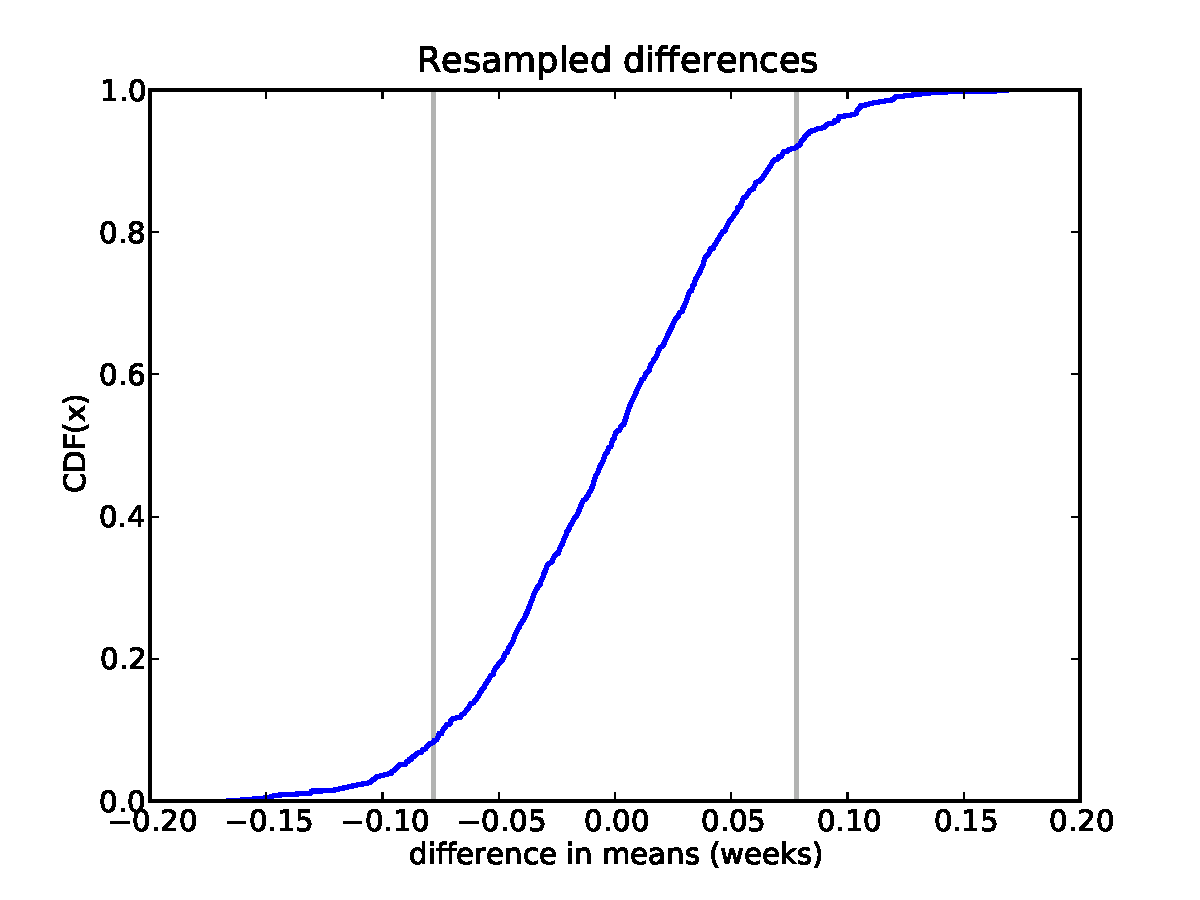
\includegraphics[height=2.5in]{figs/length_deltas_cdf.pdf}}
\caption{CDF rozdílu v průměru pro resamplovaná data.}
\label{length_deltas_cdf}
\end{figure}

Rozdíl v průměru se blíží 0, jak se dá očekávat u vzorků ze stejného rozdělení. Svislé čáry představují oříznuté okraje, kde
\x~=~\minus\mydelta~nebo \x~=~\mydelta.

Z 1000 výběrových párů bylo 166, kdy byl rozdíl v průměru (kladný nebo záporný) stejně velký nebo
větší než \mydelta, takže p-hodnota je přibližně 0,166.  Jinými slovy, očekáváme, že se setkáme se zjištěním, které bude stejně velké jako \mydelta~přibližně v 17 \% případů, dokonce i když je skutečné rozdělení pro obě skupiny stejné.

Pozorované zjištění tudíž není příliš pravděpodobné, ale je dostatečně nepravděpodobné? Této otázce se budu věnovat v další části.

\begin{exercise}
V souboru dat NSFG je rozdíl v průměrné hmotnosti u prvorozených dětí 2,0 unce. Vypočtěte p-hodnotu tohoto rozdílu.
\index{Národní šetření růstu rodin -- National Survey of Family Growth}
\index{NSFG}

Nápověda: U tohoto druhu resamplingu je důležité provádět výběr s opakováním, proto byste měli použít
 {\tt random.choice} spíše než {\tt random.sample} (viz Oddíl~\ref{random}).
\index{resampling}
\index{modul random}

Můžete začít kódem, který jsem použil k vygenerování výsledků v tomto oddílu. Můžete si jej stáhnout z \url{http://thinkstats.com/hypothesis.py}.
\index{{\tt hypothesis.py}}

\end{exercise}


\section{\protect\raggedright Výběr hladiny významnosti}
\label{threshold}
\index{hladina významnosti}

Při testování hypotéz se musíme mít na pozoru před dvěma druhy chyb.
\index{falešně pozitivní}
\index{falešně negativní}
\index{chyba, I. druhu}
\index{chyba, II. druhu}

\begin{itemize}

\item Chyba I. druhu, označovaná také jako {\bf falešně pozitivní}, nastává, když přijmeme hypotézu, která je ve skutečnosti nepravdivá; neboli jestliže považujeme nějaké zjištění za významné, když je ve skutečnosti dílem náhody.

\item Chyba II. druhu, označovaná také jako {\bf falešně negativní}, nastává, když zamítneme hypotézu, která je ve skutečnosti pravdivá; neboli jestliže nějaký atribut připíšeme náhodě, když je skutečný.


\end{itemize}

Nejběžnější přístup k testování hypotéz spočívá v tom, že se zvolí hladina významnosti\footnote{Známá také jako ``kritérium významnosti''.},
\myalpha, pro p-hodnotu a jako významná jsou přijata jakákoliv zjištění s p-hodnotou menší než \myalpha.  Běžnou volbou v případě \myalpha~je 5 \%.
Na základě tohoto kritéria není pozorovaný rozdíl v délce těhotenství u prvorozených dětí významný, zatímco rozdíl v hmotnosti je.
\index{kritérium významnosti}
\index{délka těhotenství}

U tohoto typu testování hypotéz můžeme vypočítat pravděpodobnost chyby I. druhu explicitně: Jedná se o \myalpha.

Abyste pochopili, proč tomu tak je, uvažujte o definici chyby I. druhu -- pravděpodobnost přijetí hypotézy, která je nepravdivá -- a o definici p-hodnoty
-- pravděpodobnost vygenerování naměřeného zjištění, jestliže je hypotéza nepravdivá.

Když dáme tyto dvě definice dohromady, můžeme si položit otázku: Je-li hypotéza nepravdivá, jaká je pravděpodobnost vygenerování naměřeného zjištění, které bude považováno za významné s hladinou \myalpha?  Odpověď zní
\myalpha.

Pravděpodobnost chyby I. druhu můžeme snížit snížením hladiny významnosti. Například jestliže je hladina významnosti 1 \%, existuje pouze 1\% pravděpodobnost chyby I. druhu.

Není to však zcela zadarmo: Snížení hladiny významnosti znamená zvýšení důkazního standardu, což zvyšuje pravděpodobnost zamítnutí platné hypotézy.

Obecně existuje mezi chybami I. a II. druhu vzájemné vyvažování. Jediný způsob, jak snížit obě zároveň, je zvýšit rozsah vzorku (nebo, v některých případech, snížit chybu měření).
\index{rozsah vzorku}

\begin{exercise}
K prověření vlivu rozsahu výběru na p-hodnotu, uvažujte o tom, co se stane, když odstraníte polovinu dat ze souboru NSFG.  Nápověda: Použijte {\tt
  random.sample}.  Co když odstraníte tři čtvrtiny dat, a tak dále?
\index{Národní šetření růstu rodin -- National Survey of Family Growth}
\index{NSFG}

Jaký je nejmenší rozsah výběru, u něhož je rozdíl v průměrné porodní hmotnosti stále ještě významný při
\myalpha~=~5 \%?  O kolik větší musí být rozsah výběru při
\myalpha~=~1 \%?

Můžete začít kódem, který jsem použil k vygenerování výsledků v tomto oddílu. Je ke stažení zde:  \url{http://thinkstats.com/hypothesis.py}.
\index{{\tt hypothesis.py}}

\end{exercise}


\section{\protect\raggedright Definování zjištění}

Stane-li se něco neobvyklého, lidé často říkají něco jako:
``Teda!  Jaká byla pravděpodobnost, že se {\em tohle} stane?''  Tato otázka dává smysl, protože intuitivně vnímáme, že některé věci jsou pravděpodobnější než jiné. Při podrobnějším přezkoumání tato intuice ale vždy neobstojí.
\index{pravděpodobnost}
\index{mince}

Předpokládejme například, že hodím 10krát mincí a po každém hodu zapíšu P, když padne panna, a O, když padne orel.
Bude-li výsledkem sekvence OPPOPOOOPP, asi to nikoho příliš nepřekvapí.  Jestliže bude ale výsledek vypadat takto:
PPPPPPPPPP, asi byste reagovali slovy jako ``Teda!  Jaká byla pravděpodobnost, že se
{\em tohle} stane?''

V tomto příkladu je ale pravděpodobnost obou sekvencí stejná: jedna ku 1024.  A to stejné platí pro jakoukoliv jinou sekvenci. Takže ptáme-li se:  ``Jaká byla pravděpodobnost, že se {\em tohle} stane?'', musíme si dát pozor na to, co myslíme tím ``tohle''.

Pro data ze souboru NSFG jsem definoval zjištění jako ``rozdíl v průměru
(kladný nebo záporný) stejný nebo větší než \mydelta.''  Tím, že jsem provedl tuto volbu, jsem se rozhodl hodnotit velikost rozdílu bez ohledu na znaménko.
\index{Národní šetření růstu rodin -- National Survey of Family Growth}
\index{NSFG}

Takovýto test se nazývá {\bf dvoustranný} test, protože bereme do úvahy obě strany
 (kladnou a zápornou) v rozdělení na Obrázku~\ref{length_deltas_cdf}.  Použitím dvoustranného testu testujeme hypotézu o tom, že existuje významný rozdíl mezi rozděleními, aniž bychom specifikovali znaménko příslušného rozdílu.
\index{jednostranný test}
\index{dvoustranný test}
\index{test!jednostranný}
\index{test!dvoustranný}

Alternativou je pak použití {\bf jednostranného} testu, který se ptá, zda průměr u prvorozených dětí je významně
{\em vyšší} než průměr u ostatních dětí.
Protože je tato hypotéza konkrétnější, je p-hodnota nižší -- v tomto případě je přibližně poloviční.


\section{\protect\raggedright Interpretace výsledku}

V úvodu této kapitoly jsem uvedl, že otázka, na niž chceme najít odpověď, je, zda je pozorované zjištění skutečné.
Začali jsme definicí nulové hypotézy, označované jako \HH\sub{0}, což je hypotéza o tom, že zjištění není skutečné.
Následně jsme definovali p-hodnotu, tedy
\Prob(\E|\HH\sub{0}), kde \E~je zjištění stejné nebo větší než pozorované zjištění. Poté jsme vypočetli p-hodnoty a porovnali jsme je s hladinou \myalpha.

To je užitečný krok, ale nepřináší odpověď na původní otázku, tedy na to, zda je zjištění skutečné. Existuje několik způsobů interpretace výsledku testu hypotézy:

\begin{description}

\item[Klasický:] Při klasickém testování hypotéz platí, že je-li p-hodnota menší než \myalpha,
můžeme říci, že zjištění je statisticky významné, ale nemůžeme říci, že je skutečné.   Taková formulace je dostatečně opatrná, abychom se vyhnuli ukvapeným závěrům, ale je hluboce neuspokojivá.

\item[Praktický:] V praxi lidé nepostupují takto formálně. Ve většině vědeckých časopisů badatelé uvádí p-hodnoty bez rozpaků a čtenáři si je vykládají jako důkaz o tom, že pozorované zjištění je skutečné. Čím nižší je p-hodnota, tím větší je důvěra v takový závěr.
\index{bayesovská pravděpodobnost}

\item[Bayesovský:] To, co nás skutečně zajímá, je \Prob(\HH\sub{A}|\E),
 kde \HH\sub{A} je hypotéza o tom, že zjištění je skutečné.
  Za použití Bayesovy věty
  %
  \[ P(H_A \given E) = \frac{P(E \given H_A) \spa P(H_A)}{P(E)} \]
  %
  kde \Prob(\HH\sub{A}) je apriorní pravděpodobnost \HH\sub{A} před tím, než jsme zaznamenali příslušné zjištění, \Prob(\E|\HH\sub{A}) je pravděpodobnost zpozorování \E,
  za předpokladu, že zjištění je skutečné, a \Prob(\E) je pravděpodobnost zpozorování \E~při jakékoliv hypotéze. Vzhledem k tomu, že zjištění buď je, nebo není skutečné:

  \Eqn{ \Prob(\E) = \Prob(\E|\HH\sub{A}) \Prob(\HH\sub{A})~+~\Prob(\E|\HH\sub{0}) \Prob(\HH\sub{0}) }

\end{description}

Jako příklad vypočítám \Prob(\HH\sub{A}|E) pro délky těhotenství v rámci NSFG.  Už jsme vypočítali
\Prob(\E|\HH\sub{0})~=~0,166, takže nám zbývá jen vypočítat
\Prob(\E|\HH\sub{A}) a zvolit hodnotu pro apriorní pravděpodobnost.
\index{apriorní pravděpodobnost}
\index{Národní šetření růstu rodin -- National Survey of Family Growth}
\index{NSFG}
\index{délka těhotenství}

Pro účely výpočtu \Prob(\E|\HH\sub{A}) předpokládáme, že je zjištění skutečné
-- tedy že rozdíl v průměrné délce trvání, \mydelta, je ve skutečnosti roven námi vypozorovanému výsledku
0,078.  (Tento způsob formulace \HH\sub{A}~je trochu podvodný.
Tento problém vysvětlím a nápravu zjednám v dalším oddílu.)

Vygenerováním 1000 výběrových párů, vždy jednoho z každého rozdělení, jsem odhadl, že
\Prob(E|\HH\sub{A})~=~0,494.  Při apriorní pravděpodobnosti
\Prob(\HH\sub{A})~=~0,5 je aposteriorní pravděpodobnost \HH\sub{A} rovna 0,748.
\index{aposteriorní pravděpodobnost}
\index{aktualizace}

Jestliže apriorní pravděpodobnost \HH\sub{A}~je 50 \%, aktualizovaná pravděpodobnost, se zohledněním důkazů z tohoto souboru dat, je téměř 75 \%.  Dává smysl, že aposteriorní pravděpodobnost je vyšší, neboť data poskytují určitou podporu pro danou hypotézu. Mohlo by se ale zdát překvapivé, že ten rozdíl je tak velký, zejména v situaci, kdy jsme zjistili, že rozdíl v průměrech nebyl statisticky významný.

Ve skutečnosti není metoda, kterou jsem použil v tomto oddílu, tak docela správná a projevuje se u ní tendence přeceňovat význam důkazů. V dalším oddílu provedu korekci této tendence.

\begin{exercise}
Na základě dat z NSFG určete, jaká je aposteriorní pravděpodobnost, že rozdělení porodních hmotností se liší u prvorozených a ostatních dětí.
\index{porodní hmotnost}
\index{hmotnost!porodní}
\index{Národní šetření růstu rodin -- National Survey of Family Growth}
\index{NSFG}

Můžete začít kódem, který jsem použil k vygenerování výsledků v tomto oddílu. Můžete si jej stáhnout zde:  \url{http://thinkstats.com/hypothesis.py}.
\index{{\tt hypothesis.py}}

\end{exercise}


\section{\protect\raggedright Křížová validace}
\index{křížová validace}

V předchozím příkladu jsme použili k formulaci hypotézy
\HH\sub{A} soubor dat a pak jsme tentýž soubor dat použili k jejímu otestování. To není dobrý nápad; může se totiž velmi snadno stát, že vygenerujeme zavádějící výsledky.

Problém spočívá v tom, že i když je nulová hypotéza pravdivá, je pravděpodobné, že mezi libovolnými dvěma skupinami existuje nějaký rozdíl, \mydelta, čistě náhodně.
Použijeme-li zjištěnou hodnotu \mydelta~k formulaci hypotézy, je pravděpodobné, že
\Prob(\HH\sub{A}|\E) bude vysoká, i když je \HH\sub{A}~nepravdivá.

S tímto problémem se můžeme vypořádat s pomocí {\bf křížové validace}, která používá jeden soubor dat k výpočtu \mydelta~a {\em jiný} soubor dat k vyhodnocení \HH\sub{A}. První soubor dat se nazývá {\bf trénovací množina}, druhý pak
{\bf testovací množina}.
\index{trénovací množina}
\index{testovací množina}
\index{kohorta}
\index{cyklus}

V rámci studie jako je NSFG, která v každém cyklu sleduje jinou kohortu, můžeme použít jeden cyklus pro trénování a jiný pro testování. Nebo můžeme data rozdělit do podmnožin (náhodně), a pak použít jednu pro trénování a druhou pro testování.
\index{Národní šetření růstu rodin -- National Survey of Family Growth}
\index{NSFG}

Já jsem použil druhý přístup, kdy jsem data z Cyklu 6 rozdělil zhruba na dvě poloviny. Provedl jsem test několikrát s různým náhodným rozdělením. Průměrná aposteriorní pravděpodobnost byla \Prob(\HH\sub{A}|\E)~=~0,621.
Podle očekávání je dopad důkazů menší, částečně v důsledku menšího rozsahu vzorku v testovací množině, ale také v důsledku toho, že už nepoužíváme stejný soubor dat pro trénování i testování.

% t = [0.656, 0.622, 0.511, 0.651, 0.665]
% sum(t)/len(t)


\section{\protect\raggedright Vyjadřování bayesovských pravděpodobností}
\index{bayesovská pravděpodobnost}

V předešlé části jsme zvolili apriorní pravděpodobnost \Prob(\HH\sub{A})~=~0,5.
Máme-li množinu hypotéz a nemáme přitom žádný důvod domnívat se, že jedna z nich je pravděpodobnější než ostatní, je obvyklé, že každé z nich přidělíme stejnou pravděpodobnost.

Někteří lidé mají vůči bayesovským pravděpodobnostem výhrady, protože jsou závislé na apriorních pravděpodobnostech a může se stát, že se nenajde shoda ohledně toho, jaká apriorní pravděpodobnost je správná. Pro ty, kdo očekávají, že vědecké výsledky budou objektivní a univerzální, je tato vlastnost hluboce znepokojivá.
\index{subjektivní přesvědčení}
\index{přesvědčení}
\index{zastínit}
\index{konvergence}

Jednou možnou odpovědí na tuto výhradu je to, že v praxi mají silné důkazy tendenci zastínit efekt apriorní pravděpodobnosti, takže lidé, kteří začnou s různými apriorními pravděpodobnostmi, nakonec konvergují ke stejné aposteriorní pravděpodobnosti.
\index{věrohodnostní poměr}
\index{Bayesův faktor}

Další možností je uvádět pouze {\bf věrohodnostní poměr}, \Prob(E
| \HH\sub{A}) ~/~ \Prob(\E|\HH\sub{0}), namísto aposteriorní pravděpodobnosti.
Tímto způsobem si čtenáři mohou dosadit jakoukoliv apriorní pravděpodobnost a vypočítat svoje vlastní aposteriorní pravděpodobnosti. Věrohodnostní poměr se někdy označuje jako Bayesův faktor (viz
\url{http://wikipedia.org/wiki/Bayes_factor}).

\begin{exercise}
Jestliže jste určili apriorní pravděpodobnost hypotézy \HH\sub{A} jako 0,3 a objeví se nové důkazy, v jejichž světle vyjde věrohodnostní poměr na 3 ve vztahu k nulové hypotéze \HH\sub{0}, jaká je v tomto případě aposteriorní pravděpodobnost pro \HH\sub{A}?
\index{nulová hypotéza}

% 0.3 * 3 / (0.3 * 3 + 0.7) = 0.6

\end{exercise}


\begin{exercise}
Toto cvičení je převzato z MacKay, {\em Information
  Theory, Inference, and Learning Algorithms}:
\index{MacKay, David}

\begin{quote}

Na místě činu zanechali stopy své krve dva lidé. Oliver, který je podezřelý, je podroben
testu, který určí jeho krevní typ jako 0. Ukáže se, že ony dvě stopy krve odpovídají typu 0 (v místní populaci se jedná o běžný typ, s  60\% četností) a dále typu AB (vzácný typ, s četností 1 \%).  Poskytují tato data (krevní typy nalezené na místě činu) důkaz svědčící ve prospěch tvrzení, že Oliver byl jedním ze dvou lidí, jejichž krev byla nalezena na místě činu?

\end{quote}

Nápověda: Vypočítejte věrohodnostní poměr pro tento důkaz; jestliže je větší než
1, pak tento důkaz svědčí ve prospěch uvedeného tvrzení. Řešení a diskusi najdete na straně 55
MacKayovy knihy.
\index{věrohodnost}

\end{exercise}


\section{\protect\raggedright Chí-kvadrát test}
\index{chí-kvadrát test}

V Oddílu~\ref{threshold} jsme dospěli k závěru, že pozorovaný rozdíl v průměrné délce těhotenství u prvorozených a ostatních
dětí nebyl významný. Avšak v Oddílu ~\ref{relative.risk}, když jsme spočítali relativní riziko, jsme zjistili, že u prvorozených dětí existuje větší pravděpodobnost, že se narodí předčasně, menší pravděpodobnost, že se narodí načas, a větší pravděpodobnost, že se narodí se zpožděním.
\index{relativní riziko}
\index{délka těhotenství}

Možná mají tedy tato rozdělení stejný průměr a různý rozptyl. Mohli bychom otestovat významnost rozdílu v rozptylu, ale rozptyl je méně robustní charakteristika než průměr a testování hypotéz s ohledem na rozptyl obvykle nepřináší kýžené výsledky.
\index{průměr}
\index{rozptyl}
\index{hypotéza}

Alternativou je otestovat hypotézu, která odráží konkrétní zjištění tak, jak je pozorováno, příměji. Neboli hypotézu o tom, že u prvorozených dětí existuje větší pravděpodobnost, že se narodí předčasně, menší pravděpodobnost, že se narodí načas, a větší pravděpodobnost, že se narodí se zpožděním.

Postup spočívá v pěti jednoduchých krocích:

\begin{enumerate}

\item Definujeme množinu kategorií, označovaných jako {\bf políčka}, do nichž by každé z dětí mohlo spadat. V tomto příkladu máme šest políček, protože existují dvě skupiny (prvorozené a ostatní děti) a tři třídy (předčasně, načas a se zpožděním narozené).
 \index{políčko}

Použiji definice z Oddílu~\ref{relative.risk}: Dítě se narodí předčasně, jestliže přijde na svět v průběhu 37. týdne nebo dříve, načas, jestliže se narodí v průběhu 38., 39. nebo 40. týdne, a se zpožděním, jestliže se narodí v průběhu 41. týdne nebo později.

\item Spočítáme počet dětí očekávaných v každém políčku. Při nulové hypotéze předpokládáme, že rozdělení jsou pro obě skupiny stejná, takže můžeme vypočítat úhrnné pravděpodobnosti:
  \Prob(předčasně), \Prob(načas) a \Prob(se zpožděním).

Pro prvorozené děti máme \n~=~4413 vzorků, takže při nulové hypotéze očekáváme \n~\Prob(předčasně) prvorozených dětí, které se narodí předčasně, \n~\Prob(načas), které se narodí načas atd.  Obdobně pak máme \m~=~4735
ostatních dětí, takže očekáváme \m~\Prob(předčasně) ostatních dětí, které se narodí předčasně atd.

\item Pro každé políčko spočítáme odchylku, neboli rozdíl mezi zjištěnou hodnotou, \OO\sub{i}, a očekávanou hodnotou, \E\sub{i}.
\index{testová statistika}
\index{statistika chí-kvadrát}

\item Vypočteme určitou míru celkové odchylky; tato veličina se nazývá {\bf testová statistika}.  Nejběžnější volbou je statistika chí-kvadrát:
%
\[ \chi^2 = \sum_i \frac{(O_i - E_i)^2}{E_i} \]
%
%% Consider using upper case chi, which is more strictly correct,
%% but harder to distinguish from X.

\item K výpočtu p-hodnoty můžeme použít simulaci Monte Carlo, což představuje pravděpodobnost zjištění statistiky chí-kvadrát, která bude stejně vysoká jako hodnota zjištěná při nulové hypotéze.
\index{simulace!Monte Carlo}
\index{Monte Carlo}

\end{enumerate}

Použijeme-li statistiku chí-kvadrát, tento proces se označuje jako {\bf chí-kvadrát test} nebo také {\bf test dobré shody}.  Jedním ze znaků chí-kvadrát testu je, že rozdělení testové statistiky lze vypočítat analyticky.
\index{chí-kvadrát test}
\index{analýza}

Za použití dat ze souboru NSFG jsem vypočítal \mychi\super{2}~=~91,64, přičemž takovýto výsledek by se náhodně vyskytl přibližně v jednom případě z 10 000.  Vyvozuji z toho, že tento výsledek je statisticky významný, s jedním upozorněním -- opět jsme použili stejný soubor dat pro exploraci i testování. Bylo by dobré potvrdit tento výsledek za použití jiného souboru dat.
\index{Národní šetření růstu rodin -- National Survey of Family Growth}
\index{NSFG}

Kód, který jsem použil v tomto oddílu, si můžete stáhnout z
\url{http://thinkstats.com/chi.py}.
\index{{\tt chi.py}}

% See \url{http://en.wiktionary.org/wiki/voila}!


\begin{exercise}
Představte si, že provozujete kasino a máte podezření na jednoho ze zákazníků, že kostku, kterou dává k dispozici kasino, vyměnil za vlastní ``podvrženou kostku;'' tedy takovou, se kterou bylo manipulováno tak, aby jedna ze stran padala častěji než ostatní. Zadržíte tedy domnělého podvodníka a zabavíte příslušnou kostku, teď ale musíte prokázat, že byla podvržená.
\index{kasino}
\index{kostky}
\index{podvržená kostka}

Hodíte kostkou 60krát a dostanete následující výsledky:

\begin{center}
\begin{tabular}{|l|c|c|c|c|c|c|}
\hline
Hodnota     &  1  &  2  &  3  &  4  &  5  &  6  \\
\hline
\hline
Četnost &  8  &  9  &  19  &  6  &  8  &  10  \\
\hline
\end{tabular}
\end{center}

Jaká je statistika chí-kvadrát pro tyto hodnoty? Jaká je pravděpodobnost, že se takto vysoká hodnota chí-kvadrát vyskytne náhodně?

\end{exercise}




\section{\protect\raggedright Účinný resampling}
\index{resampling}

Čtenář této knihy s předchozí znalostí statistiky se zřejmě zasmál, když uviděl Obrázek~\ref{length_deltas_cdf}, protože jsem použil velké výpočetní síly k simulaci něčeho, na co jsem mohl přijít analyticky.
\index{analýza}
\index{délka těhotenství}

Je zřejmé, že matematická analýza není hlavním předmětem této knihy. Jsem ochoten používat počítače k tomu, abych na věci přicházel ``hloupým'' způsobem, protože jsem přesvědčen o tom, že pro začátečníky je jednodušší porozumět simulacím a je také jednodušší demonstrovat, že jsou správné. A tak pokud provedení simulace netrvá příliš dlouho, nemám žádné výčitky kvůli tomu, že jsem přeskočil analýzu.

Nicméně existují situace, kdy trochu analýzy může člověku ušetřit hodně výpočtů a Obrázek
~\ref{length_deltas_cdf} je jedním z těchto případů.
\index{průměr, rozdíl}

Určitě si vzpomínáte, že jsme testovali pozorovaný rozdíl v průměrné délce těhotenství pro \n~=~4413 prvorozených dětí a \m~=~4735 ostatních dětí.  Dospěli jsme k úhrnnému rozdělení pro všechny děti, vybrali jsme vzorky o rozsahu \n~a
\m~a vypočítali jsme rozdíl ve výběrových průměrech.
\index{výběrový průměr}

Místo toho jsme mohli přímo vypočítat rozdělení rozdílu ve výběrových průměrech. Pro začátek uvažujte o tom, co znamená výběrový průměr: vybereme \n~vzorků z rozdělení, sečteme je a výsledek vydělíme \n.  Jestliže má vzorek průměr \mymu~a rozptyl \sigmasq, pak dle centrální limitní věty víme, že součet vzorků je \mynormal (\n \mymu, \n \sigmasq).
\index{normální rozdělení}
\index{rozdělení!normální}
\index{Gaussovo rozdělení}
\index{rozdělení!Gaussovo}

Abychom zjistili rozdělení výběrových průměrů, musíme se odvolat na jednu z vlastností normálního rozdělení: jestliže \X~je
\mynormal (\mymu, \sigmasq),

\Eqn{ \mya\X~+~\myb~\mysim~\mynormal(\mya \mymu~+~\myb, \mya\super{2} \sigmasq) }

Když provedeme dělení \n, \mya~=~1/\n~ a \myb~=~0, pak

\X/\n~\mysim~\mynormal(\mymu /\n, \sigmasq/ \n\super{2})

Rozdělení výběrového průměru je tedy \mynormal (\mymu, \sigmasq/\n).

Abychom získali rozdělení rozdílu mezi dvěma výběrovými průměry, odvoláme se na další vlastnost normálního rozdělení: jestliže \X\sub{1} je
\mynormal (\mymu\sub{1}, \mysigma\sub{1}\super{2}) a \X\sub{2} je
\mynormal (\mymu\sub{2}, \mysigma\sub{2}\super{2}),
%
\[ aX_1 + bX_2 \sim \normal(a\mu_1 + b\mu_2,
                                 a^2\sigma_1^2 + b^2\sigma_2^2) \]
%
Pak jako speciální případ:
%
\[ X_1 - X_2 \sim \normal(\mu_1 - \mu_2,
                               \sigma_1^2 + \sigma_2^2) \]
%
Dáme-li to vše dohromady, dospějeme k závěru, že vzorek na Obrázku~\ref{length_deltas_cdf} je vybrán z
\mynormal (0, \f \sigmasq), kde \f~=~1/\n~+~1/\m.  Po dosazení
\n~=~4413 a \m~=~4735 očekáváme, že rozdíl ve výběrových průměrech bude \mynormal (0, 0,0032).
\index{p-hodnota}

Můžeme použít {\tt erf.NormalCdf} k výpočtu p-hodnoty pozorovaného rozdílu v průměrech:
%
\begin{verbatim}
delta = 0.078
sigma = math.sqrt(0.0032)
left = erf.NormalCdf(-delta, 0.0, sigma)
right = 1 - erf.NormalCdf(delta, 0.0, sigma)
\end{verbatim}

Součet levé a pravé strany je p-hodnota, 0,168, což je velmi blízko našemu odhadu na základě resamplingu, který byl 0,166.
Kód, který jsem použil v tomto oddílu, si můžete stáhnout z
\url{http://thinkstats.com/hypothesis_analytic.py}
\index{{\tt hypothesis\_analytic.py}}

\section{\protect\raggedright Síla}
\index{síla}

Je-li výsledek testování hypotézy negativní (tj. zjištění není statisticky významné), můžeme z toho vyvodit závěr, že zjištění není skutečné? To záleží na síle testu.

Statistická {\bf síla} je pravděpodobnost, že test bude pozitivní, jestliže je nulová hypotéza nepravdivá. Obecně závisí síla testu na rozsahu vzorku, velikosti zjištění a hladině \myalpha.

\begin{exercise}
Jaká je síla testu v Oddílu~\ref{threshold}, za použití
\myalpha~=~0,05 a předpokladu, že skutečný rozdíl mezi průměry je 0,078 týdnů?

Sílu můžete odhadnout vygenerováním náhodných vzorků z rozdělení s daným rozdílem v průměru, otestováním pozorovaného rozdílu v průměru a spočítáním počtu pozitivních testů.

Jaká je síla testu s \myalpha~=~0,10?

\end{exercise}

Jedním ze způsobů, jak uvádět sílu testu, vedle negativního výsledku, je tvrzení na způsob tohoto: ``Pokud by bylo pozorované zjištění stejně velké jako \x, tento test by zamítl nulovou hypotézu s pravděpodobností \p.''


%\section{\protect\raggedright Discussion}

%Pitfalls:

%1) Exploring and then testing

%2) Multiple tests

%3) Publication bias


%Solutions:

%1) two phases: exploratory and testing, on different data (possibly a subset)

%2) Holm-Bonferroni method

%3) publish everything and wait for consensus




\section{\protect\raggedright Glosář}

\begin{description}

\item[významný (significant):] Zjištění je statisticky významné, jestliže je nepravděpodobné, aby k němu došlo náhodně.
\index{významný}

\item[nulová hypotéza (null hypothesis):] Model systému založený na předpokladu, že k pozorovanému zjištění došlo v důsledku náhody.
\index{nulová hypotéza}

\item[p-hodnota (p-value):] Pravděpodobnost toho, že by zjištění mohlo vzniknout náhodně.
\index{p-hodnota}

\item[testování hypotéz (hypothesis testing):] Proces určování, zda je pozorované zjištění statisticky významné.
\index{testování hypotéz}

\item[chyba I. druhu (type I error) (falešně pozitivní (false positive)):] Závěr, že zjištění je skutečné, když tomu tak není.
\index{falešně pozitivní}

\item[chyba II. druhu (type II error) (falešně negativní (false negative)):] Závěr, že zjištění vzniklo v důsledku náhody, když tomu tak není.
\index{falešně negativní}

\item[dvoustranný test (two-sided test):] Test, který se ptá: ``Jaká je pravděpodobnost zjištění, které je stejně velké jako pozorované zjištění, ať už je kladné nebo záporné?''

\item[jednostranný test (one-sided test):] Test, který se ptá: ``Jaká je pravděpodobnost zjištění, které je stejně velké jako pozorované zjištění a má také stejné znaménko?''
\index{jednostranný test}
\index{dvoustranný test}
\index{test!jednostranný}
\index{test!dvoustranný}

\item[křížová validace (cross-validation):] Proces testování hypotéz, který využívá jeden soubor dat pro explorační analýzu dat a jiný soubor dat pro testování.
\index{křížová validace}

\item[trénovací množina (training set):] Soubor dat používaný k formulování hypotézy pro testování.
\index{trénovací množina}

\item[testovací množina (testing set):] Soubor dat používaný k testování.
\index{testovací množina}

\item[testová statistika (test statistic):] Statistika používaná k měření odchylky pozorovaného zjištění od toho, co je očekáváno náhodně.
\index{testová statistika}

\item[chí-kvadrát test, test dobré shody (chi-square test):] Test využívající chí-kvadrát statistiku jako testovou statistiku.
\index{chí-kvadrát test}
\index{test!dobré shody}

\item[věrohodnostní poměr (likelihood ratio):] Poměr \Prob(\E|\A) k \Prob(\E|\B)
  pro dvě hypotézy \A~a \B, což je způsob, jak referovat o výsledcích bayesovské analýzy bez spoléhání se na apriorní pravděpodobnost.
 \index{věrohodnostní poměr}

\item[políčko (cell):] Jedná se o kategorie v  chí-kvadrát testu, do kterých jsou údaje rozděleny.
\index{políčko}

\item[síla (power):] Pravděpodobnost, že test zamítne nulovou hypotézu, jestliže je nepravdivá.
\index{síla}

\end{description}



\chapter{Odhadování}
\label{estimation}
\index{odhad}

\section{\protect\raggedright Hra na odhad}

Pojďme si zahrát hru.  Budu si myslet rozdělení a vy musíte uhodnout, o které jde. Začneme něčím jednoduchým a postupně se bude obtížnost zvyšovat.
\index{normální rozdělení}
\index{rozdělení!normální}
\index{Gaussovo rozdělení}
\index{rozdělení!Gaussovo}

{\em Myslím si rozdělení.} Dám vám dvě nápovědy: Jedná se o normální rozdělení a zde je náhodný vzorek vybraný z tohoto rozdělení:

\{\minus0,441, 1,774, \minus0,101, \minus1,138, 2,975, \minus2,138\}

Jaký si myslíte, že je průměr základního souboru, \mymu, tohoto rozdělení?
\index{průměr}
\index{parametr}

Jednou možností je použít k odhadu \mymu~výběrový průměr.  Dosud jsme používali symbol \mymu~jak pro výběrový průměr, tak pro průměr základního souboru/průměr jako parametr, nyní je však odliším tak, že pro výběrový průměr použiji \myxbar. V tomto příkladu je \myxbar~rovno 0,155, takže by bylo rozumné odhadnout, že \mymu~=~0,155.

Tento proces se označuje jako {\bf odhadování} a statistika, kterou jsme použili (výběrový průměr) se nazývá {\bf odhad}.
\index{odhad}

Použití výběrového průměru pro odhadnutí \mymu~je natolik zřejmé, že je obtížné představit si jakoukoliv odpovídající alternativu. Představte si ale, že hru změníme zapojením odlehlých hodnot.
\index{normální rozdělení}
\index{rozdělení!normální}
\index{Gaussovo rozdělení}
\index{rozdělení!Gaussovo}

{\em Myslím si rozdělení.}  Jedná se o normální rozdělení a zde je vzorek sestavený nespolehlivým měřičem, který občas umístí špatně desetinnou čárku.

\{\minus0,441, 1,774, \minus0,101, \minus1,138, 2,975, \minus213,8\}

Jaký je nyní váš odhad \mymu?  Použijete-li výběrový průměr, váš odhad bude
\minus35,12.  Je toto nejlepší možná volba? Jaké jsou alternativy?
\index{odlehlá hodnota}

Jednou možností je určit a vyřadit odlehlé hodnoty a pak spočítat výběrový průměr zbytku. Další možností je použít jako odhad medián.
\index{medián}

To, který odhad nám poslouží nejlépe, závisí na okolnostech (např. zda jsou přítomny odlehlé hodnoty) a také na tom, jaký je účel. Snažíte se minimalizovat chyby, nebo maximalizovat vaši šanci na nalezení správné odpovědi?
\index{chyba}
\index{MSE}
\index{střední kvadratická chyba}

Jestliže se v souboru nevyskytují žádné odlehlé hodnoty, výběrový průměr minimalizuje {\bf střední kvadratickou chybu
(mean squared error -- MSE)}. Jestliže budeme hru mnohokrát opakovat a pokaždé vypočítáme chybu \myxbar~\minus~\mymu, výběrový průměr minimalizuje
%
\[ MSE = \frac{1}{m} \sum (\xbar - \mu)^2 \]
%
Kde \m~je počet opakování hry na odhad (nezaměňovat s \n, což je rozsah výběrového souboru použitého k výpočtu \myxbar).

Minimalizace MSE je pěkná vlastnost, ale není to vždy ta nejlepší strategie. Představte si například situaci, kdy odhadujeme rozdělení rychlostí větru na staveništi. Pokud bude náš odhad příliš nadsazený, může se stát, že konstrukce bude zbytečně naddimenzovaná, čímž se zvýší náklady. Pokud ale bude náš odhad příliš nízký, budova by mohla spadnout. Protože náklady jako funkce chyby jsou asymetrické, minimalizace MSE není nejlepší strategií.
\index{predikce}

Jako další příklad uvažujte situaci, kdy hodím tři šestistranné kostky a požádám vás o předpověď součtu. Jestliže se přesně trefíte, získáte výhru, jinak nedostanete nic. V tomto případě je hodnota, která minimalizuje MSE, 10,5, ale to by byl příšerný odhad. Pro tuto hru potřebujete odhad, který má největší šanci na správnou odpověď, a tím je
{\bf maximálně věrohodný odhad (maximum likelihood estimator -- MLE}). Jestliže zvolíte 10 nebo 11, vaše šance na výhru je 1 ku 8, a to je také nejlepší pozice, jakou můžete mít.
\index{MLE}
\index{maximálně věrohodný odhad}

\begin{exercise}
Napište funkci, která vybere 6 hodnot z normálního rozdělení s \mymu~=~0 a \mysigma~=~1.  K odhadu \mymu~použijte výběrový průměr a vypočtěte chybu \myxbar~\minus~\mymu.  Proveďte funkci 1000krát a vypočtěte MSE.
\index{normální rozdělení}
\index{rozdělení!normální}
\index{Gaussovo rozdělení}
\index{rozdělení!Gaussovo}

Nyní program modifikujte tak, aby použil jako odhad medián. Znovu vypočtěte MSE a porovnejte s MSE pro \myxbar.
\index{průměr}
\index{medián}
\index{MSE}

\end{exercise}


\section{\protect\raggedright Odhadněte rozptyl}
\index{rozptyl}
\index{normální rozdělení}
\index{rozdělení!normální}
\index{Gaussovo rozdělení}
\index{rozdělení!Gaussovo}

{\em Myslím si rozdělení.}  Jedná se o normální rozdělení a zde je (známý) vzorek:

\{\minus0,441, 1,774, \minus0,101, \minus1,138, 2,975, \minus2,138\}

Jaký si myslíte, že je rozptyl, \sigmasq, mého rozdělení?
Opět platí, že zřejmou volbou je použití výběrového rozptylu jako odhadu. K označení výběrového rozptylu budu používat \Ssq, abych jej odlišil od neznámého parametru \sigmasq.
%
\[ S^2 = \frac{1}{n} \sum (x_i - \xbar)^2 \]
%
Pro velké výběrové soubory představuje \Ssq~adekvátní odhad, ale pro malé výběrové soubory bývá příliš nízký. Vzhledem k této nešťastné vlastnosti se označuje jako {\bf zkreslený} odhad.
\index{výběrový rozptyl}
\index{zkreslený odhad}
\index{odhad!zkreslený}
\index{nezkreslený odhad}
\index{odhad!nezkreslený}


Odhad je {\bf nezkreslený}, jestliže očekávaná celková (nebo střední) chyba po mnoha opakováních hry na odhad je
0.
Naštěstí existuje další jednoduchá statistika, která je nezkresleným odhadem \sigmasq:
%
\[ S_{n-1}^2 = \frac{1}{n-1} \sum (x_i - \xbar)^2 \]
%
Největší problém s tímto odhadem je, že jeho název a symbol se používají nekonzistentně. Název ``výběrový rozptyl'' může odkazovat buď k \Ssq~nebo \Snsq~a symbol \Ssq~se používá pro kterýkoliv z nich nebo pro oba.

Zajímá-li vás vysvětlení, proč je \Ssq~zkreslený, a důkaz o tom, že \Snsq~je nezkreslený, podívejte se na
\url{http://wikipedia.org/wiki/Bias_of_an_estimator}.

\begin{exercise}
Napište funkci, která vybere 6 hodnot z normálního rozdělení s \mymu~~=~~0 a \mysigma~~=~~1.  Použijte výběrový rozptyl k odhadu \sigmasq~a vypočtěte chybu \Ssq~\minus~\mysigma\super{2}.
Proveďte funkci 1000krát a vypočtěte střední chybu (ne kvadratickou).
\index{normální rozdělení}
\index{rozdělení!normální}
\index{Gaussovo rozdělení}
\index{rozdělení!Gaussovo}

Nyní program modifikujte, aby použil nezkreslený odhad \Snsq.
Znovu vypočtěte střední chybu a podívejte se, zda konverguje k nule s tím, jak se zvyšuje počet opakování hry.

\end{exercise}


\section{\protect\raggedright Pochopení chyb}
\index{chyba}

Než budeme pokračovat, je důležité vyjasnit si jeden častý zdroj nedorozumění.
Vlastnosti jako MSE a zkreslení jsou dlouhodobá očekávání založená na mnoha opakováních hry na odhad.

Zatímco hru hrajete, neznáte chyby. Tím mám na mysli to, že když vám dám vzorek a požádám vás o odhad parametru, můžete vypočítat hodnotu odhadu, ale nemůžete vypočítat chybu. Pokud byste mohli, pak byste nepotřebovali odhad!

Důvod, proč hovoříme o chybě odhadu, je, abychom popsali chování různých odhadů z dlouhodobého hlediska. V této kapitole provádíme experimenty, jejichž smyslem je prozkoumat toto chování. Tyto experimenty jsou umělé v tom smyslu, že známe skutečné hodnoty parametrů, a tak můžeme vypočítat chyby. Při práci se skutečnými daty ale tyto hodnoty neznáte, a tak nemůžete chyby vypočítat.

Nyní ale zpět ke hře.


\section{\protect\raggedright Exponenciální rozdělení}
\index{exponenciální rozdělení}
\index{rozdělení!exponenciální}

{\em Myslím si rozdělení.}  Jedná se o exponenciální rozdělení a zde je vzorek:

\{5,384, 4,493, 19,198, 2,790, 6,122, 12,844\}

Jaký si myslíte, že je parametr \mylambda~tohoto rozdělení?
\index{parametr}
\index{průměr}

\newcommand{\lamhat}{\hat{\lambda}}
\newcommand{\lamhatmed}{\hat{\lambda}_{1/2}}

Obecně platí, že průměr exponenciálního rozdělení je 1/\mylambda,
takže budeme-li postupovat opačně, mohli bychom zvolit

\Eqn{ $\lamhat$ = 1 / \myxbar }

Je běžnou praxí používat pro odhady zápis se stříškou, takže $\lamhat$ je odhad
\mylambda.  A ne ledajaký odhad; je to také odhad MLE\footnote{Viz
\url{http://wikipedia.org/wiki/Exponential_distribution#Maximum_likelihood}.}.
Chcete-li tedy maximalizovat svoji šanci na přesný odhad \mylambda, pak
$\lamhat$ je tou správnou volbou.
\index{MLE}
\index{maximálně věrohodný odhad}

Víme ale, že \myxbar~není robustní, jestliže jsou přítomny odlehlé hodnoty, takže očekáváme, že u
$\lamhat$ nastane stejný problém.
\index{robustní}
\index{odlehlá hodnota}

Možná bychom mohli najít alternativu, která by se opírala o výběrový medián. Jak si vzpomínáte, medián exponenciálního rozdělení je ln(2) / \mylambda, z čehož můžeme opět vyvodit definici odhadu
%
\[ \lamhatmed = \ln(2) / \mu_{1/2} \]
%
kde \mymu \sub{1/2} je výběrový medián.
\index{medián}

\begin{exercise}
Proveďte experiment, abyste zjistili, který z $\lamhat$ a $\lamhatmed$ vede k nižší MSE.
Otestujte, zda je některý z nich zkreslený.
\index{zkreslený odhad}

%Note: in this kind of experiment, you start with a known value for
%the parameter and generate a simulated data set, so you can compute
%errors.  But remember that in non-experimental conditions you can't
%compute MSE or check for bias.

\end{exercise}


\section{\protect\raggedright Intervaly spolehlivosti}
\index{interval spolehlivosti}
\index{interval!spolehlivosti}
\index{bodový odhad}

Dosud jsme se zabývali odhady, které generují jednotlivé hodnoty, známé jako
{\bf bodové odhady}.  Pro mnohé problémy by se nám ale lépe hodil interval specifikující horní a dolní hranici neznámého parametru.

Nebo obecněji bychom mohli chtít celé rozdělení, tedy rozpětí hodnot, kterých by parametr mohl nabývat, a dále pro každou hodnotu v rámci daného rozpětí také údaj o její pravděpodobnosti.

Začněme {\bf intervaly spolehlivosti}.
\index{exponenciální rozdělení}
\index{rozdělení!exponenciální}

{\em Myslím si rozdělení.}  Jedná se o exponenciální rozdělení a zde je vzorek:

\{5,384, 4,493, 19,198, 2,790, 6,122, 12,844\}

Chci od vás rozpětí hodnot, o kterém si myslíte, že pravděpodobně obsahuje neznámý parametr
\mylambda.  Konkrétněji chci 90\% interval spolehlivosti, což znamená, že pokud budeme hrát tuto hru znovu a znovu, váš interval bude obsahovat \mylambda~v 90 \% případů.

Ukazuje se, že tato verze hry je obtížná, a tak vám prozradím odpověď a na vás bude pouze ji otestovat.

Intervaly spolehlivosti se zpravidla popisují pomocí rizika chyby, \myalpha, takže pro 90\% interval spolehlivosti je riziko chyby \myalpha~=~0,1.
Interval spolehlivosti pro parametr \mylambda~exponenciálního rozdělení je
%
\[ \left( \lamhat \frac{\chi^2(2n, 1-\alpha/2)}{2n},
      \lamhat \frac{\chi^2(2n, \alpha/2)}{2n} \right) \]
%
kde \n~je rozsah výběrového souboru, $\lamhat$ je odhad založený na průměru z předchozího oddílu a
   \mychi\super{2}(\kk, \x) je CDF chí-kvadrát rozdělení s \kk~stupni volnosti, hodnocené pro
      \x~(viz \url{http://wikipedia.org/wiki/Chi-square_distribution}).
      \index{chí-kvadrát rozdělení} \index{rozdělení!chí-kvadrát}

Obecně se dá říci, že je obtížné vypočítat intervaly spolehlivosti analyticky, ale je relativně snadné je odhadnout pomocí simulace. Nejprve se ale musíme zmínit o bayesovských odhadech.
\index{bayesovský odhad}
\index{odhad!bayesovský}


%\begin{exercise}
%\label{expo_ci}

%Write a function that computes a 90\% confidence interval for
%\mylambda, given $\lamhat$, \n~and \myalpha.

%Run an experiment that checks whether the confidence interval has the
%property we expect; that is, the interval should contain the actual
%value 90\% of the time.

%To do that, write a function that takes a value for \mylambda,
%generates a sample of six values, computes a 90\% confidence interval,
%and checks whether the interval contains the \mylambda.  Run the
%function 1000 times and count the number of hits.

%\end{exercise}


\section{\protect\raggedright Bayesovský odhad}

Jestliže provedete výběr a vypočtete 90\% interval spolehlivosti, je lákavé říci, že existuje
90\% pravděpodobnost, že se skutečná hodnota parametru nachází uvnitř intervalu.
Z frekventistického pohledu to ale není správné, protože parametr je neznámá, ale pevně daná hodnota. Buď se nachází, nebo nenachází v intervalu, který jste vypočetli, takže frekventistická definice pravděpodobnosti se zde neuplatní.
\index{parametr}
\index{frekventistický přístup}
\index{bayesovský přístup}

Pojďme tedy zkusit jinou verzi naší hry.
\index{exponenciální rozdělení}
\index{rozdělení!exponenciální}
\index{rovnoměrné rozdělení}
\index{rozdělení!rovnoměrné}

{\em Myslím si rozdělení.}  Jedná se o exponenciální rozdělení a \mylambda~jsem vybral z rovnoměrného rozdělení mezi 0,5 a 1,5.  Zde je vzorek, který označím jako \X:

\{2,675, 0,198, 1,152, 0,787, 2,717, 4,269\}

Na základě tohoto vzorku řekněte, jakou hodnotu \mylambda~si myslíte, že jsem vybral.

V této verzi hry \mylambda~{\em je} náhodná veličina, takže můžeme oprávněně hovořit o jejím rozdělení a můžeme ji snadno vypočíst na základě Bayesovy věty.

Zde jsou jednotlivé kroky:

\begin{enumerate}

\item Rozdělte rozpětí (0,5, 1,5) do množiny tříd o stejné velikosti. Pro každou třídu definujeme
\HH\sub{i}, což je hypotéza, že skutečná hodnota \mylambda~spadá do \ii-
té třídy.
Protože \mylambda~byla vybrána z rovnoměrného rozdělení, apriorní pravděpodobnost, \Prob(\HH\sub{i}), je stejná pro všechny \ii.

\item Pro každou hypotézu vypočítáme pravděpodobnost \Prob(\X|\HH\sub{i}),
což je pravděpodobnost, že vybereme vzorek \X~za předpokladu \HH\sub{i}.
%
\[ P(X \given H_i) = \prod_j \mathrm{expo}(\lambda_i, x_j)  \]
%
kde expo(\mylambda, \x) je funkce, která vypočte PDF exponenciálního rozdělení s parametrem \mylambda,
hodnoceným pro \x.
%
\[ PDF_{expo}(\lambda, x) = \lambda e^{-\lambda x}\]
%
Symbol $\prod$ vyjadřuje součin řady (viz \url{http://wikipedia.org/wiki/Multiplication#Capital_Pi_notation}).

\item Pak na základě Bayesovy věty je aposteriorní rozdělení

\Eqn{ \Prob(\HH\sub{i}|\X) =  \Prob(\HH\sub{i}) \Prob(\X|\HH\sub{i}) /\f }

kde \f~je normalizační faktor
%
\[ f = \sum_i P(H_i) P(X \given H_i) \]
%
\end{enumerate}

Známe-li aposteriorní rozdělení, je snadné vypočítat interval spolehlivosti. Například abyste vypočetli 90\% interval spolehlivosti, můžete použít 5. a 95. percentil aposteriorního rozdělení.
\index{credible interval}
\index{interval!credible}

Bayesovské intervaly spolehlivosti se někdy nazývají {\bf credible
intervals}. O tom, v čem se liší, si můžete přečíst zde:
\url{http://wikipedia.org/wiki/Credible_interval}.


\section{\protect\raggedright Implementace bayesovských odhadů}

Ke znázornění apriorního rozdělení bychom mohli použít Pmf, Cdf, nebo jakékoliv jiné zobrazení rozdělení, ale vzhledem k tomu, že chceme hypotéze přidělit konkrétní pravděpodobnost, je Pmf přirozenou volbou.
\index{Pmf objekt}
\index{apriorní}
\index{aposteriorní}

Každá hodnota v Pmf představuje hypotézu; například hodnota 0,5 znamená hypotézu, že \mylambda~je 0,5.
V apriorním rozdělení mají všechny hypotézy stejnou pravděpodobnost.
Apriorní pravděpodobnost proto můžeme konstruovat takto:
%
\begin{verbatim}
def MakeUniformSuite(low, high, steps):
    hypos = [low + (high-low) * i / (steps-1.0) for i in range(steps)]
    pmf = Pmf.MakePmfFromList(hypos)
    return pmf
\end{verbatim}

Tato funkce vytvoří a vrátí Pmf, která představuje soubor souvisejících hypotéz, označovaný jako {\bf suite}.  Každá hypotéza má stejnou pravděpodobnost, takže se jedná o {\bf rovnoměrné} rozdělení.
\index{rovnoměrné rozdělení}
\index{rozdělení!rovnoměrné}
\index{suite}

Argumenty {\tt low} a {\tt high} specifikují rozpětí hodnot; {\tt steps} je počet hypotéz.
\index{aktualizace}

K provedení aktualizace vezmeme soubor hypotéz (suite) a soubor důkazů (evidence):
%
\begin{verbatim}
def Update(suite, evidence):
    for hypo in suite.Values():
        likelihood = Likelihood(evidence, hypo)
        suite.Mult(hypo, likelihood)
    suite.Normalize()
\end{verbatim}

Pro každou hypotézu v suite vynásobíme apriorní pravděpodobnost věrohodností důkazu. Pak suite normalizujeme.

V této funkci musí být {\tt suite} Pmf, avšak {\tt evidence}
může být jakéhokoliv typu, za předpokladu, že {\tt Likelihood} ví, jak jej interpretovat.
\index{likelihood}

Zde je věrohodnostní funkce (likelihood function):
%
\begin{verbatim}
def Likelihood(evidence, hypo):
    param = hypo
    likelihood = 1
    for x in evidence:
        likelihood *= ExpoPdf(x, param)

    return likelihood
\end{verbatim}

V {\tt Likelihood} předpokládáme, že {\tt evidence} je výběr z exponenciálního rozdělení a vypočteme součin z předchozího oddílu.
\index{exponenciální rozdělení}
\index{rozdělení!exponenciální}
\index{PDF}

{\tt ExpoPdf} vyhodnotí PDF exponenciálního rozdělení pro
{\tt x}:
%
\begin{verbatim}
def ExpoPdf(x, param):
    p = param * math.exp(-param * x)
    return p
\end{verbatim}

Když to vše dáme dohromady, zde je kód, který vytvoří apriorní pravděpodobnost a vypočítá aposteriorní pravděpodobnost
%
\begin{verbatim}
evidence = [2.675, 0.198, 1.152, 0.787, 2.717, 4.269]
prior = MakeUniformSuite(0.5, 1.5, 100)
posterior = prior.Copy()
Update(posterior, evidence)
\end{verbatim}

Kód používaný v tomto oddílu si můžete stáhnout z:
\url{http://thinkstats.com/estimate.py}.
\index{{\tt estimate.py}}

Když uvažuji o bayesovském odhadu, představuji si místnost plnou lidí, kde každý člověk má jinou domněnku ohledně něčeho, co se snažíte odhadnout. Takže v tomto příkladu má každý z nich jinou domněnku o správné hodnotě \mylambda.

Na začátku každý člověk přisuzuje své vlastní hypotéze určitý stupeň spolehlivosti. Poté, co jsou konfrontováni s důkazy, provede každý aktualizaci této spolehlivosti na základě \Prob(\E|\HH), pravděpodobnosti důkazu za předpokladu jejich hypotézy.

Věrohodnostní funkce (likelihood function) většinou vypočítá pravděpodobnost, která může být maximálně 1, takže na začátku se každému spolehlivost sníží (nebo zůstane stejná). Pak ale provedeme normalizaci, čímž se spolehlivost každému zvýší.


Čistý výsledek pak je, že některým spolehlivost stoupne a jiným klesne, v závislosti na relativní pravděpodobnosti jejich hypotézy.

\section{\protect\raggedright Cenzurovaná data}
\label{censored}
\index{cenzurovaná data}
\index{MacKay, David}

Následující problém je uveden v Kapitole 3 knihy Davida MacKaye
{\em Information Theory, Inference and Learning
  Algorithms}, kterou si můžete stáhnout z:
\url{http://www.inference.phy.cam.ac.uk/mackay/itprnn/ps/}.

\begin{quote}
Nestabilní částice jsou emitovány ze zdroje a rozpadají se ve vzdálenosti \x, což je reálné číslo, které má exponenciální pravděpodobnostní rozdělení s [parametrem] \mylambda.  Případy, kdy dojde k rozpadu, je možné pozorovat, pouze pokud k nim dojde v okně sahajícím od \x~=~1 cm do
\x~=~20 cm.  Na místech \{ \x\sub{1}, ... , \x\sub{N}\} je pozorováno \n~případů rozpadu.
Jaká je hodnota \mylambda?
\index{exponenciální rozdělení}
\index{rozdělení!exponenciální}
\index{částice}
\index{nestabilní částice}
\index{rozpad}

\end{quote}

Toto je příklad problému s odhadem, kde se vyskytují {\bf cenzurovaná data};
neboli když víme, že některá data jsou systematicky vyloučena.

Jednou z předností bayesovského odhadu je, že si umí s cenzurovanými daty relativně snadno poradit. Můžeme použít metodu z předchozího oddílu s jedinou změnou -- musíme nahradit PDF\sub{expo} podmíněným rozdělením:
%
\[ \PDF_{cond}(\lambda, x) = \lambda e^{-\lambda x} / Z(\lambda)  \]
%
pro 1~<~\x~<~20, a jinak 0, s
%
\[ Z(\lambda) = \int_1^{20} \lambda e^{-\lambda x} \spa dx =
e^{-\lambda} - e^{-20 \lambda}  \]
%
Možná si na Z(\mylambda) vzpomenete z Cvičení~\ref{expo_pdf}.  Říkal jsem vám, abyste si výsledek nechali někde po ruce.

\begin{exercise}
Stáhněte si \url{http://thinkstats.com/estimate.py}, která obsahuje kód z předešlého oddílu, a vytvořte kopii nazvanou
{\tt decay.py}.
\index{{\tt estimate.py}}

Upravte {\tt decay.py}, aby vypočítala aposteriorní rozdělení \mylambda~pro vzorek \X~=~\{1,5, 2, 3, 4, 5, 12\}.  Pro apriorní rozdělení můžete použít rovnoměrné rozdělení mezi 0
a 1,5 (vyjma 0).
\index{rovnoměrné rozdělení}
\index{rozdělení!rovnoměrné}

Řešení tohoto problému si můžete stáhnout zde:
\url{http://thinkstats.com/decay.py}.
\index{{\tt decay.py}}

\end{exercise}


\begin{exercise}
V senátních volbách ve státě Minnesota roku 2008 byl konečný výsledek hlasování 1 212 629
hlasů pro Ala Frankena a 1 212 317 hlasů pro Norma Colemana.  Franken
byl prohlášen za vítěze, ale jak upozornil Charles Seife v {\it
  Proofiness}, rozdíl v počtu získaných hlasů byl mnohem menší než tolerance chyby, a tak měla být jako výsledek vyhlášena rovnost hlasů.
\index{Coleman, Norm}
\index{Franken, Al}
\index{senátní volby, Minnesota}
\index{Seife, Charles}
\index{Proofiness@{\em Proofiness}}
\index{rozdíl v počtu hlasů}
\index{tolerance chyby}

Budeme-li předpokládat, že existuje možnost, že se hlas může ztratit nebo být započten dvakrát, jaká je pravděpodobnost, že
Coleman ve skutečnosti získal více hlasů?

Nápověda: Pro modelování chybového procesu budete muset doplnit některé údaje.

\end{exercise}


\section{\protect\raggedright Problém s lokomotivou}
\index{problém s lokomotivou}
\index{Mosteller, Frederick}
\index{problém německého tanku}

Problém s lokomotivou je klasický problém odhadu známý také pod názvem ``Problém německého tanku''.  Zde uvádím verzi, která se objevuje v Mostellerově knize {\it Fifty Challenging Problems in
  Probability}:

\begin{quote}
``Železnice čísluje své lokomotivy v pořadí 1..N.  Jednoho dne uvidíte lokomotivu s číslem
60.  Odhadněte, kolik lokomotiv má daná železnice.''
\end{quote}

Než si přečtete zbytek tohoto oddílu, pokuste se zodpovědět tyto otázky:

\begin{enumerate}

\item Jaká je u konkrétního odhadu, \mynhat, věrohodnost důkazu, \Prob(\E|\mynhat)?  Jaký je maximálně věrohodný odhad?
\index{MLE}
\index{maximálně věrohodný odhad}

\item Jestliže uvidíme vlak \ii, zdá se rozumné odhadovat nějaký násobek \ii, proto předpokládejme \mynhat~=~\mya \ii.  Jaká hodnota \mya~minimalizuje střední kvadratickou chybu?
\index{MSE}
\index{střední kvadratická chyba}

\item Budete-li nadále předpokládat, že \mynhat~=~\mya \ii~Jste schopni určit hodnotu \
\mya, která zajistí, aby \mynhat~fungoval jako nezkreslený odhad?
\index{nezkreslený odhad}
\index{odhad!nezkreslený}

\item Pro jakou hodnotu N je 60 průměrná hodnota?

\item Jaké je bayesovské aposteriorní rozdělení za předpokladu apriorního rozdělení, které je stejnoměrné od 1
do 200?
\index{rovnoměrné rozdělení}
\index{rozdělení!rovnoměrné}
\index{aposteriorní rozdělení}

\end{enumerate}

K dosažení těch nejlepších výsledků byste měli nad těmito otázkami strávit nějaký čas, než budete pokračovat.

Pro konkrétní odhad \mynhat~je pravděpodobnost spatření vlaku \ii~
1/$\nhat$, jestliže \ii~\myle~$\nhat$, a jinak 0.  Takže MLE je
\mynhat~=~\ii.
Jinými slovy, pokud uvidíte vlak 60 a chcete maximalizovat svoje šance na správné zodpovězení otázky, pak byste měli odhadovat, že vlaků je 60.

Tento odhad si ale nevede příliš dobře, pokud jde o MSE.  Uděláme lépe, když zvolíme \mynhat~=~\mya\ii; zbývá nám jen najít vhodnou hodnotu pro \mya.

Předpokládejte, že vlaků je ve skutečnosti \N.  Pokaždé, když hrajeme tuto hru na odhad, uvidíme vlak
\ii~a odhadneme \mya\ii, takže kvadratická chyba je
(\mya\ii~\minus~\N)\super{2}.

Pokud budeme hrát hru \N krát a uvidíme každý vlak jednou, střední kvadratická chyba je
%
\[ MSE = \frac{1}{N} \sum_{i=1}^N (ai - N)^2 \]
%
Abychom minimalizovali MSE, provedeme derivaci vzhledem k \mya:
%
\[ \frac{d MSE}{da} = \frac{1}{N} \sum_{i=1}^N 2i (ai - N) = 0 \]
%
A vyřešíme pro \mya.
%
\[ a = \frac{3N}{2N+1} \]
%
Na první pohled se toto nejeví jako příliš užitečné, protože \N~se objevuje na pravé straně, z čehož vyplývá, že potřebujeme znát \N, abychom mohli zvolit \mya, avšak kdybychom znali \N, vůbec bychom nepotřebovali odhad.

Nicméně pro velké hodnoty \N~konverguje optimální hodnota pro \mya~k 3/2, takže bychom mohli zvolit \mynhat~=~3\ii / 2.

Abychom nalezli nezkreslený odhad, můžeme vypočítat střední chybu (mean error -- ME):
%
\[ ME = \frac{1}{N} \sum_{i=1}^N (ai - N) \]
%
A najít hodnotu \mya, při níž ME~=~0, tedy
%
\[ a = \frac{2N}{N+1}\]
%
Pro velké hodnoty \N~konverguje \mya~k 2, takže bychom mohli zvolit
\mynhat~=~2\ii.

Dosud jsme vygenerovali tři odhady, \ii, 3\ii/2 a 2\ii,
jejichž vlastnosti jsou maximalizace věrohodnosti, minimalizace kvadratické chyby a nezkreslenost.

Přesto existuje ještě další způsob, jak vygenerovat odhad, spočívající ve výběru hodnoty, při níž je průměr základního souboru roven výběrovému průměru. Jestliže uvidíme vlak \ii, je výběrový průměr přesně \ii; základní soubor vlaků, který má stejný průměr, je \mynhat~=~2\ii~\minus~1.

\begin{figure}
% locomotive.py
\centerline{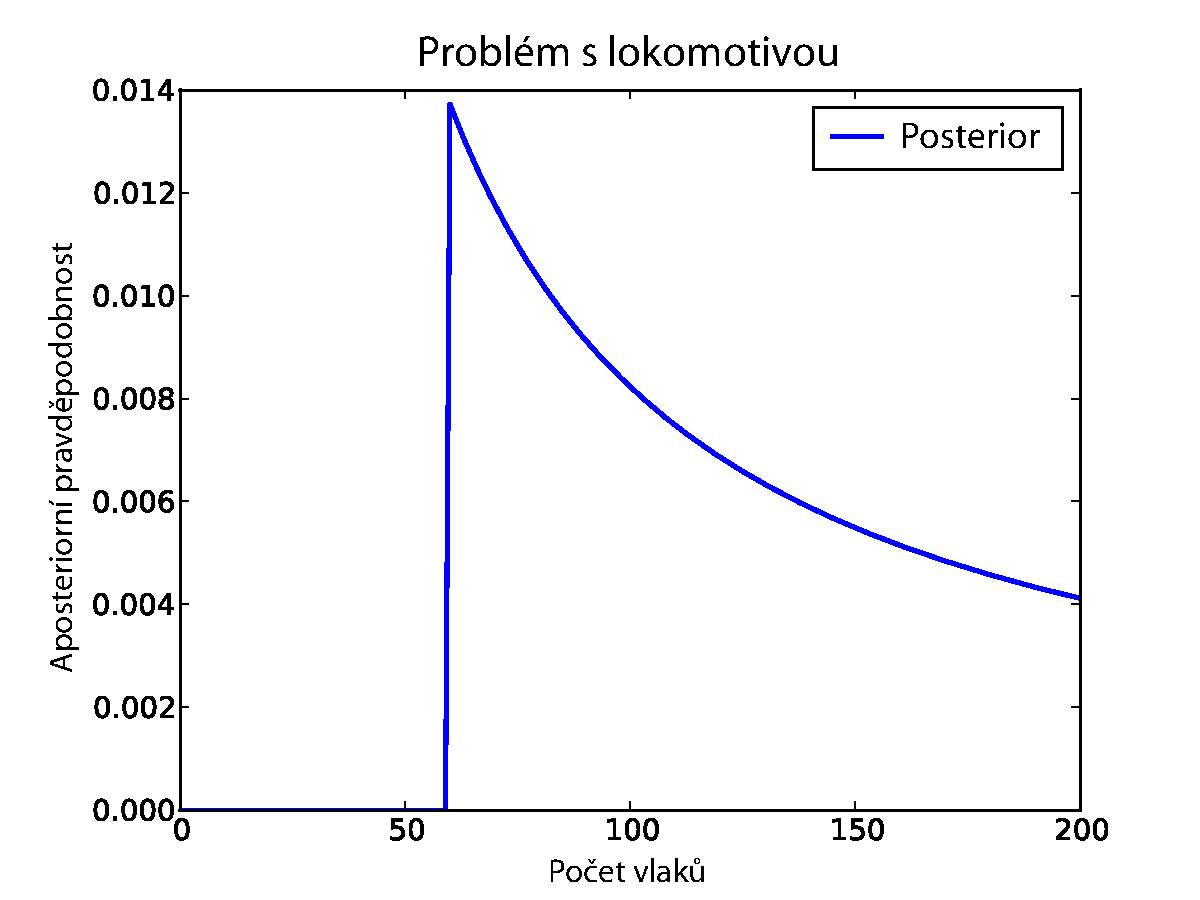
\includegraphics[height=2.5in]{figs/locomotive.pdf}}
\caption{Aposteriorní rozdělení počtu vlaků.}
\label{locomotive}
\end{figure}

Konečně pak, abychom vypočetli bayesovské aposteriorní rozdělení, vypočteme
%
\[ P(H_n \given i) = \frac{P(i \given H_n) P(H_n)}{P(i)} \]
%
Kde \HH\sub{n} je hypotéza, že existuje \n~vlaků, a \ii~je důkaz:
viděli jsme vlak \ii.  Opět \Prob(\ii|\HH\sub{n})
je 1/\n, jestliže \ii~< \n, a jinak 0.  Normalizační konstanta,
\Prob(\ii), je součet čitatelů pro každou hypotézu.
\index{bayesovský odhad}
\index{apriorní rozdělení}

Jestliže je apriorní rozdělení rovnoměrné od 1 do 200, začneme s 200
hypotézami a vypočteme pravděpodobnost každé z nich. Provedení si můžete stáhnout z:
\url{http://thinkstats.com/locomotive.py}.  Obrázek~\ref{locomotive} ukazuje, jak vypadá výsledek.
\index{{\tt locomotive.py}}
\index{rovnoměrné rozdělení}
\index{rozdělení!rovnoměrné}

90\% credible interval pro toto aposteriorní rozdělení je [63, 189], což je stále dost široký interval.
To, že jsme viděli jeden vlak, neposkytuje silný důkaz pro žádnou z hypotéz (i když vylučuje hypotézy s \n~<~\ii).
\index{credible interval}

Začneme-i s jiným apriorním rozdělením, je aposteriorní rozdělení odlišné, což pomáhá vysvětlit, proč jsou ostatní odhady tak různorodé.

Jedním ze způsobů, jak uvažovat o různých odhadech, je to, že jsou implicitně založeny na odlišných apriorních rozděleních. Jestliže existují dostatečné důkazy, které zastíní apriorní rozdělení, pak mají všechny odhady tendenci konvergovat; jinak, jako v tomto případě, neexistuje žádný odhad, který by v sobě spojoval všechny vlastnosti, které bychom potřebovali.

\begin{exercise}
Zobecněte \verb"locomotive.py", abyste se vypořádali s případem, kdy uvidíte více než jeden vlak. Změna by se měla dotknout pouze několika řádek kódu.
\index{{\tt locomotive.py}}

Zjistěte, jestli byste byli schopni zodpovědět ostatní otázky týkající se případu, kdy uvidíte více než jeden vlak. Diskusi o tomto problému a několik řešení najdete zde: \url{http://wikipedia.org/wiki/German_tank_problem}.

\end{exercise}

\section{\protect\raggedright Glosář}

\begin{description}

\item[odhadování (estimation):] Proces vyvození parametrů rozdělení ze vzorku.
\index{odhad}

\item[odhad (estimator):] Statistika používaná k odhadu parametru.
\index{odhad}

\item[střední kvadratická chyba (mean squared error):] Míra chyby odhadu.
\index{střední kvadratická chyba}
\index{MSE}

\item[maximálně věrohodný odhad (maximum likelihood estimator):] Odhad, který vypočte bodový odhad s nejvyšší věrohodností.
\index{MLE}
\index{maximálně věrohodný odhad}

\item[zkreslení (bias):] Tendence odhadu být nad nebo pod skutečnou hodnotou parametru, při zprůměrování pro opakované vzorky.
\index{zkreslený odhad}

\item[bodový odhad (point estimate):] Odhad vyjádřený jako jediná hodnota.
\index{bodový odhad}

\item[interval spolehlivosti (confidence interval):] Odhad vyjádřený jako interval s konkrétní pravděpodobností, že obsahuje skutečnou hodnotu parametru.
\index{interval spolehlivosti}
\index{interval!spolehlivosti}

\item[credible interval:] Jiný název pro bayesovský interval spolehlivosti.
\index{credible interval}
\index{interval!credible}

\item[cenzurovaná data (censored data):] Soubor dat vybraný způsobem, který systematicky vylučuje některá data.
\index{cenzurovaná data}

\end{description}


\chapter{Korelace}

\section{\protect\raggedright Standardní skóre}

V této kapitole se budeme zabývat vztahy mezi proměnnými. Například tušíme, že výška souvisí s váhou. Vyšší lidé obvykle také více váží.   {\bf Korelace} popisuje tento typ vztahu.
\index{korelace}

Měření korelace je ztíženo tím, že proměnné, které chceme porovnávat, nemusí být vyjádřeny ve stejných jednotkách. Například výška může být uvedena v centimetrech, zatímco váha v kilogramech. A i když jsou vyjádřeny ve stejných jednotkách, nejsou ze stejných rozdělení.
\index{jednotky}

Tyto problémy se běžně řeší dvěma způsoby:

\begin{enumerate}

\item Transformací všech hodnot na {\bf standardní skóre}.  Výsledkem je Pearsonův korelační koeficient.
\index{standardní skóre}
\index{Pearsonův korelační koeficient}
\index{Spearmanův korelační koeficient}
\index{koeficient!korelační}

\item Transformací všech hodnot na jejich percentilové pořadí.  Výsledkem je Spearmanův koeficient.
\index{pořadí}
\index{percentilové pořadí}

\end{enumerate}

Jestliže \X~je řada hodnot, \xsubi, můžeme provést transformaci na standardní skóre odečtením průměru a vydělením směrodatnou odchylkou:
z\sub{i}~=~(x\sub{i}~\minus~\mymu) / \mysigma.
\index{průměr}
\index{směrodatná odchylka}

Čitatel představuje odchylku: vzdálenost od průměru.  Vydělení směrodatnou odchylkou
\mysigma~{\bf normalizuje} tuto odchylku, takže hodnoty \Z~jsou bezrozměrné
(bez jednotek) a jejich rozdělení má průměr 0 a rozptyl 1.
\index{normalizovat}
\index{odchylka}
\index{normální rozdělení}
\index{rozdělení!normální}
\index{Gaussovo rozdělení}
\index{rozdělení!Gaussovo}

Má-li \X~normální rozdělení, pak ho má také \Z; jestliže je však \X~sešikmené nebo obsahuje odlehlé hodnoty, pak totéž platí i pro \Z.  V těchto případech je robustnější použít percentilová pořadí.
Obsahuje-li \R~percentilová pořadí hodnot v \X, je rozdělení \R~stejnoměrné mezi 0 a 100,
bez ohledu na rozdělení \X.
\index{rovnoměrné rozdělení}
\index{rozdělení!rovnoměrné}
\index{robustní}

\section{\protect\raggedright Kovariance}
\index{kovariance}
\index{odchylka}

{\bf Kovariance} vyjadřuje míru tendence dvou proměnných ke společné variabilitě. (Lze použít u proměnných, které mají stejné jednotky. Kovariance standardizovaná na variabilitu dat je pak korelací.)
Máme-li dvě řady, \X~a \Y, jejich odchylky od průměru jsou

\Eqn{ \dd\x\sub{i} = \x\sub{i}~\minus~\mymu\sub{X} }

\Eqn{ \dd\y\sub{i} = \y\sub{i}~\minus~\mymu\sub{Y} }

kde \mymu \sub{X} je průměr \X~a \mymu \sub{Y} průměr \Y.
Jestliže se \X~a \Y~mění společně, jejich odchylky mají tendenci ke stejnému znaménku.

Jestliže je společně vynásobíme, součin je kladný, mají-li odchylky stejné znaménko, a záporný, mají-li opačné znaménko. Sečtením součinů tak získáme míru jejich tendence k tomu, aby se měnili společně.

Kovariance je průměr těchto součinů:
%
\[ Cov(X,Y) = \frac{1}{n} \sum dx_i dy_i \]
%
kde \n~je délka příslušných dvou řad (musí být stejně dlouhé).

Kovariance je užitečná u některých výpočtů, ale zřídkakdy se uvádí jako souhrnná statistická charakteristika, protože je obtížné ji interpretovat. Mimo jiné jsou její jednotky součinem jednotek \X~a\Y.  Takže kovariance váhy a výšky by mohla být vyjádřena v jednotkách kilogram-metr, což nemá příliš velký význam.

\begin{exercise}
Napište funkci s názvem {\tt Cov}, která přijme dva seznamy a vypočítá jejich kovarianci. K otestování vaší funkce vypočítejte kovarianci seznamu se sebou samým a ověřte, že
Cov(\X, \X)~=~Var(\X).

Řešení si můžete stáhnout z
\url{http://thinkstats.com/correlation.py}.
\index{{\tt correlation.py}}

\end{exercise}


\section{\protect\raggedright Korelace}
\index{korelace}
\index{standardní skóre}

Jedním možným řešením je vydělit odchylky směrodatnou odchylkou \mysigma,
čímž získáme standardní skóre, a vypočíst součin standardních skóre:
%
\[ p_i = \frac{(x_i - \mu_X)}{\sigma_X} \frac{(y_i - \mu_Y)}{\sigma_Y} \]
%
Průměr těchto součinů je
%
\[ \rho = \frac{1}{n} \sum p_i \]
%

Nebo můžeme přepsat \myrho~vytknutím \mysigma \sub{X} a
\mysigma \sub{Y}:
%
\[ \rho = \frac{Cov(X,Y)}{\sigma_X \sigma_Y} \]
%

Tato hodnota se označuje jako {\bf Pearsonova korelace} a je pojmenována po Karlu Pearsonovi,
významném statistikovi, který se podílel na formování této vědní disciplíny.  Tento ukazatel se snadno počítá a snadno interpretuje. Protože standardní skóre jsou bezrozměrná, stejně tak je tomu i v případě \myrho.
\index{Pearson, Karl}
\index{Pearsonův korelační koeficient}
\index{koeficient!korelační}

Pearsonova korelace se vždy pohybuje mezi -1 a +1 (včetně obou).
Její velikost ukazuje na sílu korelace. Jestliže \myrho~=~1, proměnné dokonale korelují, což znamená, že pokud znáte jednu z nich, můžete dokonale předpovědět druhou z nich. Totéž platí, jestliže \myrho~=~\minus1.  To znamená, že mezi proměnnými existuje negativní (nepřímá) korelace, avšak pro účely predikce je negativní korelace právě tak dobrá, jako pozitivní (přímá) korelace.
\index{predikce}

Většina korelací v reálném světě není absolutní, ale přesto je tento vztah užitečný. Například jestliže znáte něčí výšku, mohli byste odhadnout váhu daného člověka. Možná se netrefíte úplně přesně, ale pořád bude váš odhad lepší, než kdybyste vůbec neznali jeho výšku. Pearsonova korelace je mírou toho, o kolik lepší je takový odhad.

Jestliže tedy platí \myrho~=~0, znamená to, že mezi proměnnými neexistuje žádný vztah? Bohužel nikoliv. Pearsonova korelace měří pouze {\em lineární} vztahy. Existuje-li mezi proměnnými nelineární vztah, \myrho~nevyjadřuje plně sílu dané závislosti.
\index{lineární vztah}

\begin{figure}
% descriptive.py
\centerline{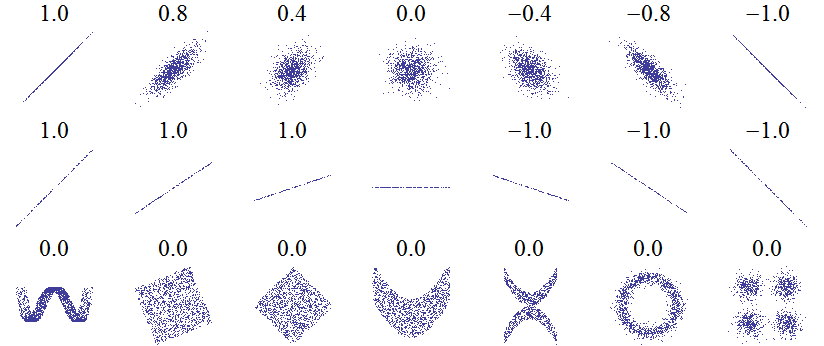
\includegraphics[height=2.5in]{figs/Correlation_examples.png}}
\caption{Příklady souborů dat se škálou korelací.}
\label{corr_examples}
\end{figure}

Obrázek~\ref{corr_examples} je převzatý z
\url{http://wikipedia.org/wiki/Correlation_and_dependence}.  Ukazuje bodové grafy a korelační koeficienty pro několik pečlivě sestavených souborů dat.
\index{koeficient!korelační}
\index{bodový graf}
\index{graf!bodový}

Horní řada ukazuje lineární vztahy se škálou korelací. Na základě této řady si můžete vytvořit představu o tom, jak vypadají různé hodnoty \myrho. Druhá řada ukazuje dokonalé korelace s různými sklony, což dokládá, že korelace nemá žádný vztah ke sklonu (o odhadování sklonu se záhy zmíním). Třetí řada ukazuje proměnné, které jsou evidentně vzájemně provázané, ale protože jejich vztah je nelineární, korelační koeficient se rovná 0.

Ponaučení, které z toho plyne, je, že byste se měli vždy podívat na bodový graf vašich dat před tím, než slepě vypočítáte korelační koeficient.
\index{korelační koeficient}
\index{koeficient!korelační}

\begin{exercise}
Napište funkci nazvanou {\tt Corr}, která přijme dva seznamy a vypočítá jejich korelaci. Nápověda: Použijte {\tt thinkstats.Var} a
funkci {\tt Cov}, kterou jste vytvořili v předešlém cvičení.
\index{rozptyl}
\index{kovariance}

K otestování vaší funkce vypočtěte kovarianci seznamu se sebou samým a ověřte, že Corr(\X, \X) je 1.  Řešení si můžete stáhnout z \url{http://thinkstats.com/correlation.py}.
\index{{\tt correlation.py}}

\end{exercise}


\section{\protect\raggedright Vytváření bodových grafů v pyplot}
\index{bodový graf}
\index{graf!bodový}
\index{pyplot}

\begin{figure}
% brfss_corr.py
\centerline{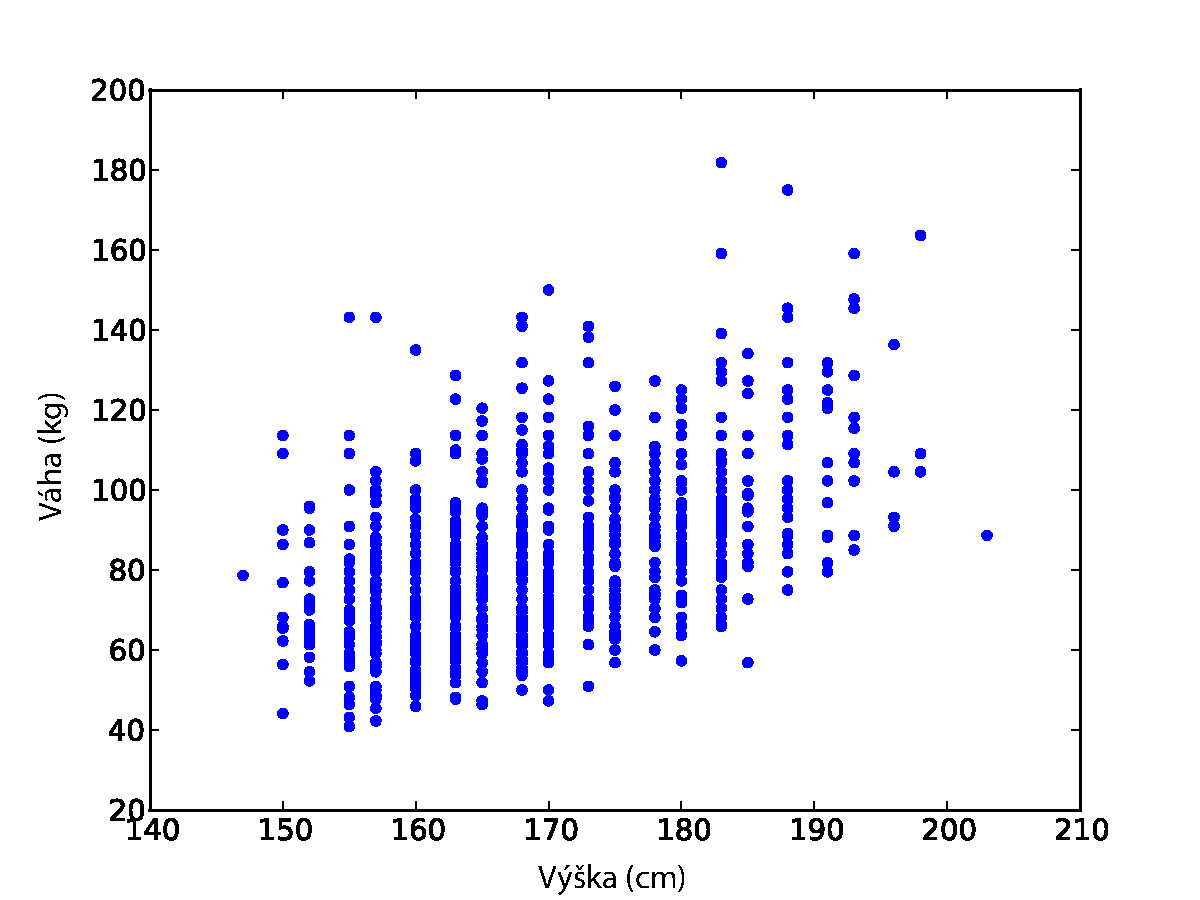
\includegraphics[height=2.5in]{figs/scatter1.pdf}}
\caption{Jednoduchý bodový graf znázorňující vztah mezi váhou a výškou u respondentů v rámci
BRFSS.}
\label{scatterplot1}
\end{figure}

\begin{figure}
% brfss_corr.py
\centerline{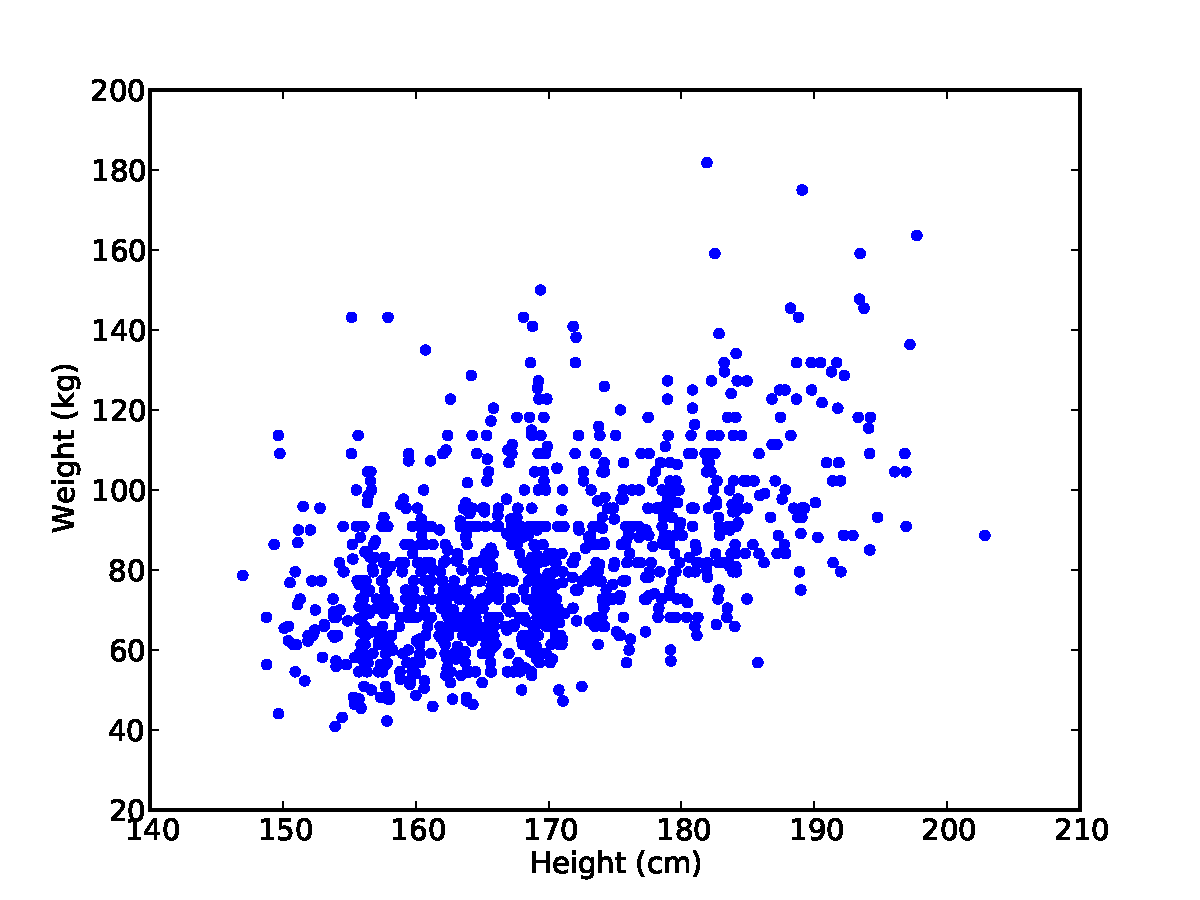
\includegraphics[height=2.5in]{figs/scatter2.pdf}}
\caption{Bodový graf s daty, na která byla aplikována metoda jitter.}
\label{scatterplot2}
\end{figure}

\begin{figure}
% brfss_corr.py
\centerline{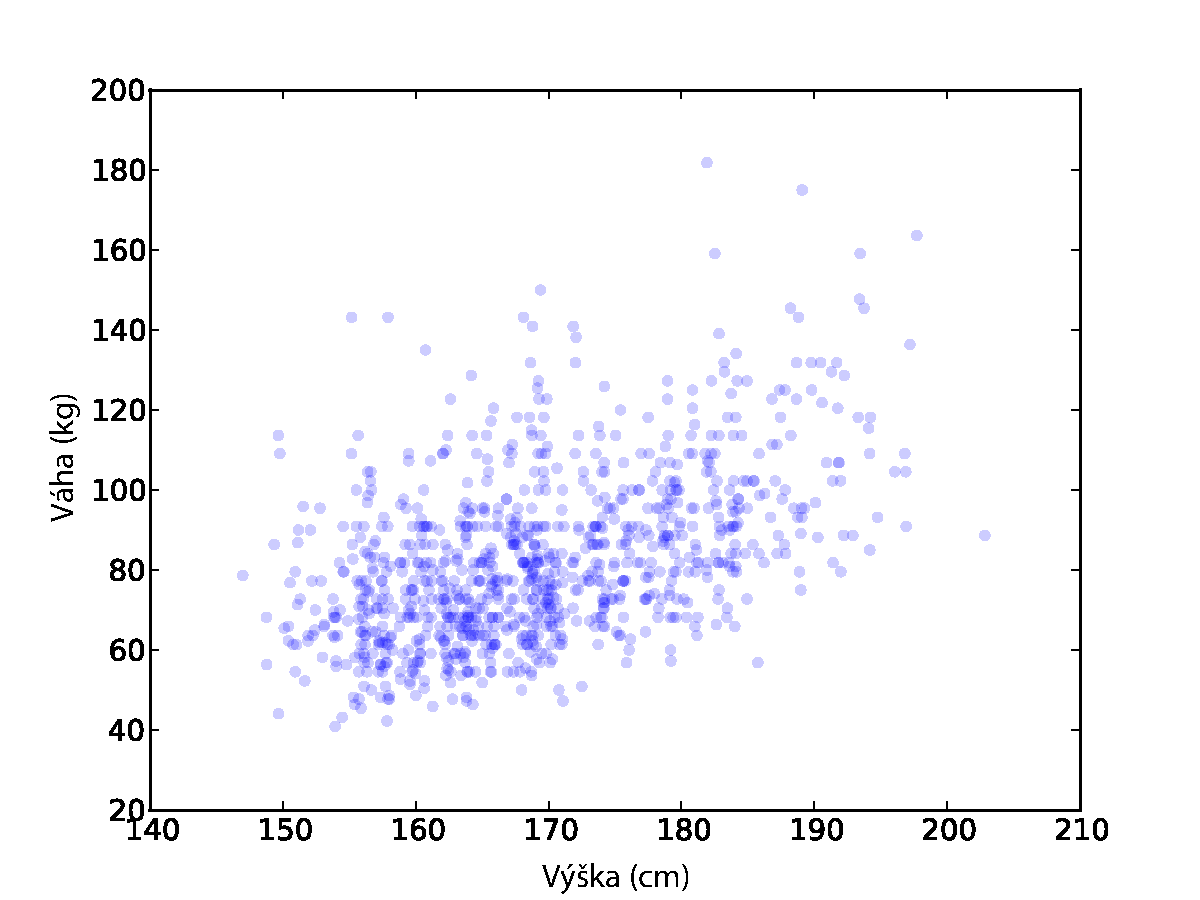
\includegraphics[height=2.5in]{figs/scatter3.pdf}}
\caption{Bodový graf, ve kterém byla uplatněna metoda jitter a transparency.}
\label{scatterplot3}
\end{figure}

\begin{figure}
% brfss_corr.py
\centerline{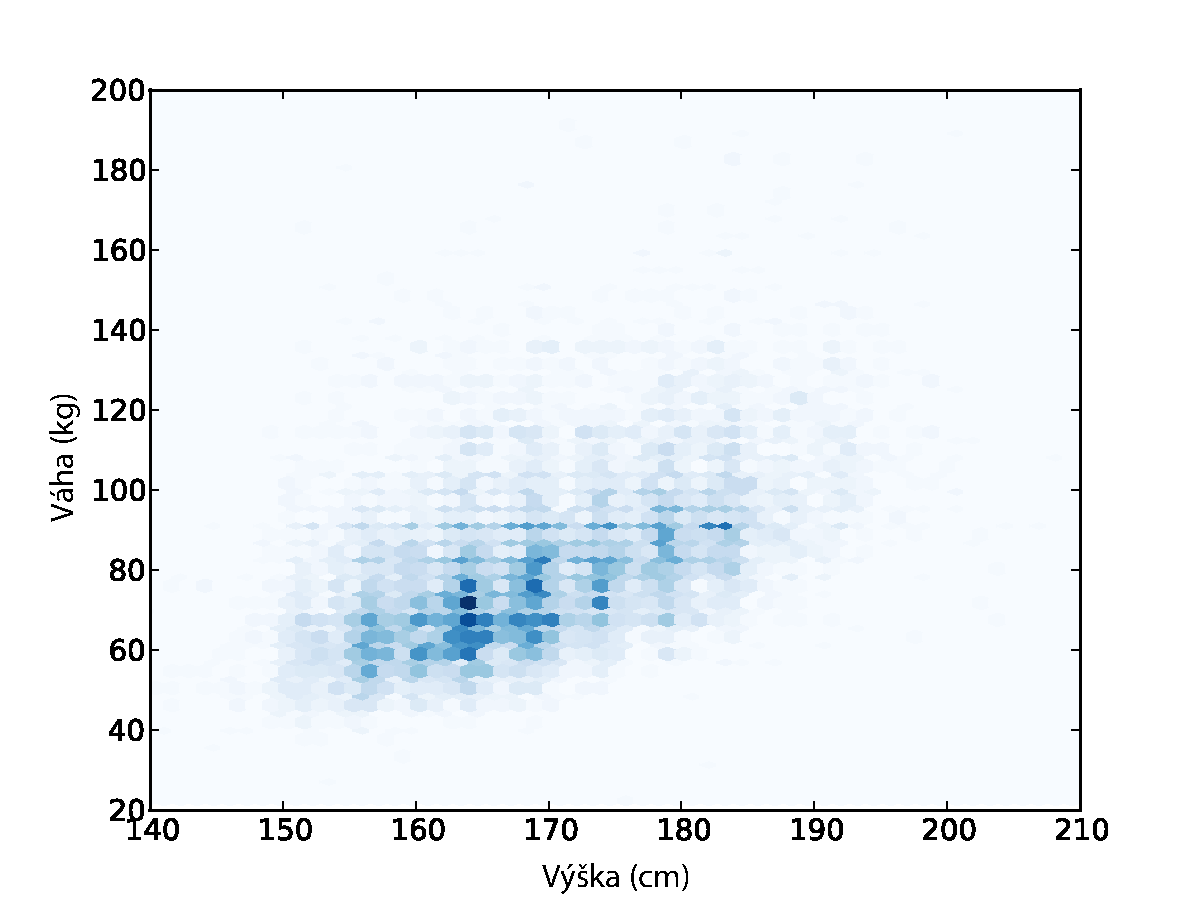
\includegraphics[height=2.5in]{figs/scatter4.pdf}}
\caption{Bodový graf s daty rozdělenými do tříd za použití {\tt pyplot.hexbin}.}
\label{scatterplot4}
\end{figure}
\index{Systém sledování rizikových faktorů chování -- Behavioral Risk Factor Surveillance System}
\index{BRFSS}

Nejjednodušší způsob, jak prověřit vztah mezi dvěma proměnnými, je sestavit bodový graf. Vytvoření dobrého bodového grafu ale není vždy snadné. Jako příklad vytvořím graf zobrazující vztah mezi váhou a výškou u respondentů z šetření BRFSS (viz Oddíl~\ref{lognormal}).  {\tt pyplot} obsahuje funkci nazvanou
{\tt scatter}, která vytváří bodové grafy:
%
\begin{verbatim}
import matplotlib.pyplot as pyplot
pyplot.scatter(heights, weights)
\end{verbatim}

Na Obrázku~\ref{scatterplot1} je vidět výsledek.  Není překvapením, že ukazuje na pozitivní korelaci -- vyšší lidé jsou obvykle také těžší. Není to ale zrovna nejlepší způsob zobrazení dat, protože data vytváří sloupcové shluky. Problém spočívá v tom, že údaje o hmotnosti byly zaokrouhleny na nejbližší palec, pak převedeny na centimetry a znovu zaokrouhleny. V průběhu tohoto procesu se některé informace ztratily.
\index{výška}
\index{váha}
\index{jitter}

Tyto informace už nedostaneme zpátky, ale dopad na bodový graf můžeme minimalizovat pomocí metody {\bf jitter}, aplikované na data. Podstatou této metody je dodání náhodného šumu, abychom vyvážili vliv zaokrouhlení.  Protože byly naměřené hodnoty zaokrouhleny na nejbližší palec, mohou být nepřesné až o 0,5 palce nebo 1,3 cm. Proto jsem dodal stejnoměrný šum v rozpětí \minus1,3 až 1,3:
\index{rovnoměrné rozdělení}
\index{rozdělení!rovnoměrné}
\index{šum}
%
\begin{verbatim}
jitter = 1.3
heights = [h + random.uniform(-jitter, jitter) for h in heights]
\end{verbatim}

Na Obrázku~\ref{scatterplot2} je zobrazen výsledek. Na základě použití metody jitter je tvar vztahu zřejmější. Obecně byste měli k uplatnění metody jitter přistoupit pouze pro účely vizualizace a datům upraveným pomocí metody jitter se vyhnout, pokud je chcete analyzovat.

Dokonce ani když použijete metodu jitter, není to ten nejlepší způsob zobrazení dat. V grafu je spousta bodů, které se překrývají, což vede k tomu, že data v hustě pokrytých částech jsou skrytá a naopak nepřiměřenou pozornost strhávají odlehlé hodnoty.
\index{odlehlá hodnota}

Toto můžeme vyřešit pomocí parametru {\tt alpha}, díky němuž se stanou body částečně transparentními:
%
\begin{verbatim}
pyplot.scatter(heights, weights, alpha=0.2)
\end{verbatim}
%
Na Obrázku~\ref{scatterplot3} je zobrazen výsledek.  Překrývající se datové body vypadají tmavší, takže tmavost je proporcionální k hustotě. V této verzi grafu je patrný pozorovaný artefakt -- horizontální přímka poblíž 90 kg nebo 200 liber. Vzhledem k tomu, že data vychází z údajů v librách, které o sobě poskytli respondenti sami, jako nejpravděpodobnější se nabízí vysvětlení, že některé hodnoty byly zaokrouhleny (dost možná směrem dolů).

Použití metody transparency funguje dobře u nepříliš velkých datových souborů, ale na tomto obrázku je zobrazeno pouze prvních 1000 záznamů v rámci BRFSS, z celkových 414509.
\index{hexbin graf}
\index{graf!hexbin}

Pro větší soubory dat je jednou z možností hexbin graf, který rozdělí graf do hexagonálních tříd a každou třídu vybarví podle toho, kolik datových bodů do ní patří. {\tt pyplot} obsahuje funkci s názvem {\tt hexbin}:
%
\begin{verbatim}
pyplot.hexbin(heights, weights, cmap=matplotlib.cm.Blues)
\end{verbatim}
%
Obrázek~\ref{scatterplot4} ukazuje výsledek za použití mapy modré barvy.
Předností hexbin grafu je, že dobře znázorňuje tvar vztahu a je efektivní při práci s velkými soubory dat. Nevýhodou je, že odlehlé hodnoty se stávají neviditelnými.
\index{barevná mapa}
\index{stupnice šedi}

Ponaučení, které z toho plyne, je, že není snadné vytvořit bodový graf, který není potenciálně zavádějící. Kód pro uvedené obrázky si můžete stáhnout z
\url{http://thinkstats.com/brfss_scatter.py}.
\index{{\tt brfss\_scatter.py}}

\section{\protect\raggedright Spearmanova pořadová korelace}

Pearsonova korelace funguje dobře, jestliže mezi proměnnými existuje lineární vztah a jestliže se jedná o proměnné s přibližně normálním rozdělením. Není ale robustní, jsou-li přítomny odlehlé hodnoty.
\index{Pearsonův korelační koeficient}
\index{Spearmanův korelační koeficient}
\index{koeficient!korelační}
\index{normální rozdělení}
\index{rozdělení!normální}
\index{Gaussovo rozdělení}
\index{rozdělení!Gaussovo}

Toto zjištění dobře dokládá Anscombeho kvartet, který obsahuje čtyři soubory dat se stejnou korelací. V jednom souboru existuje lineární vztah s náhodným šumem, druhý představuje nelineární vztah, další je dokonalý vztah s odlehlou hodnotou a u posledního neexistuje žádný vztah kromě artefaktu způsobeného odlehlou hodnotou. O tomto kvartetu si můžete přečíst více na
\url{http://wikipedia.org/wiki/Anscombe's_quartet}.
\index{Anscombeho kvartet}

Spearmanova pořadová korelace představuje alternativu, která zmírňuje působení odlehlých hodnot a sešikmených rozdělení. K výpočtu Spearmanovy korelace musíme spočítat {\bf pořadí} každé hodnoty, které je jejím indexem v rámci setříděného vzorku. Například ve vzorku \{7, 1, 2, 5\} má hodnota 5 pořadí 3, protože pokud jednotlivé členy seřadíme, pak se nachází na třetím místě. Pak spočítáme Pearsonovu korelaci pro pořadí.

Alternativou ke Spearmanově korelaci je použít transformaci, která data více přiblíží normálnímu rozdělení, a pak vypočítat Pearsonovu korelaci pro transformovaná data. Například mají-li data přibližně logaritmicko-normální rozdělení, můžete vzít logaritmus každé hodnoty a vypočítat korelaci logaritmů.
\index{logaritmicko-normální rozdělení}
\index{rozdělení!logaritmicko-normální}

\begin{exercise}
Napište funkci, která přijme řadu a vrátí seznam uvádějící pořadí jednotlivých členů. Například pro řadu \{7, 1, 2, 5\} bude výsledek \{ 4, 1, 2, 3\}.

Vyskytuje-li se stejná hodnota víckrát, striktně korektní řešení by bylo přiřadit každé z nich průměr jejich pořadí. Pokud to však budeme ignorovat a pořadí jim přiřadíme v náhodném sledu, chyba obvykle bývá jen malá.

Napište funkci, která přijme dvě řady (o stejné délce) a vypočte jejich Spearmanův pořadový koeficient. Řešení si můžete stáhnout z \url{http://thinkstats.com/correlation.py}.
\index{{\tt correlation.py}}
\index{Spearmanův korelační koeficient}
\index{koeficient!korelační}

\end{exercise}


\begin{exercise}
Stáhněte si \url{http://thinkstats.com/brfss.py} a
\url{http://thinkstats.com/brfss_scatter.py}.  Spusťte je a ujistěte se, že jste schopni číst data z BRFSS a generovat bodové grafy.
\index{Systém sledování rizikových faktorů chování -- Behavioral Risk Factor Surveillance System}
\index{BRFSS}
\index{{\tt brfss.py}}
\index{{\tt brfss\_scatter.py}}

Porovnáte-li bodové grafy s Obrázkem~\ref{corr_examples}, jakou hodnotu Pearsonovy korelace očekáváte? A jaká hodnota vám vyšla?
\index{hmotnost!dospělých}
\index{hmotnost dospělých}
\index{logaritmicko-normální rozdělení}
\index{rozdělení!logaritmicko-normální}
\index{odlehlá hodnota}

Protože rozdělení váhy dospělých je logaritmicko-normální, vyskytují se v něm odlehlé hodnoty, které ovlivňují korelaci. Pokuste se graficky znázornit vztah log(váha) versus výška a vypočíst Pearsonovu korelaci pro transformovanou proměnnou.

Nakonec pak vypočtěte Spearmanovu pořadovou korelaci pro váhu a výšku. Který koeficient je podle vás nejlepším ukazatelem síly tohoto vztahu? Řešení si můžete stáhnout zde:
\url{http://thinkstats.com/brfss_corr.py}.
\index{{\tt brfss\_corr.py}}

\end{exercise}


\section{\protect\raggedright Metoda nejmenších čtverců}

Korelační koeficienty měří sílu a znaménko vztahu, ale ne sklon. Pro odhad sklonu existuje několik možností. Nejčastěji se používá {\bf lineární regrese metodou nejmenších čtverců}.  ``Lineární regrese'' je proložení dat přímkou, která slouží k modelování vztahu mezi proměnnými. Metoda ``nejmenších čtverců'' je metoda, která minimalizuje střední kvadratickou chybu (MSE) mezi přímkou a daty\footnote{Viz
  \url{http://wikipedia.org/wiki/Simple_linear_regression}.}.
\index{metoda nejmenších čtverců}
\index{lineární regrese metodou nejmenších čtverců}
\index{koeficient!korelační}
\index{lineární regrese}

Předpokládejme, že máme řadu bodů \Y, kterou chceme vyjádřit jako funkci jiné řady
\X. Jestliže mezi \X~a \Y~ existuje lineární vztah s konstantou \myinter~a sklonem \myslope, očekáváme, že každé \y\sub{i} bude přibližně \myinter~+ \myslope~\x\sub{i}.
\index{reziduum}

Pokud se ale nejedná o dokonalou korelaci, je tato predikce pouze přibližná. Odchylka, neboli {\bf reziduum} je

\Eqn{ \myeps\sub{i}~=~(\myinter~+~\myslope \x\sub{i})~\minus~\y\sub{i} }

Reziduum může být způsobeno náhodnými faktory, jako například chybou měření, nebo nenáhodnými faktory, které jsou neznámé. Například pokoušíme-li se predikovat váhu jako funkci výšky, neznámými faktory mohou být způsob stravování, cvičení a tělesný typ.
\index{sklon}
\index{konstanta}

Jestliže použijeme nesprávné parametry \myinter~a \myslope, rezidua budou větší, a tak intuitivně dává smysl, že by požadované parametry měly být takové, které minimalizují rezidua.


Jako obvykle bychom mohli minimalizovat absolutní hodnotu reziduí, nebo jejich druhých mocnin, nebo třetích mocnin atd. Nejběžnější volbou je minimalizovat součet kvadratických reziduí
%
\[ \min_{\inter, \slope} \sum \eps_i^2 \]
%
Proč?  Existují pro to tři dobré a jeden špatný důvod:

\begin{itemize}

\item Umocnění na druhou má zřejmý efekt -- s kladnými i zápornými rezidui je nakládáno stejně, což většinou chceme.

\item Umocněním na druhou získávají větší rezidua na váze, avšak ne natolik, aby největší reziduum vždy dominovalo.

\item Jestliže jsou rezidua nezávislá na \x, náhodná a mají normální rozdělení s
  \mymu~=~0 a konstantní (ale neznámou) \mysigma, pak je metoda nejmenších čtverců také maximálně věrohodným odhadem \myinter~a \myslope.\footnote{Viz Press et al., {\em Numerical Recipes in C},
    Chapter 15 at \url{http://www.nrbook.com/a/bookcpdf/c15-1.pdf}.}
\index{MLE}
\index{maximálně věrohodný odhad}

\item Hodnoty $\hat{\inter}$ a $\hat{\slope}$, které minimalizují kvadratická rezidua, mohou být efektivně vypočteny.

\end{itemize}

Poslední důvod byl opodstatněný ve chvíli, kdy byla výpočetní účinnost důležitější než volba nejvhodnější metody pro řešený problém. To už ale neplatí, a tak stojí za to zvážit, jestli kvadratická rezidua jsou opravdu tím, co je potřeba minimalizovat.
\index{výpočet}

Jestliže například používáte hodnoty \X~k predikování hodnot \Y,
příliš vysoký odhad by mohl být lepší (nebo horší), než příliš nízký odhad. V takovém případě by se vám mohlo hodit vypočíst nákladovou funkci, cost(\myeps\sub{i}), a minimalizovat celkové náklady.
\index{nákladová funkce}

Nicméně výpočet metodou nejmenších čtverců je rychlý, snadný a často také dostatečně dobrý. Podívejme se tedy na postup:

\begin{enumerate}

\item Vypočtěte výběrové průměry, \myxbar~a \myybar, rozptyl \X~a kovarianci \X~a \Y.

\item Odhadovaný sklon je
%
\[ \hat{\slope} = \frac{Cov(X,Y)}{Var(X)} \]
%
\item A konstanta je
%
\[ \hat{\inter} = \ybar - \hat{\slope} \xbar \]
%
\end{enumerate}

Pokud vás zajímá, jak je toto odvozeno, přečtěte si \url{http://wikipedia.org/wiki/Numerical_methods_for_linear_least_squares}.


\begin{exercise}
Napište funkci nazvanou {\tt LeastSquares}, která přijme \X~a \Y~a vypočítá
 $\hat{\inter}$ a $\hat{\slope}$.  Řešení si můžete stáhnout zde:
\url{http://thinkstats.com/correlation.py}.  \index{{\tt
    correlation.py}}

\end{exercise}

\begin{exercise}
Opět za použití dat z šetření BRFSS vypočtěte lineární regresi metodou nejmenších čtverců pro log(váha) versus výška. Řešení si můžete stáhnout z \url{http://thinkstats.com/brfss_corr.py}.
\index{Systém sledování rizikových faktorů chování -- Behavioral Risk Factor Surveillance System}
\index{BRFSS}
\index{{\tt brfss\_corr.py}}

\end{exercise}


\begin{exercise}
Rozdělení rychlosti větru na konkrétním místě určuje hustotu větrné energie, což představuje horní hranici průměrného množství energie, kterou je větrná turbína na daném místě schopna vygenerovat. Podle některých zdrojů k modelování empirických rozdělení rychlosti větru dobře slouží Weilbullovo rozdělení (viz \url{http://wikipedia.org/wiki/Wind_power#Distribution_of_wind_speed}).
\index{rychlost větru}
\index{hustota větrné energie}
\index{turbína}
\index{Weibullovo rozdělení}
\index{rozdělení!Weibullovo}

Pro posouzení toho, zda je konkrétní místo vhodné pro umístění větrné turbíny, můžete na místě instalovat anemometr a měřit po určitou dobu rychlost větru. Je však obtížné změřit přesně chvost rozdělení rychlosti větru, protože, jak vyplývá z povahy věci, jevy na chvostu nenastávají příliš často.
\index{chvost}

Jedním ze způsobů, jak si s tímto problémem poradit, je použít měření k odhadu parametrů Weilbullova rozdělení a pak integrovat přes spojitou PDF za účelem výpočtu hustoty větrné energie.
\index{PDF}

K odhadu parametrů Weilbullova rozdělení můžeme použít transformaci ze Cvičení ~\ref{weibull} a pak použít lineární regresi k nalezení sklonu a konstanty transformovaných dat.

Napište funkci, která přijme vzorek z Weilbullova rozdělení a odhadne jeho parametry.

Nyní napište funkci, která přijme parametry Weilbullova rozdělení rychlosti větru a vypočte průměrnou hustotu větrné energie (zřejmě bude nutné provést nějaký průzkum, abyste se orientovali v této části).

\end{exercise}


\section{\protect\raggedright Dobrá shoda}
\index{dobrá shoda}
\index{shoda, dobrá}

Jestliže jsme nalezli shodu mezi lineárním modelem a daty, mohlo by nás zajímat, o jak dobrou shodu se jedná.  To ale záleží na tom, jakému má sloužit účelu. Jedním možným způsobem hodnocení modelu je jeho predikční síla.

V kontextu predikce se veličina, kterou se pokoušíme odhadnout, nazývá {\bf závisle proměnná} a veličina, kterou používáme k odhadu, se nazývá {\bf nezávisle proměnná}.
\index{závisle proměnná}
\index{nezávisle proměnná}
\index{koeficient!determinační}

Abychom změřili prediktivní sílu modelu, můžeme vypočítat {\bf
  determinační koeficient}, běžněji známý jako ``R na druhou'':
%
\[ R^2 = 1 - \frac{Var(\eps)}{Var(Y)}\]
%
K pochopení toho, co znamená \R\super{2}, uvažujte (znovu) situaci, kdy se pokoušíte odhadnout váhu nějakého člověka. Pokud byste o dané osobě nevěděli vůbec nic, nejlepší strategií by bylo odhadnout \myybar; v tom případě by střední kvadratická chyba (MSE) vašich odhadů byla Var(\Y):
%
\[ MSE = \frac{1}{n} \sum (\ybar - y_i)^2 = Var(Y) \]
%
Kdybych vám ale řekl výšku daného člověka, odhadli byste $\hat{\inter} +
\hat{\slope}$ \x\sub{i}; v tom případě by vaše MSE byla Var(\myeps).
%
\[ MSE =
\frac{1}{n} \sum (\hat{\inter} + \hat{\slope} x_i - y_i)^2 =
Var(\eps) \]
%
Výraz Var(\myeps)/Var(\Y) tedy představuje poměr střední kvadratické chyby s nezávisle proměnnou a bez ní, což je podíl variability, kterou model nechává bez vysvětlení. Komplement, \R\super{2},
je pak podíl variability, kterou model vysvětluje.
\index{variabilita}

Jestliže v modelu vychází, že \R\super{2}~=~0,64, mohli byste říci, že model vysvětluje
64 \% variability, nebo pokud byste chtěli být přesnější, že redukuje střední kvadratickou chybu (MSE) vašich predikcí o 64 \%.

V kontextu modelu lineární regrese metodou nejmenších čtverců se ukazuje, že mezi determinačním koeficientem a Pearsonovým korelačním koeficientem \myrho~existuje jednoduchý vztah:

\Eqn{ \R\super{2} = \myrho\super{2} }

Viz \url{http://wikipedia.org/wiki/Howzzat}!
\index{howzzat}

\begin{exercise}
Wechslerova škála inteligence dospělých (WAIS) slouží k měření inteligence. Skóre jsou kalibrována tak, že průměr a směrodatná odchylka v obecné populaci jsou 100 a 15.
\index{škála inteligence dospělých}
\index{WAIS}
\index{IQ}
\index{inteligence}

Předpokládejme, že chcete předpovědět něčí WAIS skóre na základě skóre, kterého daný člověk dosáhl ve standardizovaném testu SAT. Podle jedné studie existuje mezi celkovým SAT skóre a WAIS skóre Pearsonova korelace rovná
0,72.

Pokud byste váš prediktor aplikovali na velký vzorek, jakou průměrnou kvadratickou chybu (MSE) vašich predikcí byste očekávali?

Nápověda: Jaká je MSE, jestliže budete vždy odhadovat 100?
\end{exercise}


\begin{exercise}
Napište funkci s názvem {\tt Residuals}, která přijme \X, \Y, $\hat{\inter}$
a $\hat{\slope}$ a vrátí seznam \myeps\sub{i}.
\index{reziduum}

Napište funkci nazvanou {\tt CoefDetermination}, která přijme
\myeps\sub{i}~a \Y~a vrátí \R\super{2}.  K otestování vašich funkcí, ověřte, že {\R\super{2}~=~\myrho\super{2}}.  Řešení si můžete stáhnout z \url{http://thinkstats.com/correlation.py}.
\index{{\tt correlation.py}}

\end{exercise}

\begin{exercise}
Za použití dat o výšce a váze z šetření BRFSS (ještě jednou)
vypočtěte $\hat{\inter}$, $\hat{\slope}$ a \R\super{2}.  Kdybyste se pokoušeli odhadnout něčí váhu, jak moc by vám pomohlo, pokud byste znali výšku dané osoby?
Řešení si můžete stáhnout z
\url{http://thinkstats.com/brfss_corr.py}.
\index{Systém sledování rizikových faktorů chování -- Behavioral Risk Factor Surveillance System}
\index{BRFSS}
\index{{\tt brfss\_corr.py}}

\end{exercise}


\section{\protect\raggedright Korelace a kauzalita}
\index{korelace}
\index{kauzalita}
\index{xkcd}
\index{komiks}
\index{Munroe, Randall}

Webový komiks {\tt xkcd} poukazuje na to, jak obtížné je vyvodit příčinný vztah:

\begin{figure}
\centerline{
\includegraphics[width=4.0in]{figs/correlation.png}}
\caption{Převzato z {\tt xkcd.com} autora Randalla Munroa.}
\end{figure}

Obecně můžeme říci, že existence vztahu mezi dvěma proměnnými nevypovídá nic o tom, zda jedna způsobuje druhou, nebo naopak, nebo jestli obě způsobuje něco úplně jiného.

Toto pravidlo se dá shrnout větou ``Korelace neimplikuje kauzalitu'', která je natolik obsažná, že má svoji vlastní stránku na Wikipedii: \url{http://wikipedia.org/wiki/Correlation_does_not_imply_causation}.

Takže co můžete udělat, abyste získali důkaz o kauzalitě?

\begin{enumerate}

\item Využijte čas.  Jestliže A předchází B, pak A může způsobovat B, ale ne naopak (alespoň v souladu s obecně přijímaným chápáním kauzality). Pořadí jevů nám může pomoci vyvodit směr kauzality, ale nevylučuje možnost, že jak A, tak B je způsobeno něčím jiným.

\item Využijte nahodilosti.  Jestliže rozdělíte velkou populaci náhodně do dvou skupin a spočítáte průměry téměř jakékoliv proměnné, očekáváte, že rozdíl bude malý. Toto je důsledek centrální limitní věty (takže podléhá stejným požadavkům).

Jestliže jsou skupiny téměř identické ve všech proměnných až na jednu, můžete eliminovat nepravé vztahy.
\index{nepravý vztah}

  Toto funguje, i pokud nevíte, které jsou relevantní proměnné. Ale funguje to ještě lépe, pokud to víte, protože pak můžete zkontrolovat, že dané skupiny jsou identické.


\end{enumerate}

Těmito myšlenkami je motivován {\bf randomizovaný kontrolovaný test}, ve kterém jsou subjekty náhodně rozřazeny do dvou (nebo více) skupin: {\bf experimentální} skupiny, která je podrobena nějaké intervenci, jako například podání nového léku, a {\bf kontrolní skupiny}, která není podrobena žádné intervenci, nebo dostává jinou léčbu, jejíž účinky jsou známé.
\index{randomizovaný kontrolovaný test}
\index{kontrolovaný test}
\index{experimentální skupina}
\index{kontrolní skupina}
\index{lék}

Randomizovaný kontrolovaný test je nejspolehlivějším způsobem, jak demonstrovat příčinný vztah, a tvoří také základnu vědecky podložené medicíny (viz \url{http://wikipedia.org/wiki/Randomized_controlled_trial}).

Bohužel kontrolované testy jsou možné pouze v laboratorních vědách, medicíně a několika dalších disciplínách. V sociálních vědách jsou kontrolované experimenty vzácné, obvykle proto, že je nemožné je provést nebo jsou neetické.

Jednou z alternativ je hledání {\bf přirozeného experimentu}, kdy jsou různé formy
``léčby'' aplikovány na skupiny, které jsou jinak podobné. Přirozené experimenty s sebou nesou nebezpečí spočívající ve skutečnosti, že skupiny se mohou navzájem lišit způsoby, které nejsou zřejmé. Více o tomto tématu si můžete přečíst
na \url{http://wikipedia.org/wiki/Natural_experiment}.
\index{přirozený experiment}

V některých případech lze příčinný vztah vyvodit za použití {\bf
  regresní analýzy}.  Lineární regrese metodou nejmenších čtverců je jednoduchá forma regrese, která vysvětluje závisle proměnnou pomocí jedné nezávisle proměnné. Existují podobné techniky, které pracují s libovolným počtem nezávisle proměnných.
\index{regresní analýza}

Těmito technikami se zde nebudu zabývat, ale existují také jednoduché způsoby, jak získat kontrolu nad nepravými vztahy. Například v rámci šetření NSFG jsme zjistili, že prvorozené děti mají tendenci k nižší hmotnosti než ostatní děti (viz
Oddíl~\ref{birth_weights}).  Porodní hmotnost koreluje ale také s věkem matky a matky prvorozených dětí bývají obvykle mladší než matky ostatních dětí.
\index{porodní hmotnost}
\index{hmotnost!porodní}
\index{Národní šetření růstu rodin -- National Survey of Family Growth}
\index{NSFG}

Je proto možné, že prvorozené děti mají nižší hmotnost, protože jejich matky jsou mladší. Abychom korigovali vliv věku, mohli bychom rozdělit matky do věkových skupin a porovnat porodní hmotnosti prvorozených dětí a ostatních dětí v každé věkové skupině.
\index{úhrnná data}

Jestliže bude rozdíl mezi prvorozenými dětmi a ostatními dětmi v každé věkové skupině stejný jako byl v rámci úhrnných dat, můžeme z toho vyvodit závěr, že rozdíl není vázaný na věk. Pokud žádný rozdíl nezjistíme, můžeme otázku uzavřít s tím, že výsledek je zcela způsoben věkem. Nebo pokud bude rozdíl menší, můžeme kvantifikovat, jaký podíl má na výsledku věk.

\begin{exercise}
Data v rámci NSFG zahrnují proměnnou nazvanou {\tt agepreg}, která zaznamenává věk matky v okamžiku porodu. Vytvořte bodový graf, který zachytí věk matky a hmotnost dítěte pro každý porod živého dítěte. Pozorujete mezi nimi nějaký vztah?

Vypočtěte lineární regresi metodou nejmenších čtverců pro tyto proměnné.  Jaké jsou jednotky odhadovaných parametrů $\hat{\inter}$ a $\hat{\slope}$?
Jak byste shrnuli tyto výsledky jednou nebo dvěma větami?

Vypočtěte průměrný věk matek prvorozených dětí a průměrný věk ostatních matek. Jaký rozdíl v průměrné porodní hmotnosti očekáváte na základě věkového rozdílu mezi skupinami? Jaká část skutečného rozdílu v porodní hmotnosti je vysvětlena věkovým rozdílem?

Řešení si můžete stáhnout z
\url{http://thinkstats.com/agemodel.py}.  Jste-li zvědaví na vícerozměrnou regresi, můžete zkusit spustit
\url{http://thinkstats.com/age_lm.py}, která ukazuje, jak využít balík R pro statistické výpočty z Pythonu.
To už je ale úplně jiná kniha.
\index{{\tt agemodel.py}}
\index{{\tt age\_lm.py}}

\end{exercise}


\section{\protect\raggedright Glosář}

\begin{description}

\item[korelace (correlation):] Popis závislosti mezi proměnnými.
\index{korelace}

\item[normalizovat (normalize):] Transformovat množinu hodnot tak, aby jejich průměr byl 0 a rozptyl 1.
\index{normalizovat}

\item[standardní skóre (standard score):] Hodnota, která byla normalizována.
\index{standardní skóre}

\item[kovariance (covariance):] Míra tendence dvou proměnných ke společné variabilitě.
\index{kovariance}

\item[pořadí (rank):] Index toho, kde se člen nachází v uspořádaném seznamu.
\index{pořadí}

\item[metoda nejmenších čtverců (least squares fit):] Model souboru dat, který minimalizuje součet čtverců reziduí.
\index{metoda nejmenších čtverců}

\item[reziduum (residual):] Ukazatel odchylky skutečné hodnoty od modelu.
\index{reziduum}

\item[závisle proměnná (dependent variable):] Proměnná, kterou se snažíme predikovat nebo vysvětlit.
\index{závisle proměnná}

\item[nezávisle proměnná (independent variable):] Proměnná, kterou používáme k predikci závisle proměnné. Také se označuje jako vysvětlující proměnná.
\index{nezávisle proměnná}
\index{vysvětlující proměnná}

\item[determinační koeficient (coefficient of determination):] Ukazatel toho, o jak dobrou shodu lineárního modelu se jedná.
\index{koeficient!determinační}

\item[randomizovaný kontrolovaný test (randomized controlled trial):] Experimentální design, kdy jsou subjekty náhodně rozděleny do dvou skupin a různým skupinám je poskytnuta různá léčba.
\index{randomizovaný kontrolovaný test}

\item[léčba (treatment):] Změna nebo intervence aplikovaná jedné skupině v kontrolovaném testu.
\index{experimentální skupina}

\item[kontrolní skupina (control group):] Skupina v kontrolovaném testu, která neobdrží žádnou léčbu, nebo obdrží léčbu, jejíž účinek je známý.
\index{kontrolní skupina}

\item[přirozený experiment (natural experiment):] Experimentální design, který využívá přirozeného rozdělení subjektů do skupin způsoby, které jsou přinejmenším přibližně náhodné.
\index{přirozený experiment}

\end{description}


\printindex

\clearemptydoublepage
%\blankpage
%\blankpage
%\blankpage


\end{document}

%Chapter 10: time series

%serial correlation

%auto-correlation function

%generating random series with correlation

%violating the CLT and see if the sum of correlated normals is lognormal

%If so, maybe that explains adult weight distribution.




% Topics to consider in the future:

% Time series

% Correlation of adjacent elements

% Autocorrelation function

% Information theory: Paul Revere example

% Gelman's paradox
% \url{http://www.iq.harvard.edu/blog/sss/archives/2008/04/gelmans_paradox.shtml}

% regression to the mean experiment

% Poisson distribution

% example using csvDictReader


